%; whizzy chapter
% -initex iniptex -latex platex -format platex -bibtex jbibtex -fmt fmt
% 以上 whizzytex を使用する場合の設定。

%     Tokyo Debian Meeting resources
%     Kansai Debian Meeting resources
%     Copyright (C) 2008 Junichi Uekawa
%     Copyright (C) 2008 Nobuhiro Iwamatsu

%     This program is free software; you can redistribute it and/or modify
%     it under the terms of the GNU General Public License as published by
%     the Free Software Foundation; either version 2 of the License, or
%     (at your option) any later version.

%     This program is distributed in the hope that it will be useful,
%     but WITHOUT ANY WARRANTY; without even the implied warranty of
%     MERCHANTABILITY or FITNESS FOR A PARTICULAR PURPOSE.  See the
%     GNU General Public License for more details.

%     You should have received a copy of the GNU General Public License
%     along with this program; if not, write to the Free Software
%     Foundation, Inc., 51 Franklin St, Fifth Floor, Boston, MA  02110-1301 USA

%   Pdf作成手順
% dvipdfmx debianmeetingresume200606.dvi
%  preview (shell-command (concat "evince " (replace-regexp-in-string "tex$" "pdf"(buffer-file-name)) "&"))
% 画像ファイルを処理するためにはebbを利用してboundingboxを作成。
%(shell-command "cd image2007-fuyu; ebb *.png")


% progress memo: 
% 2008/12月-5月がマージ対象、関西は2008/02,03,04,05
% 必要な変更点は FIXME で記録しています。

%%ここからヘッダ開始。

\documentclass[mingoth,a4paper]{jsarticle}
\usepackage{monthlyreport}

% section の代わりの環境 -- 改訂する。
\renewcommand{\dancersection}[2]{%
\newpage
あんどきゅめんてっど でびあん 2008年夏号
%
% top line
\vspace{0.1mm}\\
{\color{dancerlightblue}\rule{\hsize}{2mm}}

%
% middle text
%
\begin{minipage}[t]{0.6\hsize}
\color{dancerdarkblue}
\vspace{1cm}
\section{#1}
\hfill{}#2\\
\end{minipage}
\begin{minipage}[t]{0.4\hsize}
\vspace{-2cm}
\hfill{}
\includegraphics[height=8cm]{image200502/openlogo-nd.eps}\\
\vspace{-5cm}
\end{minipage}
%
%
{\color{dancerdarkblue}\rule{0.74\hsize}{2mm}}
%
\vspace{2cm}
}


% section の代わりの環境
\newcommand{\debconfsection}[2]{%
\newpage
あんどきゅめんてっど でびあん 2008年夏号
%
% top line
\vspace{0.1mm}\\
\colorbox{dancerlightblue}{\hspace{\hsize}}
%
% middle text
%
\begin{minipage}[t]{0.7\hsize}
\color{dancerdarkblue}
\vspace{1cm}
\section{#1}
\hfill{}#2\\
\end{minipage}
\begin{minipage}[t]{0.3\hsize}
\vspace{-2cm}
\hfill{}
\includegraphics[height=5cm]{image200706/logo-banner-split1.png}\\
\vspace{-5cm}
\end{minipage}
%
%
%vspace{-2cm}\\
\colorbox{dancerdarkblue}{\hspace{\hsize}}
%
\vspace{2cm}
}

\begin{document}
\begin{titlepage}
\includegraphics[height=252mm]{image2008-natsu/2008-summer.eps}
%\thispagestyle{empty}
\end{titlepage}

\newpage
\begin{minipage}[]{0.2\hsize}
 \definecolor{titleback}{gray}{0.9}
 \colorbox{dancerlightblue}{\rotatebox{90}{\fontsize{80}{80} 
{\gt \color{dancerdarkblue}デビアン勉強会} }}
\end{minipage}
\begin{minipage}[]{0.8\hsize}
\hrule
\vspace{1mm}
\hrule
\setcounter{tocdepth}{1}
{\small
 \tableofcontents}
\vspace{1mm}
\hrule
\vspace{3cm}

\end{minipage}

% FIXME: 本文を追加すること。
% Debianパッケージング関係を先にもってくる
\dancersection{2008年度 Debian 勉強会企画}{上川 純一}
\label{sec:2008plan}
\index{2008@2008年度計画} 

2007年12月に実施した35回Debian勉強会で、一年分の実施したい内容を出してみ
ました。そこで策定した計画は以下です。

\begin{enumerate}
 \item 新年会「気合を入れる」
 \item Open Source Conference Tokyo (3/1)
 \item データだけのパッケージを作成してみる、
       ライセンスの考え方
 \item バイナリ一つのパッケージを作成してみる
       バージョン管理ツールを使いDebianパッケージを管理する(git)
       アップストリームの扱い(svn/git/cvs)
 \item バイナリの分けたパッケージの作成。
       バイナリの分け方の考え方、アップグレードなどの運用とか。
 \item パッケージ作成(dpatch/debhelperで作成するパッケージ)
       man の書き方(roff or docbook)
 \item パッケージ作成(kernel patch、kernel module)
       、Debconf発表練習
 \item Debconf アルゼンチン、共有ライブラリパッケージ作成

 \item Open Source Conference Tokyo/Fall、
       デーモン系のパッケージの作成、latex、 emacs-lisp、フォントパッケージ
 \item パッケージの cross-compile の方法、amd64 上で i386 のパッケージと
       か、OSC-Fall報告会、Debconf報告会
 \item 国際化 po-debconf / po化 / DDTP
 \item 忘年会
\end{enumerate}


\dancersection{Debian パッケージ 管理の流れ}{上川 純一}
\label{sec:debpkgmaint}
\index{deb}
\index{ぱっけーじ@パッケージ作成} 

%\begin{multicols}{2}
 
2008年のDebian勉強会では対応する種類別に Debian パッケージの作成の個別の
内容を検討していくことになります。Debian パッケージの作成の技術的詳細に
はいる前に、まず基本に立ち返って全体的な作業の流れを確認してみましょう。

 \subsection{開発者からユーザにパッケージが到達するまで}

 Debian Developer はどこからかソースパッケージを取得してきて、パッケージ
 をアップロードします。

 公式パッケージの場合は、開発者が dput コマンドで ftp-master.debian.org 
 にパッケージをアップロードすると da-katie が処理し、一日二回のバッチの
 タイミングで ftp.debian.org ミラーネットワークにパッケージが配信されま
 す。日本のユーザであれば、 cdn.debian.or.jp を利用し、apt-get update /
 aptitude update をしたタイミングで新しいパッケージが取得できるようにな
 ります。

 Debian Developer でない場合には、自分で dput を実行して直接
 ftp-master.debian.org にアップロードするということはできません。Debian
 Developerの他の誰かに依頼して実施します。その際にこうしなければならない
 という定型の方法はありませんが、最近
 は Debian Mentorsという仕組みが普及しています。
 \url{http://mentors.debian.net/} にパッケージをアップロードし、Debian
 Mentors のML \footnote{\url{http://lists.debian.org/debian-mentors/}}な
 どで聞いてみるとよいでしょう。

%ps を出力させるとうまくいかないのでしかたがなくpng
 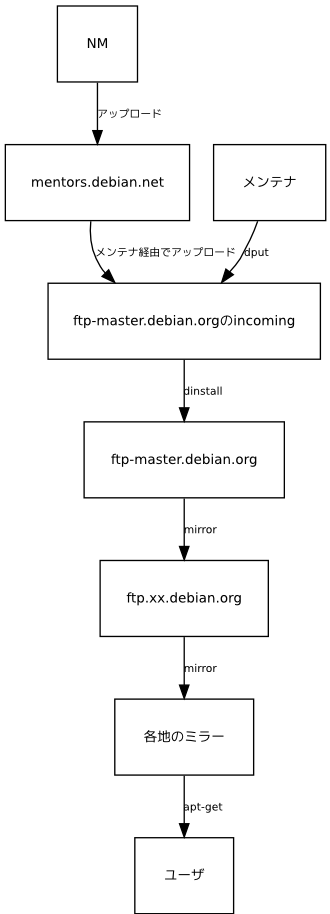
\includegraphics[height=0.8\vsize]{image200801/maint-package.png}

 \subsection{開発者のパッケージングの契機}

開発者がパッケージを作成するタイミングとはどういうものがあるでしょうか。
簡単にいうと三つあります:

 \begin{itemize}
 \item Debianに存在しない全く新しいパッケージ(ITPからの一連の流れをふむ)
 \item Debianにすでに存在しているパッケージの新しいアップストリームバージョンがリリースされた
 \item Debianにすでに存在しているパッケージにユーザがバグ報告をし、
       BTSに登録されたバグ報告の内容に対応するにはパッケージの修正が必要
       になった
  \item 依存関係が更新されたから更新
 \end{itemize}

\begin{figure}[h]
%inkscape --export-text-to-path --export-eps=devel-logic-i.eps devel-logic-i.svg 
 \begin{center}
  \includegraphics[width=0.8\hsize]{image200801/devel-logic-i.eps}
 \end{center} 
 \caption{開発者のロジックの流れ}
\end{figure}

 \subsection{作業の流れ}
 \subsubsection{アップストリームの取得}

新しいソースパッケージを取得します。tar.gz で公開されていればそのまま使
えます。tar.bz2 であったり、よくわからないアーカイブフォーマットだったり、
gitレポジトリでしか公開されていなかったりするので、それなりに加工します。

最初は適当に取得するわけですが、二回目移行はスクリプトで自動化して取得す
るようにします。watch という仕組みがあり、 uscan / uupdate コマンドで新しいバージョ
ンをダウンロードしてきてDebianパッケージ用のパッチを適用することができま
す。

\begin{figure}[h]
 \begin{commandline}
 version=3

 http://ftp.imendio.com/pub/imendio/giggle/src/giggle-(.*)\.tar\.gz

 \end{commandline}
\label{watchfile}
\caption{giggle パッケージの debian/watch ファイル}
\end{figure}


\subsubsection{パッケージング}

二度めからは差分の適用などで対応できるのですが、最初の新規パッケージの場
合はITPなどの処理を必要とします。また、新規にパッケージを作成するので、
なんらかのテンプレートパッケージから debian/ ディレクトリを取得してきて
修正するか、 dh\_make コマンドを利用してテンプレートを作成します。

この段階で debhelper を利用するのか、 cdbs を利用するのかの選択を迫られ
ます。cdbs は debhelper より新しい仕組みですが、2003年の登場から5年もたっ
ているのでそろそろこなれています。簡単なパッケージであれば cdbs を利用す
ればよいでしょう。現状の cdbs のフレームワークで不具合があるような場合で
あれば debhelper で詳細に設定するのがよいでしょう。

\begin{commandline}
$ dh_make 

Type of package: single binary, multiple binary, library, kernel module or cdbs?
 [s/m/l/k/b] b

Maintainer name : Junichi Uekawa
Email-Address   : dancer@debian.org 
Date            : Fri, 18 Jan 2008 22:22:51 +0900
Package Name    : tttt
Version         : 2.2
License         : blank
Type of Package : cdbs
Hit <enter> to confirm: 
Could not find tttt_2.2.orig.tar.gz
Either specify an alternate file to use with -f,
or add --createorig to create one.
[22:22:55]coreduo:tttt-2.2> 
\end{commandline}

 \subsubsection{BTSとの対応}

BTSに登録されているバグ報告に対してメールで対応したりします。
報告されている不具合をちゃんと修正してみたりします。

BTSは閲覧はWebでできますが、制御はWebではできません。BTSはメールで命令を
直接うって制御できます。メールコマンドはすぐに忘れてしまうので、
\texttt{/usr/share/doc/debian/bug-*} あたりを参照しながら作業します。BTSの
操作に便利なツールがいくつかあるので、そちらを利用することをおすすめしま
す。

\begin{itemize}
 \item  reportbug-ng 
 \item  reportbug
 \item  dpkg-dev-el 
\end{itemize}

 \subsubsection{ChangeLog の管理}

パッケージの新しいバージョンを作成する場合には、debian/changelog に対応
内容を記述します。
ここで活用できるツールには次があります。

\begin{itemize}
 \item devscripts の dch
 \item dpkg-dev-el の debian-changelog.el
 \item vim の debchangelog 
\end{itemize}

バージョン番号を自動で増加させてくれたり、いろいろなエントリーの補完など
をしてくれます。BTSを参照して修正されたバグのタイトルから ChangeLog のエ
ントリを生成してくれたりもします。

\begin{commandline}
pbuilder (0.177) unstable; urgency=low

  [ Loic Minier ]
  * Run apt-get autoremove after upgrade.

  [ Junichi Uekawa ]
  * python-apt/gdebi based pbuilder-satisfydepends-gdebi (closes:
    #453388)
  * Fix devpts mount permissions (closes: #453862)
  * Document pbuilder-satisfydepends-gebi in manpage

 -- Junichi Uekawa <dancer@debian.org>  Wed, 26 Dec 2007 20:53:24 +0900

\end{commandline}

\subsubsection{ビルド・テスト}

debian/以下のファイルを微調整して、パッケージをビルドします。
dpkg-buildpackage を直接呼び出してもよいですが、devscripts パッケージの
debuildコマンドを利用すればよいでしょう。

lintian / linda で生成されたパッケージにあきらかな間違いがないことを確認
します。

debc, debdiff で生成されたパッケージにあきらかな間違いや意図しない大きな
変化がないことを確認します。

debi でパッケージをインストールして正常に動作することを確認します。

pbuilder でビルドしてみて問題ないことを確認します。

pbuilder のテストスクリプトpbuilder-test を利用してインストール・アンイ
ンストール・アップグレードの試験をしてみるとさらによいでしょう。

 \subsubsection{アップロード}

署名してアップロードします。dpkg-buildpackage コマンドを利用してパッケー
ジをビルドすると自動でgpgで署名することになります。あとで署名しなおす場
合には、 debsign を利用します。

アップロードは dput コマンドを利用します。

 \subsection{非公式パッケージレポジトリの作成方法}

 テスト用に非公式のパッケージレポジトリを準備すると便利です。

 Packages.gz ファイルなどを生成してHTTP経由でアクセスできるようにしておく
 と、ユーザが /etc/apt/sources.list に追記することで apt を利用してパッケー
 ジが取得できるようになります。

 \begin{itemize}
  \item dpkg-scanpackages / dpkg-scansources を直接利用する方法。
  \item apt-ftparchive を利用する方法。
  \item mini-dinstall を利用する方法。
  \item apt-move を利用する方法。
  \item debarchiver
  \item reprepro
  \item dak
 \end{itemize}

2007年9月号で apt-ftparchive が紹介されていたので再掲します。

\subsubsection{apt-ftparchive}
 Sources.gz / Packages.gz などのパッケージ情報用ファイルを作成するためのツール。
 自分で作ったパッケージを apt-line として公開したいときに使います。
\begin{commandline}
  % apt-ftparchive packages . | gzip -9 > Packages.gz 
  % apt-ftparchive sources . | gzip -9 > Sources.gz
  % apt-ftparchive release . > Release 
\end{commandline}

\subsubsection{apt-sortpkgs}
 Packages ファイル および Sources ファイルをソートします。apt-ftparchive で作成したものはソート
 されていなかったりするので、アルファベット順にソートするときに使います。
\begin{commandline}
 % apt-sortpkgs Packages > Packages.sort
\end{commandline} 

 \subsection{参考文献}

 必読の文献として、以下があります。一通り読んだ後は、パッケージとしてイン
 ストールしておき、手元で検索できるようにしておくと便利です。sidを利用
 しているのであれば、パッケージとしてインストールしておくと最新版に勝手に
 更新されるため、便利です。内容に誤記などがあれば、ぜひBTSにバグ報告を登録してください。

 \begin{itemize}
 \item debian-policy: Debian Policy Manual。
       パッケージの準拠すべきルールが文書化されています。
 \item developers-reference: Developers Reference。
       
 \item doc-debian: Debian Project Documentation。 BTSのメールインタフェー
       スなどの文書がある。
 \item maint-guide: Debian New Maintainer's guide。
       New Maintainerとして知るべきマナーのようなものが文書化されています。
 \end{itemize}


%\end{multicols}

%===========================================================%
\dancersection{Debianパッケージにおいてのライセンスの取扱い}{上川 純一}
%===========================================================%
\label{sec:license}
\index{license} 
\index{copyright}
\index{ちょさくけん@著作権}
\index{らいせんす@ライセンス}

Debian Project の作成するディストリビューション Debian GNU/Linux はフリー
ソフトウェアから構成されています。Debian Projectにおいての「フリー」の定
義は DFSG というガイドラインで定められています。
それでは、それが実際にどういう使い方をされているのかを紹介します。

\subsection{なぜDFSGが必要なのか}

フリーソフトウェアにもいくつかの考え方がありえます。どれが正しいというわ
けではないので、一つに統一することはできないでしょう。具体的には次の三種
類くらいを考えればよいでしょう。

\begin{itemize}
 \item 自由なものを自由でありつづけさせたいライセンス(GPLなど)
 \item 自由なものを不自由にする自由も与えたいライセンス(MIT, BSDなど)
 \item 自分の作ったものは自由につかってくれてよいが、自分の作成したもの
       は完全なため、勝手にいじってほしくない。よって、変更したものについて
       は明示的にしておいてほしいもの(LPPL 1.0など)
\end{itemize}

複雑な例を挙げると、昔の\LaTeX{}関連のライセンス LPPL 1.0 では、変更した
ものについてはファイル名を変更することを義務としていました。また、現在で
もgnuplot ではオリジナルのソースコードの配布を義務とし、オリジナルのソー
スコードとパッチという形での配布のみ認めています。

もともとの開発者と開発に携わろうとしている人たちにとっては大きな違いがあ
りますが、エンドユーザにとってはフリーソフトウェアとして、利用できること
に関してはあまり大きな違いはありません。

Debian はそのどちらの立場でもなく、ディストリビュータとして関わることに
なります。許諾された範囲で次のことができればよいことになります:

\begin{itemize}
 \item Debian を有償・無償を問わず配布すること(DVD・公開ミラー・非公開
       ミラー)
 \item Debian を改変すること(Debianの改良、Debian外への流用、Debianから
       の派生ディストリビューションの開発など)
 \item Debianをあらゆる用途で利用できること(商用・教育用・宗教用・軍事
       用・医療用などを問わない)
\end{itemize}

これらを現実的に阻害しないようなライセンスの条件を取りまとめたのがDFSGです。

\subsection{DFSG全文}

DFSG全文を\fgref{fig:dfsg}に掲載します。

\begin{figure}[h]
 \begin{multicols}{2}
 {\small
     1. Free Redistribution

       The license of a Debian component may not restrict any party from
       selling or giving away the software as a component of an aggregate
       software distribution containing programs from several different
       sources. The license may not require a royalty or other fee for
       such sale.

    2. Source Code

       The program must include source code, and must allow distribution
       in source code as well as compiled form.

    3. Derived Works

       The license must allow modifications and derived works, and must
       allow them to be distributed under the same terms as the license
       of the original software.

    4. Integrity of The Author's Source Code

       The license may restrict source-code from being distributed in
       modified form {\bf only} if the license allows the distribution of
       "patch files" with the source code for the purpose of modifying
       the program at build time. The license must explicitly permit
       distribution of software built from modified source code. The
       license may require derived works to carry a different name or
       version number from the original software. (This is a compromise.
       The Debian group encourages all authors not to restrict any files,
       source or binary, from being modified.)

    5. No Discrimination Against Persons or Groups

       The license must not discriminate against any person or group of
       persons.

    6. No Discrimination Against Fields of Endeavor

       The license must not restrict anyone from making use of the
       program in a specific field of endeavor. For example, it may not
       restrict the program from being used in a business, or from being
       used for genetic research.

    7. Distribution of License

       The rights attached to the program must apply to all to whom the
       program is redistributed without the need for execution of an
       additional license by those parties.

    8. License Must Not Be Specific to Debian

       The rights attached to the program must not depend on the
       program's being part of a Debian system. If the program is
       extracted from Debian and used or distributed without Debian but
       otherwise within the terms of the program's license, all parties
       to whom the program is redistributed should have the same rights
       as those that are granted in conjunction with the Debian system.

    9. License Must Not Contaminate Other Software

       The license must not place restrictions on other software that is
       distributed along with the licensed software. For example, the
       license must not insist that all other programs distributed on the
       same medium must be free software.

   10. Example Licenses

       The "GPL", "BSD", and "Artistic" licenses are examples of licenses
       that we consider "free".
 }
 \end{multicols}
\caption{The Debian Free Software Guidelines (DFSG)}
\label{fig:dfsg}
\end{figure}


\subsection{ライセンス管理にかかわるプロセス}

Debian GNU/Linux で、ライセンス管理に関連するプロセスや仕組みを整理しま
しょう。

\subsubsection{ITP}

Debian ディストリビューションにパッケージを追加するのなら、最初に「ITP」
を行います。まずここでライセンスも付記することになり、特殊なライセンスで
あったら、議論になります。

\subsubsection{debian-legal}

複雑な条件や新規の状況が発生した場合には、debian-legal メーリングリストで
議論します。メーリングリストでコンセンサスが醸成されたり、されなかったり
します。フレームウォーが展開されたりします。結論はなかなか出ませんが、い
ろいろな視点が展開されるので見ているとおもしろいです。

\subsubsection{NEW キュー}

ITP後パッケージをアップロードすると、メーリングリストの議論とはあまり関係
ない方向で、ftp-masterがdebian/copyright を確認し、パッケージを承認し、
新しいパッケージがディストリビューションに入ります。この時点でDebianとし
てこのパッケージをこのライセンスで配布することはDFSG フリーであるという判
断をしたことになります。

この判断をくつがえすには、パッケージに対して、ライセンスが間違っていると
serious バグを報告することになります。

\subsubsection{再配布}

ftp-master に一旦入ると、Debian をミラーしている各サーバで再配布されるこ
とになります。また、CDROMイメージなどでも再配布されることになります。

各国の著作権法では著作物の複製は基本的には許諾がなければ許可されないとい
うルールです。そのため、Debian としてはライセンスの条件に同意して複製して
いるという考え方をとっています。各ミラーが到底許諾できないような条項は受
け入れられません。

\subsubsection{改変}

ユーザはダウンロードしたDebianの一部を改変します。
ユーザは改変をする際には、各パッケージの許諾にしたがっています。

\subsection{パッケージ作成においての debian/copyright 作成の実際}

Debian パッケージを作成する際に、ライセンス関連を確認します。
著作権は原則として許諾がないと「利用」ができないという類の権利です。
Debianパッケージの場合、その情報をdebian/copyrightファイルに整理します。

では、ライセンスはどうやって確認するのでしょうか。原作者はフリーソフトウェ
アとして一旦公開することを決心したのですから、良心的にライセンス情報をあ
る程度整理してくれているはずです。しかしながらその内容は監査の手続きが確
立されているわけでもなく、標準が存在するわけでもないので一律ではありませ
ん。また、よくあることですが、本人以外でその点を注意して確認しようとした
のは今Debian パッケージ作業をしようとしているあなたが初めてかもしれません。
必要事項が記述されていないこともありうるため、その場合は原作者に確認をと
りましょう。

ライセンス関連の情報は、通常はマニュアルやウェブページに記述されています。
そこで大まかな状況を確認します。例えば、failmallocパッケージを例にとって
みてみましょう。failmalloc のソースディレクトリを見てみます。

\begin{commandline}
$ ls
AUTHORS  ChangeLog  Makefile.am  NEWS	 THANKS      configure	   debian   failmalloc.c  ltmain.sh  mkinstalldirs
COPYING  INSTALL    Makefile.in  README  aclocal.m4  configure.ac  depcomp  install-sh	  missing
\end{commandline}

まずCOPYINGファイルがあるのがわかります。これはFSFの出しているライセンス
に多く、GPL全文が入っている場合が多いです。この場合は内容を確認してみると、
LGPL v2.1 の全文が入っていました。

\begin{commandline}
                  GNU LESSER GENERAL PUBLIC LICENSE
                       Version 2.1, February 1999

 Copyright (C) 1991, 1999 Free Software Foundation, Inc.
 51 Franklin Street, Fifth Floor, Boston, MA  02110-1301  USA
 Everyone is permitted to copy and distribute verbatim copies
 of this license document, but changing it is not allowed.

[略]
\end{commandline}

他にも、マニュアルなどにライセンスについて記述されている事が多いです。確
認してみましょう。今回は README, AUTHORS, ChangeLog, THANKS を確認しても
特にライセンス関連の記述はありませんでした。

あと、最終的にソースコードそれぞれのライセンスを確認しましょう。別のプロ
ジェクトからコピーしてきたファイルなどが含まれることもあり、別のライセン
スのものが混じっている可能性もあります。failmalloc.cを確認すると、ライセ
ンスについて明言している文面があるのが分かり、COPYINGファイルと整合性がと
れているのが確認できます。

\begin{commandline}
/* failmalloc - force to fail in allocating memory sometimes */
/*
 * Copyright (C) 2006 Yoshinori K. Okuji <okuji@enbug.org>
 *
 * This library is free software; you can redistribute it and/or
 * modify it under the terms of the GNU Lesser General Public
 * License as published by the Free Software Foundation; either
 * version 2.1 of the License, or (at your option) any later version.

 * This library is distributed in the hope that it will be useful,
 * but WITHOUT ANY WARRANTY; without even the implied warranty of
 * MERCHANTABILITY or FITNESS FOR A PARTICULAR PURPOSE.  See the GNU
 * Lesser General Public License for more details.

 * You should have received a copy of the GNU Lesser General Public
 * License along with this library; if not, write to the Free Software
 * Foundation, Inc., 51 Franklin Street, Fifth Floor, Boston, MA  02110-1301  USA
*/
\end{commandline}

今回は特にありませんが、バイナリデータファイルなども確認しておくとよいで
しょう。mp3ファイルや、画像データなど、本当に作者に権利があるのか念のため
確認しておくとよいでしょう。例えば調べた結果音楽データが Creative
Commons ライセンスで許諾されているのであれば、それは別のライセンスのファ
イルであるとして debian/copyright に記述します。

また、インストールされるバイナリがソースコードから生成されていることを確
認します。\footnote{ROMから吸い出したバイナリファームウェアが入っている
「フリーソフト」もあるので注意しましょう。} ソースコードから全部のバイナ
リが作成できないのであれば、原作者に問い合わせるステップが必要になること
もあります。

そうやって調査した一連の内容を debian/copyright に整理して記述します。複数の許諾
者や許諾内容がある場合はそれがわかるように整理しましょう。
この場合は、LGPLである旨を記録し、あとDebianパッケージ関連のスクリプトに
ついても他の部分と同じライセンスであるLGPL2.1に従うということを明記
しています。

\begin{commandline}
 This package was debianized by Hideki Yamane (Debian-JP) <henrich@debian.or.jp> on
Sat, 26 Jan 2008 09:28:51 +0900.

It was downloaded from http://www.nongnu.org/failmalloc/

Upstream Author: 

    Yoshinori K. Okuji <okuji@enbug.org>

Copyright: 

    Copyright 2006 Yoshinori K. Okuji

License:

    This package is free software; you can redistribute it and/or
    modify it under the terms of the GNU Lesser General Public
    License as published by the Free Software Foundation; either
    version 2.1 of the License.

    This package is distributed in the hope that it will be useful,
    but WITHOUT ANY WARRANTY; without even the implied warranty of
    MERCHANTABILITY or FITNESS FOR A PARTICULAR PURPOSE.  See the GNU
    Lesser General Public License for more details.

    You should have received a copy of the GNU Lesser General Public
    License along with this package; if not, write to the Free Software
    Foundation, Inc., 51 Franklin St, Fifth Floor, Boston, MA  02110-1301 USA

On Debian systems, the complete text of the GNU Lesser General
Public License can be found in `/usr/share/common-licenses/LGPL-2.1'.

The Debian packaging is (C) 2008, Hideki Yamane (Debian-JP) <henrich@debian.or.jp> and
is licensed under the LGPL-2.1, see `/usr/share/common-licenses/LGPL-2.1'.


\end{commandline}

なお、\texttt{/usr/share/common-licenses} に一般的に使われるライセンス文
\footnote{現在は Artistic, BSD, GFDL, GPL, LGPL}が用意されており、一般的
な文面の場合はそれを引用することでよいことになっています。そうでない場合
はライセンス文を全文 debian/copyright ファイルの中に転記します。

メンテナがこうやって準備した debian/copyright ファイルは、Debian ユーザ
は \texttt{/usr/share/doc/パッケージ名/copyright} で確認できます。



%===========================================================%
\dancersection{Debianパッケージ作成:データだけのパッケージ}{David Smith}
%===========================================================%
\label{sec:datapackage}
\index{でーただけのぱっけーじ@データだけのパッケージ}
\index{ぱっけーじ@パッケージ}
\index{deb}

Debianパッケージ作成にようこそ!dpkgのパッケージ、いわゆるDebianパッケー
ジの作成を分かりやすく、実例の分析に基づいて説明します。\footnote{Debianパッ
ケージが作りたいですよね。一応作りたいと前提に思っているからよろしくお願いします。}今回
データーだけのパッケージについてみてみましょう。

データーだけのパッケージは何かと言えばフォントやドキュメンテーションや
設定ファイルなどのパッケージを指します。要するにプログラムとライブラリではな
いパッケージではないということです。今回、GNOMEデスクトップの壁紙ファイルを集めたもの、
gnome-backgroundsの構成を元に説明します。Debian Popularity
Contest\footnote{Debian Popularity Contest の
URL:\url{http://popcon.debian.org/}}によると現在 gnome-backgrounds が殆ど
全部のGNOMEインストールに含まれていて、GNOMEを使用していれば
gnome-backgroundsも入っているはずです。背景ファイルですが、パッケージの構成に複
雑な部分もあると思いますので、細かいところまで見てみようと思います。

\subsection{準備}

まず、Debian New Maintainer's Guide
\footnote{Debian New Maintainer's Guide の URL:
\url{http://www.debian.org/doc/devel-manuals\#maint-guide}}
のページを開いておいたらいいでしょう。不明な点があった場合、
New Maintainer's Guideに分かりやすく書いていますし、質問があった場合は何処まで送れば良いか
書いてあります。

次に gnome-backgrounds のソースパッケージをダウンロードしましょう。
\begin{commandline}
$ apt-get source gnome-backgrounds
\end{commandline}
% $ - hi emacs

準備の最後にパッケージの構成に必要な依存パッケージをインストールしなけれ
ばビルドが出来ないので以下のコマンドをインストールしましょう。
\begin{commandline}
$ apt-get build-dep gnome-backgrounds
\end{commandline}
% $ - hi emacs

\subsection{基本のDebianパッケージファイル}

今のところ、apt-get sourceがソースパッケージをgnome-backgrounds-2.20.0と
いうディレクトリに展開されています。そのディレクトリの中にはdebian/ディレクトリが
あり、そこにパッケージ作成の設定ファイルがあります。パッケージによるファイル
数が異なるが、gnome-backgroundsは必要最低限のもので構成されています。

\begin{commandline}
piyo:/tmp/gnome-backgrounds-2.20.0> ls -l debian/
合計 36
-rw-r--r-- 1 dds dds 3755 2008-03-08 16:21 changelog
-rw-r--r-- 1 dds dds    2 2008-03-08 16:21 compat
-rw-r--r-- 1 dds dds 1022 2008-03-10 15:11 control
-rw-r--r-- 1 dds dds  771 2008-03-08 16:21 control.in
-rw-r--r-- 1 dds dds 1780 2008-03-08 16:21 copyright
-rwxr-xr-x 1 dds dds  368 2008-03-08 16:21 rules
-rw-r--r-- 1 dds dds  145 2008-03-08 16:21 watch
\end{commandline}

この中でchangelog、control、copyright、rulesはあらゆるパッケージに
必要なファイルです。

\subsubsection{debian/copyright}

\texttt{debian/copyright}は上流ソースコード、データーなどの著作権を認めるためのファ
イルです。形式は自由ですが、パッケージビルドツールに対して必須なので自分専用でも自
分の会社内専用のパッケージでも一応書く必要があります。最低限として
「All Rights Reserved」と書いてもよいです。gnome-backgroundsの
\texttt{debian/copyright}ファイルが長すぎるのでここには示しませんが、気になる
方は見てみてください。
このファイルはパッケージをインストールすると\texttt{/usr/share/doc/パッケージ名/copyright}
にインストールされます。

\subsubsection{debian/changelog}

\texttt{debian/changelog}にはパッケージのバージョンを記録します。必ずしもパッケージの
バージョンが上流のバージョンに一致することではないので必須になっています。それにパッ
ケージの最新バージョン番号はこのファイルの最初の1行目から直接に抽出されます。

gnome-backgroundsの最新バージョンのchangelogを見てみましょう。
\begin{commandline}
gnome-backgrounds (2.20.0-1) unstable; urgency=low

  * New upstream release.

 -- Sebastian Dr\"oge <slomo@debian.org>  Sat, 22 Sep 2007 09:49:38 +0200
\end{commandline}

かなりシンプルです。しかし、空白と日付の形式を厳守しなければビルドするときにエラー
が発生するから注意しましょう。\footnote{debchange(1)というツールで手軽にchangelog
編集が出来ます。devscriptsというパッケージで提供されています。}

\subsubsection{debian/control}

\texttt{debian/control}にはパッケージ名、Maintainer、依存のパッケージなどのメタ情
報が記されています。gnome-backgroundsの場合、独特として\texttt{debian/control}と共に
\texttt{debian/control.in}ファイルもあります。\texttt{debian/control.in}はDebianのパッケージツー
ルに対して関係ないから無視しても良いです。
Gnomeプロジェクトは規模が大きいのでメンテに関わっている人が多いです。
\texttt{debian/control}にアップロード出来る人達の名前が記載されていますが、
人の名前が多すぎて直接管理しにくいので、@GNOME\_TEAM@という変数だけを書いています。
そして別のファイルにその人達の名前を書いて、発行時にスクリプトによって変
数を置換します。

では\texttt{debian/control}を見てみましょう。
\begin{commandline}
Source: gnome-backgrounds
Section: gnome
Priority: optional
Maintainer: Sebastien Bacher <seb128@debian.org>
Uploaders: @GNOME_TEAM@
Build-Depends: debhelper (>= 5), cdbs, gnome-pkg-tools
Build-Depends-Indep: libxml-parser-perl
Standards-Version: 3.7.2

Package: gnome-backgrounds
Architecture: all
Depends: ${misc:Depends}
Description: a set of backgrounds packaged with the GNOME desktop
 This is a collection of desktop backgrounds created with GNOME users in mind.
 It contains the following backgrounds:
 .
[後略]
\end{commandline}

第一段落にソースパッケージを記述します。apt-get sourceとapt-get buildd-dep
を実行する時、ソースパッケージの情報を使っています。9行目以降に作成する
gnome-backgroundのバイナリパッケージを定義しています。順番に関してはソース
パッケージが必ず最初に記述されます。そしてSource又はPackageはそれぞれの段落の最初の
1行に書きます。それ以外の中身の項目は特に決まった順番がありません。

SectionとPriorityとの項目は少しややこしいです。決まった選択肢の中
から1つしか選べないので合わない場合があるけどgnome-backgroundsの場合はぴっ
たり、gnomeでoptional。選択肢の詳しい情報はDebian Policy Manualに書いてあ
ります。\footnote{Debian Policy Manual
URL:\url{http://www.debian.org/doc/debian-policy/ch-archive.html\#s-subsections}}
後はMaintainerとUploadersはそれぞれ書いた通りです。Uploadersは共同にメンテを
している人になります。つまり、Maintainerの項目は必ず一人しか書けないけど他の
人もメンテしていればUploadersに書くということになります。

次にビルドのための依存関係パッケージが書いてあります。殆どのパッケージにはビ
ルドするための依存パッケージと、利用するための依存パッケージが異なります。例え
ば普通のプログラムの場合にC/C++のヘッダーがビルド時に必要ですが、実行する時には
必要ないパッケージがあり、これらを分けて書いています。
\footnote{Build-DependsとBuild-Depends-Indepの違いがあまり分からなくてす
みません!}gnome-backgroundsがビルド時に使ってる依存パッケージがより典型
的なのでそれぞれ少し説明します。

\begin{description}
 \item[cdbs]
            {\bf Common Debian Build System} の省略, 共有されているビルドシステムです。
            多くの人が使っていると思います。
 \item[debhelper]
            いろいろパッケージビルドに役に立つツールです。例えば上流のドキュメンテー
            ションを自動的にインストールするツールなどが提供されています。
 \item[gnome-pkg-tools]
            cdbsに少し似ている感じでGNOMEパッケージを作るのに役に立つツー
            ル群です。
 \item[libxml-parser-perl]
            PerlのXML::Parserモジュールを提供するパッケージです。
\end{description}

ソースパッケージの段落の最後にStandards-Versionという項目はDebian
Policy Manualの何バージョンに準拠しているかを説明します。

続いてバイナリパッケージの項目になります。パッケージ名が最初に来ます。それから
対応するアーキテクチャーを書きます。データーだけのパッケージの場合にもall
にしても良いです。今度のバイナリパッケージ作成発表にallの他を説明します。その他
はDependsラインにruntimeの依存関係のパッケージ(この場合は自動的に抽出さ
れる)が書いていて、最後にパッケージの説明を記述します。
詳しくはDebian Policy Manualを参照してください。

\subsubsection{debian/rules}

\texttt{debian/rules}でパッケージのビルドがどう行われるかを定義します。中身の形式は
完全自由ですが、外部のツールがPolicy Manualに書いている呼び出し方に依存してい
ます。それでMakefile形式を用いているパッケージの割合は100\%に近いです。
しかしMakefileなのにcdbsを使っているので普通のMakefileにほとんど似ていません。
時間と労力を節約したい方は cdbs を是非試してください。

gnome-backgroundsの\texttt{debian/rules}を見てみましょう。

\begin{commandline}
#!/usr/bin/make -f

include /usr/share/cdbs/1/rules/debhelper.mk
include /usr/share/cdbs/1/class/gnome.mk
include /usr/share/cdbs/1/rules/simple-patchsys.mk
include /usr/share/gnome-pkg-tools/1/rules/uploaders.mk
-include /usr/share/gnome-pkg-tools/1/rules/gnome-get-source.mk

binary-post-install/gnome-backgrounds::
	rm -rf debian/gnome-backgrounds/usr/share/locale
\end{commandline}
% )$ -- hello emacs

殆ど以前に定義しているルールを再利用しているだけです。1つだけのこのパッ
ケージに特別に追加している箇所があります。
それはbinary-post-install/gnome-backgrounds::の
ところです。gnome-backgroundsというバイナリパッケージを作ってから、
必要ないのでそのディレクトリを削除する、という意味です。

\subsubsection{debian/watch}

\texttt{debian/watch}ファイルは不要ですが、自動的に新しい上流のソフトを取得し
てビルドする仕組みを利用する場合に使用します。

\subsection{パッケージビルド}

上記を設定してから、パッケージのビルド自体はdpkg-buildpackage又は
debuildコマンドだけで出来きます。設定以来の変更を\texttt{debian/changelog}ファイルに
記録するとバージョン管理ができます。dpkg-buildpackageの出力が長いので、ここでは説明
しませんが、各自で確認してみてください。

\dancersection{バイナリ一つだけのパッケージを作成してみる}{吉田 俊輔}
\label{sec:binpkg}
\index{ばいなりひとつだけのぱっけーじ@バイナリ一つだけのパッケージ}
\index{ぱっけーじ@パッケージ}
\index{deb}

\subsection{前提/対象者}

この記事はDebianパッケージを作った経験が無い人むけに一番わかりやすいと思われる
dh\_makeを使ったパッケージの作成について説明しています。

前提知識としてはある程度make(Makefile)を理解している必要がありますが、
多くはありません。若干はこのドキュメント中で説明します。

\subsection{debパッケージを作る/使う理由・メリット}

通常のパッケージシステムのメリットとしてtarボール(*.tar.gzなどで圧縮されたアーカイブファイル)を
使った場合に比較して、複数マシンへのインストール、環境再現が簡単、便利、
パッケージのアンインストール、バージョンアップが容易といった点が挙げられ
ます。

debパッケージを作るメリットとしては、それらに加え、
ソースファイルとパッチファイルの管理が簡単、ビルドに必要な環境(のパッケージ)を整備するのが
簡単、等のメリットが挙げられるでしょう。

もちろんパッケージを作りたい理由は人それぞれと思いますが、
自分の使いたいアプリ/機能がパッケージになっていないという理由が多いでしょ
う。

Debian開発者になるためと言う人もいるかもしれません。


\subsection{dh\_makeとは}
dh\_makeコマンドはdh-makeパッケージに含まれるコマンドで、
パッケージを作る際に一般的な内容のひな形を
作ってくれるツールです。

ソフトウェアのソースコードを展開したディレクトリの中で、
このコマンドを実行すると、対話的なやりとりを行ったあと、
ひな形としてdebhelperスタイルのディレクトリとファイルを準備します\footnote{CDBSスタイルのひな形も作成可能です。}。

\subsection{debhelperスタイル}
debパッケージを作る方法(スタイル)についてはいくつかあります。
今回説明するのはdh\_makeのdebhelperスタイルについてです。
そのほかに同様にdebhelperスタイルを使用したdpatch,CDBS,dbs,quilt,yadaと
いったスタイルがあるそうです。

その他にもスクリプト言語向け等にもいくつかスタイルがあるようです。
debhelperスタイルはdebianではもっとも一般的でシンプルなスタイルです。
現在のdebianパッケージで採用しているパッケージの割合がもっとも多いと言われています。
基本的にdh\_コマンドをrulesというファイルからから呼び出す形式となります。

\subsection{dh\_makeでのdebhelperスタイルのパッケージ作成に最低限必要なファイル}

dh\_makeが作成する、debhelperスタイルのパッケージ作成に
最低限必要なファイルとして以下の2つのディレクトリと、
4つのファイルがあります。

まず、作業に使うディレクトリ名の形式が決まっています。
その下にdebianディレクトリが作成され、パッケージングに必要なファイルはここにすべて置かれます。
必要なファイルについてはひな形がdh\_makeで準備されます。
\begin{commandline}
softname-version/ (ディレクトリ名)
  debian/ (Debianディレクトリの存在=debパッケージが作成可能)
     control (パッケージ情報:パッケージ名、バージョンの記述)
     changelog (更新履歴)
     copyright (著作権情報の記述)
     rules (rulesパッケージの作成方法を記述)
\end{commandline}

\subsection{その他のファイル}

以下はdh\_makeが準備するサンプルのファイルです。
これらも同様にdh\_makeでdebianディレクトリの下に準備されます。
必須ではありませんので、必要に応じて利用します。

\begin{commandline}
debian/
  README.Debian(オリジナルとパッケージ化したときの差分情報)
  conffiles.ex(設定ファイル名のリスト)
  cron.d.ex(cronで実行するファイル名リスト)
  dirs
  docs
  init.d.ex(サービスの起動スクリプト)
  manpage.1.ex, manpage.sgml.ex(manファイル)
  preinst.ex(インストール前のスクリプト)
  postinst.ex(インストール後のスクリプト)
  prerm.ex(アンインストール前のスクリプト)
  postrm.ex(アンインストール後のスクリプト)
  等
\end{commandline}

\subsection{新規作成の流れ}

db\_makeを使ったパッケージの新規作成の流れとしては以下のようになります。
\begin{itemize}
 \item 
 ソースアーカイブ展開
 \item  テンプレート作成
\begin{commandline}
 $ dh_make
       \end{commandline}
 \item  debianディレクトリ配下の編集
 \item changelog記述
 \begin{commandline}
 $ dch
       \end{commandline}
 \item 
 controlファイル(パッケージ名や依存関係を記述)
 \item 
 copyrightファイル(著作権情報の記述)
 \item 
 rulesファイル(ビルド手順の修正、確認、不要なコードの削除)
 \item 
       ビルド
 \begin{commandline}
 $ dpkg-buildpackage(debパッケージの作成)
 \end{commandline}
\end{itemize}

\subsection{ソースアーカイブ展開}

通常、tarボール等で配布されているファイルを展開し、
その展開されたディレクトリ名を修正(リネーム)します。

dh\_makeでひな形を作るためには packagename-version の
形式である必要がありますので、上記の形式になっていない場合は
適切にリネームを行ってください。

\subsection{dh\_make(debianディレクトリ、テンプレートの作成)}

dh\_makeでのひな形の作成です。

上記で適切な形式にリネームされたディレクトリにcdし、dh\_makeを
実行します。その際、可能ならライセンスの指定を行った方が良いでしょう。
後々の手間が省けます。

また、環境変数からメンテナ名とそのメールアドレスを取得しますので、
あらかじめ下記の環境変数を設定しておくことをおすすめします。
これも後々の手間が省けます。

dh\_makeを実行すると、パッケージの種類を選択します。
今回の例ではSingle binary (s)を選択します。

その他、許諾条件(ライセンス)の指定(-c)も可能です。
指定できる許諾条件(ライセンス)は gpl、lgpl、artistic、bsd です。

指定できるパッケージ種類は
Single binary (s)/Multiple binary (m)/Library (l)/Kernel module (k)/cdbs
(b) です。

環境変数は、DEBFULLNAME(メンテナ名)、DEBEMAIL(メールアドレス)で指定しま
す。

\subsection{dch(debian/changelogの記述)}

次に、debian/changelogの記述の記述について説明します。
まず、このファイルはテキストファイルですが、形式が厳密に決まっており、
直接エディタで修正するのはおすすめしません。

たとえば、
\begin{commandline}
$ dch -i 
\end{commandline}
を使えば定型の形式部分は自動的に記入できるのでおすすめです。

次に、debian/changelogの先頭にあるバージョン情報がこれから作成されるパッケージのバージョンとして
使用されます。必要なら修正を行ってください。

次がパッケージの状態ですが、通常はunstableで問題ありません。

次は緊急度ですがこれもlowで問題ないでしょう。

実際の変更履歴としての内容はアスタリスク(*)の後にコメントとして記述します。
その後の定型dchが作成してくれる内容をそのまま使うのが良いでしょう。

debian/changelog:
\begin{commandline}
 smp-mgzip (1.2c-1) unstable; urgency=low

  * Initial release (Closes: #nnnn)  <nnnn is the bug number of your ITP>

 -- yoshida syunsuke <koedoyoshida@gmail.com>  Sun, 30 Mar 2008 22:21:28 +0900
\end{commandline}


\subsection{controlの記述}
controlファイルにパッケージ名や依存関係を記述します。

ここではソースパッケージとバイナリパッケージで分けて記載します。

Sectionには main (完全にフリーなソフトウェア)、 non-free (実際の所フリー
であるとはいえないソフトウェア)、そして contrib (それ自身はフリーなソフ
トウェアであるけれども、non-free なソフトウェアが無ければ使えないもの)
があります。 更に、これらの下には各パッケージをおおまかに分類する論理的
なサブセクションが用意されており、 そこに含まれるパッケージの種類を簡単
に説明するような 名前がつけられています。 管理者専用のプログラムのために
「admin」、 基本的なツールのために「base」、 プログラマーのためのツール
が含まれる「devel」、 文書の「doc」、ライブラリの「libs」、 電子メールの
読み書きに使うリーダや 電子メールサーバを構築するためのデーモンは「mail」、
ネットワーク関係のアプリケーションやデーモンの「net」、 他のどんな分類に
もあてはまらないような X11 用の プログラムは「x11」など、そしてさらに多
くのものが 用意されています。デフォルトはmainですので、ここに記載すると
mainのサブセクションを指定するということになります。

Priorityはこのパッケージをインストールすることが ユーザにとってどれくら
い重要なものかを示しています。

新規パッケージの場合、優先度「optional」(選択可能) としておけば、通常
は問題無いでしょう。

バイナリパッケージについてはCPU等のアーキティクチャに依存する物(バイナリの実行ファイル等を含む場合)はany,スクリプトやドキュメントなどアーキティクチャに依存しない場合はallを指定します。
その他の項目は必要なら修正してください。

debian/control:
\begin{commandline}
Source: smp-mgzip(ソースパッケージ名)
Section: unknown(パッケージのセクション)
Priority: extra(パッケージの重要度)
Maintainer: yoshida syunsuke <koedoyoshida@gmail.com>(メンテナーの名前とメールアドレス)
Build-Depends: debhelper (>= 5), autotools-dev(ビルドに必要なパッケージ)
Standards-Version: 3.7.2(テンプレート作成に参照したDebianポリシー標準のバージョン)

Package: smp-mgzip(バイナリパッケージ名)
Architecture: any(対応アーキティクチャ)
Depends: ${shlibs:Depends}, ${misc:Depends}(パッケージの依存関係)
Description: <insert up to 60 chars description>(パッケージの説明)
 <insert long description, indented with spaces>
\end{commandline}

\subsection{copyrightの記述}

ファイルの著作権と許諾条件(ライセンス)についての記述です。

dh\_make実行時にライセンスを指定しておけばひな形が作成されます。
ソフトウェアによってはディレクトリやファイルごとに別のライセンスの場合も
ありますので、注意してください。

debian/copyright:
\begin{commandline}
 This package was debianized by yoshida syunsuke <koedoyoshida@gmail.com> on
 Sun, 30 Mar 2008 22:21:28 +0900.

 It was downloaded from <fill in http/ftp site>

 Upstream Author: <put author(s) name and email here>

 Copyright: <put the year(s) of the copyright, and the names of the
            copyright holder(s) here>

 License:
 (中略)
 On Debian systems, the complete text of the GNU General
 Public License can be found in `/usr/share/common-licenses/GPL'.

 The Debian packaging is (C) 2008, yoshida syunsuke <koedoyoshida@gmail.com> and
 is licensed under the GPL, see above.
\end{commandline}


\subsection{rulesの記述}
debian/rules
には
パッケージングを行うための手順を記述します。
Makefile形式の記述方法ですが、パッケージングの支援をするdh\_xxxコマンド
群(debhelperパッケージ)を並べるのがほとんどです。
dpkg-buildpackageが期待している必須ターゲットは:

\begin{commandline}
 build: (ビルド実行)
 binary: (バイナリパッケージの生成、通常binary-indepとbinary-archの実行)
 binary-indep: (アーキティクチャ独立のバイナリパッケージ作成)
 binary-arch:(アーキティクチャ依存のバイナリパッケージ作成)
\end{commandline}

\subsection{rulesの記述 buildターゲット}
dh\_makeのデフォルトの場合、buildターゲットはbuild-stampに依存している=
build-stampターゲット(make、コンパイル等の実作業)を呼び出します。

同様にbuild-stampはconfig.status(configureの実行)に依存しています。

\begin{commandline}
 
 debian/rules
 build: build-stamp

 build-stamp:  config.status
        dh_testdir

        # Add here commands to compile the package.
        $(MAKE)
        #docbook-to-man debian/smp-mgzip.sgml > smp-mgzip.1

        touch $@
\end{commandline}

\subsection{rulesの記述 binaryターゲット}
\begin{commandline}
 binary: binary-indep binary-arch

 binary-indep: build install

 binary-arch: build install
        dh_testdir
        dh_testroot
        dh_installchangelogs ChangeLog
       (中略)
        dh_builddeb
\end{commandline}

\subsection{rulesの記述 installターゲット}
\begin{commandline}
 install: build
        dh_testdir
        dh_testroot
        dh_clean -k  --exclude ./mgzip.c.orig
        dh_installdirs

        # Add here commands to install the package into debian/smp-mgzip.
        $(MAKE) prefix=$(CURDIR)/debian/smp-mgzip/usr install
\end{commandline}

\subsection{オリジナルのmakeファイルの修正}
Single binary (s)の場合、
Debianのパッケージングツールは\verb!$(CURDIR)/debian/(パッケージ名)/!以下にあるファイルをまとめてパッケージにします。

「make install」実行で\verb!$(CURDIR)/debian/(パッケージ名)/!以下にインストール
するようにオリジナルのtarball等から展開された、Makefileを準備します。

元々のMakefileが提供されていればそれを修正すればよいでしょう。無ければMakefileを作成してください。
詳細なMakefileの作り方については書籍「make 改訂版」を参照してください。

\subsection{パッケージ作成}

簡易なパッケージ作成のテストとして下記のコマンドを実行するとパッケージ作成が行われます。
\begin{commandline}
$ dpkg-buildpackage  -us, -uc  -rfakeroot
\end{commandline}

上記のファイルが適切に作成されていれば、以下のファイルが作成されます。
\begin{commandline}
 xxx-y.y.y_zzzz.deb(バイナリパッケージ)
 ソースパッケージ
 xxx-y.y.y.dsc(ソース概要:controlより生成)
 xxx-y.y.y_zzzz.diff.gz(パッケージ化用の差分)
 xxx-y.y.y.orig.tar.gz(オリジナルソースファイル)
 xxx-y.y.y_zzzz.changes(パッケージ変更点: control+changelog)

凡例: 
	xxx:パッケージ名
	y-y-y:バージョン,
	zzzz: Debian アーキテクチャ(i386,amd64,all,等))
\end{commandline}

上記の例でdpkg-buildpackageに渡しているオプションの意味は以下の物です。
\begin{itemize}
 \item  -us, -uc(gpgサインをしない)
 \item  -rfakeroot(一般ユーザでの作成)
\end{itemize}


\subsection{dpkg-buildpackageとdebuildの違い}

dpkg-buildpackageとよく似たプログラムにdebuildがあります。
違いとしては以下の点があります。

\begin{itemize}
 \item  dpkg-buildpackage:

 メリット dh\_makeで作ったばかりの設定ファイルでもdebを作成可能

 デメリット 一般ユーザで使用するときは-rfakerootの指定が必要
 \item  debuild:

 メリット -rfakeroot指定が省略可能、ルールに従ったチェックの実行を行っ
	てくれる。

 デメリット 各種ルールに従って設定ファイルを書かないとエラーや警告となる
 作成されるパッケージに関しては両方とも同じ
\end{itemize}


\subsection{ファイルへの署名}

これまでの例で、dpkg-buildpackageやdebuildで指定した -us -usのオプションは
ファイルへの電子署名を省略するためのオプションです。
\begin{itemize}
 \item  -us, -uc
 Do not sign the source package or the .changes file, respectively.
\end{itemize}
パッケージを
自分のみで使用する場合はともかく、外部へ公開することも視野にいれるのであ
れば、電子署名を行うのが適切でしょう。

debianパッケージに署名するにはGnuPGで鍵を用意し、パッケージ作成時にdebuild、dpkg-buildpackageを使用するとデフォルトでパッケージに署名が行われます。


\subsection{補足:ファイルの公開方法}

パッケージ公開用のファイル(Packages.gz,Sources.gz)を作ります。
\begin{commandline}
 $ apt-ftparchive packages . | gzip -c9 > Packages.gz
 $ apt-ftparchive sources . | gzip -c9 > Sources.gz
\end{commandline}

apt-ftparchiveコマンドはapt-utils パッケージに入っています。

\subsubsection{ローカルで確認}

sources.list(aptline)に以下のような記述を追加しapt-get update;apt-get installでインストールできるかを確認します
\begin{commandline}
 deb file:/usr/src/ ./
\end{commandline}

\subsubsection{ネットワークで確認}

ローカルで確認できたディレクトリ構成のまま、そっくりhttpで公開します。sources.list(aptline)も同様に記述します。
\begin{commandline}
 deb-src http://XXX ./
\end{commandline}

\subsection{補足:debソースファイルの展開とリビルド}

*.dsc,*.orig.tar.gz,*.diff.gzを入手して
展開し、

\begin{commandline}
 $ dpkg-source -x XXX.dsc
 $ cd 作成されたディレクトリ
\end{commandline}
必要なら修正を実施して
リビルドします

\begin{commandline}
 $ debuild (またはdpkg-buildpackage)
\end{commandline}

\subsection{参考資料}
\begin{itemize}
 
 \item  入門Debianパッケージ(ISBN:4-7741-2768-X)
 \item  Debian 新メンテナガイド
	\footnote{\url{http://www.jp.debian.org/doc/manuals/maint-guide/}}
 \item Debian GNU/Linux スレッドテンプレ 自作パッケージを作りたい
       \footnote{\url{http://debian.fam.cx/index.php?AptGet\#n8109a54\\}}
 \item make 改訂版(ISBN:4-900900-60-5)
\end{itemize}


\dancersection{バイナリをわけたパッケージの扱い}{前田 耕平}
\label{sec:multibinpkg}
\index{ふくすうばいなりのぱっけーじ@複数バイナリのパッケージ} 
\index{ぱっけーじ@パッケージ}
\index{deb}

\subsection{はじめに}

今回はDebianパッケージを作成した経験がほぼ無い人を対象とし、先月
\footnote{2008年4月} の『バイナリ一つだけのパッケージを作成してみる』を
予習していることを前提とします。

一応、前回の内容もおさらいしながら、今回もdh\_makeを使って、debhelperス
タイルでの複数のバイナリに分けてパッケージを作る方法を説明しますので、前
回参加できなかったとしても、ある程度は問題ないかと思います。

\subsection{バイナリの分け方の考え方}
通常のパッケージは、一つのバイナリパッケージとして作成・配布されるケー
スが多いでしょう。ではどのようなケースにおいて、バイナリパッケージは複数
に分けられているのでしょうか。大きく分けると次の三パターンくらいになりそう
です。

\begin{itemize}
 \item
開発環境と実行環境

例)
      \begin{itemize}
       \item
	    JavaのSDKとJRE

      \end{itemize}
 \item
C/Sモデルのサーバ側プログラムとクライアント側プログラム

例)
      \begin{itemize}
       \item
	    bindとdnsutils
      \end{itemize}

 \item
プログラム本体とアドオンで追加可能なモジュール、ユーティリティ

例)
      \begin{itemize}
       \item
	    ApacheとApache moduleやApache Bench
      \end{itemize}
\end{itemize}

これらに共通して言えるのは、単一のソースツリーから複数に分けることにより、
導入するユーザの使い勝手が良くなる、ということだと言えると思います。

なお、複数のバイナリパッケージを作成するときも、ソースツリー及びソースパッ
ケージ自体は単一なので、複数のソースツリー・ソースパッケージから生成され
る事はありません。

\subsection{前回のおさらい}

前回は、dh\_makeを使って、debhelperスタイルで単一のバイナリパッケー
ジを作りました。今回は、まず簡単なCのプログラムとMakefileを用意して、それを
Debianパッケージにします。そこで単一のバイナリパッケージの場合と複数のバ
イナリパッケージに分ける場合との違いを見てみましょう。

\subsubsection{ソースコードとMakefileの用意}
 まず、下記のようなディレクトリ、ファイルを用意します。
 \begin{commandline}
hoge-1.0/
 hoge.c
 Makefile
 \end{commandline}
 ファイルはそれぞれ下記のようなコードを書きます。
 \begin{itemize}
  \item
       hoge.c
       \begin{commandline}
#include <stdio.h>
      
int main(void)
{
       printf(``hello\n'');
       return 0;
}
       \end{commandline}
  \item
       Makefile
       \begin{commandline}
CC=gcc
CFLAGS=-O
BINDIR=/usr/games
     
hoge: hoge.c
       $(CC) $(CFLAGS) -o hoge hoge.c
       
install:
       install -d ${DESTDIR}${BINDIR}
       install -m 755 hoge ${DESTDIR}${BINDIR}
       
clean:
       rm -f hoge
       \end{commandline}
 \end{itemize}

\subsubsection{dh\_makeでテンプレートの作成}
それでは、前回と同様にdh\_makeを使ってシングルパッケージを作ってみます。
まず、dh\_makeでテンプレートを作ります。

\begin{commandline}
$ cd hoge-1.0

$ dh_make --single -c gpl --createorig
Maintainer name : Kouhei Maeda
Email-Address   : mkouhei@gmail.com
Date            : Sat, 10 May 2008 15:36:29 +0900
Package Name    : hoge
Version         : 1.0
License         : gpl
Type of Package : Single
Hit <enter> to confirm: 
Done. Please edit the files in the debian/ subdirectory now. You should also
check that the hoge Makefiles install into $DESTDIR and not in / .
\end{commandline}

\subsubsection{debianディレクトリ以下のファイルの編集}

debianディレクトリ以下を編集します。
\begin{commandline}
$ cd debian

$ rm *ex *EX (<-不要なサンプルファイルを削除します。)
\end{commandline}

\begin{itemize}
 \item
      debian/control
      \begin{commandline}
Source: hoge
Section: games
Priority: extra
Maintainer: Kouhei Maeda <mkouhei@gmail.com>
Build-Depends: debhelper (>= 5)
Standards-Version: 3.7.2

Package: hoge
Architecture: any
Depends: ${shlibs:Depends}, ${misc:Depends}
Description: sample program
 Hello hoge program
      \end{commandline}
 \item
      debian/copyright
      \begin{commandline}
This package was debianized by Kouhei Maeda <mkouhei@gmail.com> on
Sat, 10 May 2008 15:36:29 +0900.

It was downloaded from <http://www.palmtb.net>

Upstream Author(s):

    <Kouhei Maeda mkouhei@gmail.com>

Copyright: 

    <Copyright (C) 2008 Kouhei Maeda>

License:
(以下、省略) 
      \end{commandline}

 \item
      debian/dirs\footnote{hogeのインストール先を指定します。}
      \begin{commandline}
usr/games
      \end{commandline}

 \item
      debian/changelog
      \begin{commandline}
$ dch
hoge (1.0-1) unstable: urgency=low

  * Initial release

 -- Kouhei Maeda <mkouhei@gmail.com>  Sat, 10 May 2008 15:47:41 +0900
      \end{commandline}
\end{itemize}

\subsubsection{パッケージ作成}
それでは、debuildコマンドでパッケージを作成してみます。
\begin{commandline}
$ debuild -us -uc
\end{commandline}

debファイルができているのを確認します。
\begin{commandline}
$ cd ../../
$ ls hoge_1.0*
hoge_1.0-1.diff.gz  hoge_1.0-1_i386.build    hoge_1.0-1_i386.deb
hoge_1.0-1.dsc      hoge_1.0-1_i386.changes  hoge_1.0.orig.tar.gz
\end{commandline}

上記のような簡単なものであれば、rulesファイルを修正しなくても、パッケー
ジを作れる事が分かります。ちゃんとやるには、lintianのエラーや警告を潰し、
pbuilderでのチェックやインストール、アンインストールのチェックをする必要
がありますが、ここでは省略します。

\subsection{複数のバイナリパッケージを作ってみる。}
それでは、今度は先ほどの簡単なコードを一部変更して、それぞれ別のパッケー
ジになるようにします。

\subsubsection{ソースコード、Makefileの用意}
下記のようなファイルを用意します。先ほどのhoge-1.0をコピーして修正すれば
よいでしょう。

\begin{commandline}
foo-1.0/
 foo.c
 bar.c
 Makefile
\end{commandline}
各ファイルは下記のようにします。
\begin{itemize}
 \item
      foo.c
      \begin{commandline}
#include <stdio.h>

int main(void)
{
  printf(``hello,foo\n'');
  return 0;
}
      \end{commandline}
 \item
      bar.c
      \begin{commandline}
#include <stdio.h>

int main(void)
{
  printf(``hello,bar\n'');
  return 0;
}
      \end{commandline}
 \item
      Makefile
      \begin{commandline}
CC=gcc
CFLAGS=-O
BINDIR=/usr/games

foo:
       $(CC) $(CFLAGS) -o foo foo.c
       $(CC) $(CFLAGS) -o bar bar.c

install:
       install -d ${DESTDIR}${BINDIR}
       install -m 755 foo ${DESTDIR}${BINDIR}
       install -m 755 bar ${DESTDIR}${BINDIR}

clean:
       rm -f foo bar
      \end{commandline}
\end{itemize}
上記をmakeすると、fooとbarという実行ファイルができます。今回は、これらを
それぞれfooパッケージとbarパッケージの別々のパッケージにしてみます。

\subsubsection{dh\_makeの実行}
単一のバイナリパッケージとは違い、dh\_makeを実行するときのオプション
を''--single''から''--multi''に変更して実行します。

\begin{commandline}
$ cd foo-1.0
$ dh_make --multi -c gpl --createorig
Maintainer name : Kouhei Maeda
Email-Address   : mkouhei@gmail.com
Date            : Sat, 10 May 2008 16:32:38 +0900
Package Name    : foo
Version         : 1.0
License         : gpl
Type of Package : Multi-Binary
Hit <enter> to confirm: 
Done. Please edit the files in the debian/ subdirectory now. You should
 also
check that the foo Makefiles install into $DESTDIR and not in / .
\end{commandline}

単一のバイナリパッケージの時と同様に、debianディレクトリとその下にファイ
ルが作成されます。

単一のバイナリの時に比べ、以下のファイルが増えていることが分かります。
このテンプレートと同様なファイルが後ほどビルドする際に必要になります。
\begin{itemize}
 \item
      foo-doc.docs
 \item
      foo-doc.install
\end{itemize}

\subsubsection{debianディレクトリ以下のファイルの編集}
まず、単一のバイナリパッケージを作成するときと同じように修正して、ビル
ド出来るのか確認してみます。
最初に先ほどと同じように今回は必要のないサンプルファイルを削除します。

\begin{commandline}
$ cd debian
$ rm *ex *EX
\end{commandline}

次に、controlファイルを修正します。複数のバイナリパッケージを作成するに
は、空行で区切られた三つ以上のエントリが必要になります。

一つ目のエントリは、ソースパッケージ自身のことを記述するためのエントリで
す。二つ目以降のエントリが生成されるバイナリパッケージについての情報を記
述するエントリです。

今回は、fooとbarの二つのパッケージを作成するので、dh\_makeで作成されたテ
ンプレートを以下の様に変更します。

\begin{commandline}
Source: foo
Section: games (<- セクションを変更)
Priority: extra
Maintainer: Kouhei Maeda <mkouhei@gmail.com>
Build-Depends: debhelper (>= 5)
Standards-Version: 3.7.2

Package: foo
Architecture: any
Depends: ${shlibs:epends}, ${misc:Depends}
Description: sample program foo (<- 説明を記載)
 foo foo foo (<- 説明の詳細を記載)

Package: bar
Architecture: any (<- 今回はアーキテクチャ依存なのでanyにする)
Description: sample program bar (<- 説明を記載)
 bar bar bar (<- 説明の詳細を記載)
\end{commandline}

また、単一のバイナリパッケージの時と同様に、下記ファイルを修正します。
\begin{itemize}
 \item
      debian/copyright
 \item
      debian/changelog
 \item
      debian/dirs
\end{itemize}

修正後、シングルバイナリの時と同様にdebuildを実行してみます。
\begin{commandline}
$ debuild -us -uc
 dpkg-buildpackage -rfakeroot -D -us -uc
(中略)
dh_installdirs -s
# Add here commands to install the arch part of the package into 
# debian/tmp.
/usr/bin/make DESTDIR=/home/user/foo-1.0/debian/foo
 install
make[1]: ディレクトリ `/home/user/foo-1.0' に入ります
install -d /home/user/tmp/foo-1.0/debian/foo/usr/games
install -m 755 foo
 /home/user/foo-1.0/debian/foo/usr/games
install: cannot stat `foo': そのようなファイルやディレクトリはありません
make[1]: *** [install] エラー 1
make[1]: ディレクトリ `/home/user/foo-1.0' から出ます
make: *** [install-arch] エラー 2
dpkg-buildpackage: failure: fakeroot debian/rules binary gave error exit
 status 2
debuild: fatal error at line 1319:
dpkg-buildpackage -rfakeroot -D -us -uc failed
\end{commandline}

どうやら、単一のバイナリパッケージの時にはちゃんと作成されていた実行ファイ
ルが今回は作成されていない様です。単一のバイナリパッケージを作成する時は、
rulesファイルのbuild-stampターゲットの中で、\$(MAKE)コマンドが記述されて
いましたが、複数のバイナリパッケージの場合は、rulesファイルの中で、
\$(MAKE)がコメントアウトされており、デフォルトではmakeが実行されません。
そのため、rulesファイルを修正する必要があります。

{\bf ''--single''の時のrulesファイル}
\begin{commandline}
build: build-stamp

build-stamp: configure-stamp 
 dh_testdir

 # Add here commands to compile the package.
 $(MAKE)
 #docbook-to-man debian/hoge.sgml > hoge.1

 touch $@
\end{commandline}

\subsubsection{rulesの記述}
rulesの必須ターゲットは、単一のバイナリパッケージの時と同様に、build,
binary, binary-indep, binary-archの4つです。

'--multi'オプションで作成されるrulesではbuildターゲットは下記の様になっ
ています。
\begin{commandline}
build: build-arch build-indep

build-arch: build-arch-stamp

build-arch-stamp: configure-stamp

        # Add here commands to compile the arch part of the package.
        #$(MAKE)
        touch $@

build-indep: build-indep-stamp

build-indep-stamp: configure-stamp

        # Add here commands to compile the indep part of the package.
        #$(MAKE) doc
        touch $@
\end{commandline}

今回、fooもbarも、gccでコンパイルするので、controlファイルでの
Architectureセクションではどちらもanyを記述しています。そのため、今回は
rulesファイルでは、buildターゲットでは、build-arch、build-arch-stampに依
存しますが、build-arch-stampの中でコメントアウトされている\$(MAKE)を有
効にする必要があるので、有効にして、ビルドします。

\begin{commandline}
$ debuild -us -uc
 dpkg-buildpackage -rfakeroot -D -us -uc
(中略)
dpkg-buildpackage: full upload (original source is included)
Now running lintian...
(中略)
Finished running lintian.
\end{commandline}

今回は、うまくビルドできたように見えます。パッケージのビルド時には、
{\bf debian/パッケージ名}ディレクトリが作成され、そこにパッケージ含
まれるファイルがコピーされます。ですので、ちゃんと期待するファイルがコピー
されているのか確認してみます。

\begin{commandline}
$ tree debian/{foo,bar}
debian/foo
|-- DEBIAN
|   |-- control
|   `-- md5sums
`-- usr
    |-- bin
    |-- games
    |   |-- bar
    |   `-- foo
    |-- sbin
    `-- share
        `-- doc
            `-- foo
                |-- README.Debian
                |-- changelog.Debian.gz
                `-- copyright
debian/bar
|-- DEBIAN
|   |-- control
|   `-- md5sums
`-- usr
    `-- share
        `-- doc
            `-- bar
                |-- changelog.Debian.gz
                `-- copyright

13 directories, 11 files
\end{commandline}

実行ファイルfoo, barが今度はきちんと作成されていますが、barファイルは期
待するディレクトリbar/usr/games以下にコピーされていません。bar/usr/games
ディレクトリ自体も作成されていない事が分かります。
複数のバイナリパッケージを作成するには、rulesファイルを上記の変更だけで
なく、さらにもう一ヶ所修正し、さらに以下のファイルを作成する必要がありま
す。
\subsubsection{rulesファイルで修正が必要な箇所}
debian/rules
\begin{commandline}
build: build-arch build-indep

build-arch: build-arch-stamp
build-arch-stamp: configure-stamp

        # Add here commands to compile the arch part of the package.
        $(MAKE) (<-最初の変更箇所。)
        touch $@
(中略)
install-arch:
        dh_testdir
        dh_testroot
        dh_clean -k -s
        dh_installdirs -s

        # Add here commands to install the arch part of the package into
        # debian/tmp.
        $(MAKE) DESTDIR=$(CURDIR)/debian/tmp install (<-debian/fooを
 # debian/tmpに修正します。)

        dh_instll -s
\end{commandline}

\subsubsection{新規作成するファイル}
\begin{itemize}
 \item
      foo.install
      \begin{commandline}
debian/tmp/usr/games/foo
      \end{commandline}
 \item
      bar.install
      \begin{commandline}
debian/tmp/usr/games/bar
      \end{commandline}
\end{itemize}

複数のバイナリパッケージを作成する場合、ビルド時には、通常、ソフトウェア
のファイルやディレクトリを、まず{\bf debian/パッケージ名}ディレクトリ以外
の一時ディレクトリ\footnote{通常はdebian/tmpディレクトリなどを指定しま
す。} に仮インストールし、そこから{\bf debian/パッケージ名}ディレクトリに
コピーします。この時、dh\_installコマンドとdebianディレクトリ以下の{\bf
パッケージ名.install}ファイルが使用されます。


今回の場合、debian/foo.installファイルと、debian/bar.installファイルが使
われ、ここに記載したディレクトリやファイルが、それぞれのパッケージ用のディ
レクトリにコピーされます。

つまり、それぞれ以下のようにコピーされます。
\begin{itemize}
 \item
     foo.installに記載された''debian/tmp/usr/games/foo''ファイル

	   → パッケージfoo用にdebian/foo/usr/games/ディレクトリ以下に

 \item
      bar.installに記載された''debian/tmp/usr/games/bar''ファイル

      → パッケージbar用にdebian/bar/usr/games/ディレクトリ以下に

\end{itemize}

では、実際にビルドしてみます。
\begin{commandline}
$ debuild -us -uc
\end{commandline}

ビルドした結果の{\bf debian/パッケージ}ディレクトリと仮インストール用の
{\bf debian/tmp}ディレクトリを見てみましょう。
\begin{commandline}
$ tree tmp foo bar 
tmp
`-- usr
    `-- games
        |-- bar
        `-- foo
foo
|-- DEBIAN
|   |-- control
|   `-- md5sums
`-- usr
    |-- games
    |   `-- foo
    `-- share
        `-- doc
            `-- foo
                |-- README.Debian
                |-- changelog.Debian.gz
                `-- copyright
bar
|-- DEBIAN
|   |-- control
|   `-- md5sums
`-- usr
    |-- games
    |   `-- bar
    `-- share
        `-- doc
            `-- bar
                |-- changelog.Debian.gz
                `-- copyright

14 directories, 13 files
\end{commandline}
今度はちゃんとコピーされています。パッケージが作成されているか見てみます。
\begin{commandline}
$ cd ../../

$ ls foo_1.0* bar*
bar_1.0-1_i386.deb  foo_1.0-1_i386.build    foo_1.0.orig.tar.gz
foo_1.0-1.diff.gz   foo_1.0-1_i386.changes
foo_1.0-1.dsc       foo_1.0-1_i386.deb
\end{commandline}

pbuilderでチェック後、インストールしてみます。
\begin{commandline}
$ sudo dpkg -i foo_1.0-1_i386.deb
 bar_1.0-1_i386.deb 
未選択パッケージ foo を選択しています。
(データベースを読み込んでいます ... 現在 222038 個のファイルとディレクト
 リがインストールされています。)
(foo_1.0-1_i386.deb から) foo を展開しています...
未選択パッケージ bar を選択しています。
(bar_1.0-1_i386.deb から) bar を展開しています...
foo (1.0-1) を設定しています ...
bar (1.0-1) を設定しています ...
\end{commandline}

インストールできているか確認してみます。
\begin{commandline}
$ dpkg -L foo 
/.
/usr
/usr/share
/usr/share/doc
/usr/share/doc/foo
/usr/share/doc/foo/changelog.Debian.gz
/usr/share/doc/foo/README.Debian
/usr/share/doc/foo/copyright
/usr/games
/usr/games/foo

$ dpkg -L bar
/.
/usr
/usr/share
/usr/share/doc
/usr/share/doc/bar
/usr/share/doc/bar/changelog.Debian.gz
/usr/share/doc/bar/copyright
/usr/games
/usr/games/bar

$ dpkg -s foo bar
Package: foo
Status: install ok installed
Priority: extra
Section: games
Installed-Size: 44
Maintainer: Kouhei Maeda <mkouhei@gmail.com>
Architecture: i386
Version: 1.0-1
Depends: libc6 (>= 2.7-1)
Description: sample program foo
 foo foo foo

Package: bar
Status: install ok installed
Priority: extra
Section: games
Installed-Size: 40
Maintainer: Kouhei Maeda <mkouhei@gmail.com>
Architecture: i386
Source: foo
Version: 1.0-1
Description: sample program bar
 bar bar bar
\end{commandline}

\subsubsection{補足}
ちなみに、dh\_makeで''--multi''ではなく、''--single''を指定しても、ソー
スツリーのMakefileと、debian/rulesの記述を変更したところ、複数のバイナリ
パッケージに分ける事ができたので、結局はmake次第でどうにでもできるのでは
ないかと思います。

\subsection{まとめ}
前回を踏襲して、dh\_makeを使って、debhelperスタイルで複数のバイナリパッ
ケージを作ってみました。さらに、単一バイナリパッケージとの違いを分かりや
すくするため、非常に簡単なプログラムをパッケージにすることで、その違いを
見てみました。

単一バイナリパッケージを作成するときと同じような感覚でやると、rulesファ
イルのところで躓くので、パッケージの作成はmakefileを読めることが重要だと
いうことがよく実感できました。


\subsection{参考書籍}
\begin{itemize}
 \item
      入門 Debianパッケージ (ISBN:978-4-7741-2768-X)
 \item
      GNU Make 第3版 (ISBN:4-87311-269-9)
 \item
      第39回 東京エリアデビアン勉強会(2008年4月) 「バイナリ一つだけのパッ
      ケージを作成してみる」
 \item
      The Debian Systems その概念と技法 (ISBN:978-4-8399-1897-2)
\end{itemize}


\dancersection{バージョン管理ツールを使い Debian パッケージを管理する Git編}{岩松 信洋}
\label{sec:vcsgit}
\index{ばーじょんかんりつーる@バージョン管理ツール} 
\index{VCS} 
\index{git} 

\subsection{はじめに}
最近の Debian Package は、VCS\footnote{Version Control System}を使って管理できるようになっており、
実際に利用しているメンテナも多くなりました。
VCSと言っても様々ですが、Debian では代表的なVCSである CVS, Subversion から、最近流行りの Git、
マイナーな darcs などを使うことができます。
今回は、今一番イケていると思われる Git を使い、Debian Package をバージョン管理することによりどのよう
な利点があるのか、どのようなツールを使ってメンテナンスを行えばいいのか、についてを説明します。

\subsection{なぜパッケージもVCSで管理するのか}
Debian Package を VCS で管理することによる利点は以下が考えれます。

\begin{itemize}
  \item 異なるバージョンのパッケージを管理することができる。
    
    Debian パッケージメンテナは、stable, testing, unstableのソースコードを管理している
    事が多いです。また、多くのDebian バージョンのソースコードを管理することもあります。
    VCS を使うことによって、各バージョンの状態を管理しやすくなります。

  \item チームでの開発体制を容易に構築できる。

    Debian Packageはチームでメンテナンスすることが多くなっています。
    VCS を使うことによって、チームでの開発が容易に行うことができるようになります。

  \item アップストリームとの連携

    アップストリームのソースコードを追従するために、Debian 側で VCS を使い、連携して開発を行うことが
    できるようになります。また、Debian の独自パッチの管理、バグのトラッキングも容易になります。
\end{itemize}

\subsection{Debian で使用可能な VCS}

現在、 Debian で利用可能な VCS は Svn、Git、Bzr、Darcs、Arch、Hg、CVS です。
プロジェクト管理用サーバである Alioth でも
これらの VCS は利用可能になっています。
また、最近では Debian Package のタグに利用している VCS を付けることが可能になっており、
各VCSの利用状況を見ることも可能です。 
ここ数か月のVCSの利用状況を調べてグラフにしました。Git と Subversion を採用している開発者
が増えていることがわかります。
\begin{center}
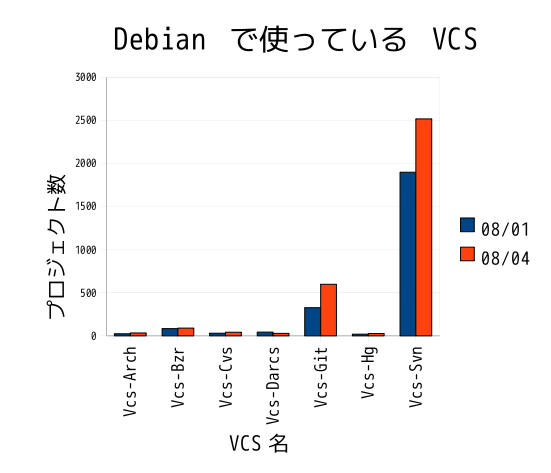
\includegraphics[width=0.5\hsize]{image200804/debian-vcs-200804.png}
\end{center}

\subsection{ソースパッケージをGit で管理するためのツール git-buildpackage}
\index{git-buildpackage} 
\index{git} 
\index{deb} 
では、実際に VCS を使って Debian Package を管理するためにはどのようにすればいいのでしょうか。
Debian パッケージを Git で管理するためのツールとして、git-buildpackage があります。
これを使うことによって、Git を使ってパッケージのソースコードを管理することができるようになります。
インストールはいつものとおり、{\bf apt-get} or {\bf aptitude} を使ってインストールする
ことが可能です。

\begin{commandline}
$sudo apt-get install git-buildpackage
\end{commandline}

\subsubsection{git-buildpackageで提供されるコマンド}
git-buildpackage で提供されるコマンドは表\ref{git-buildpackage-command}の4つしかありません。
これらのコマンドと Git コマンド を使って、パッケージのメンテナンスをすることになります。
Gitの細かい知識は必要ありませんが、基本的な使い方は知っておく必要があります。
   \begin{table}[h]
    \begin{center}
      {
        \begin{tabular}{l|l} \hline
                提供されるコマンド & 機能 \\ \hline \hline
/usr/bin/git-buildpackage & パッケージを作成する \\
/usr/bin/git-dch & Git のコミットログから Debian Changelog を作成する。\\
/usr/bin/git-import-dsc & 既存の Debian Package をGitにインポートする。\\
/usr/bin/git-import-orig & アップストリームからリリースされたソースコードをGitにインポートする。\\
           \end{tabular}
        }
     \caption{git-buildpackage で提供されるコマンド}
     \label{git-buildpackage-command}
    \end{center}
    \end{table}

\subsection{Gitの簡単な使い方}
表\ref{git-command}によく使う Git コマンドを紹介します。これだけ知っていれば、Gitを使った最低限の開発を行う
ことが可能です。
   \begin{table}[h]
    \begin{center}
      {
        \begin{tabular}{l|l} \hline
                Git コマンド(一部) & 機能 \\ \hline \hline
git init & ローカルリポジトリを作成する。\\
git add & ローカルリポジトリのキャッシュ(index)に管理対象のファイルを追加する。\\
git commit & ローカルリポジトリに変更を反映する。\\
git rm & ローカルリポジトリから管理対象ファイルを削除する。\\
git diff & 差分を取得する。\\
git branch & ブランチを作成する。\\
git checkout & 作成したブランチをチェックアウトする。\\
git format-patch & パッチを作成する。\\
           \end{tabular}
        }
     \caption{よく使うGitのコマンド}
     \label{git-command}
    \end{center}
    \end{table}

\subsection{既にパッケージ化されているものを Git で管理する}
Debian パッケージには2つの状態があると考えられます。一つは既にパッケージ化されているもの、
もうひとつは今からDebian パッケージにしようとしているものです。
まずは、既にDebian パッケージになっているものを Git で管理する方法を説明します。
\\

まず、git-import-dscコマンドを使い、Git リポジトリに現在のソースコードの状態を
取り込みます。コマンドのオプションに、パッケージの dscファイル\footnote{Debian パッケージの制御ファイル}
を指定します。実行すると、パッケージ名でディレクトリが作成され、Git リポジトリが作成されます。
また、ブランチとして、master ブランチと、upstream ブランチが作成されます。Debian 関係のコードは
 master 
ブランチ、Upstream のソースコードは upstream ブランチで管理されるようになります\footnote{ブランチは git branch コマンドで表示可能}。

\begin{commandline}
$ git-import-dsc ../isight-firmware-tools_1.0.2-1.dsc
Upstream version: 1.0.2
Debian version: 1
No git repository found, creating one.
Initialized empty Git repository in .git/
Everything imported under isight-firmware-tools
$ ls
isight-firmware-tools
$ cd isight-firmware-tools
$ git branch
* master
  upstream
\end{commandline}

\subsubsection{インポート時のログ}

パッケージをインポートしたときに、Git のコミットログに現在のバージョンのコミットログが書き込まれます。
また、 Debian Version は Git のタグ機能を使い、タグ名として保存されます。

\begin{commandline}
$ git log
commit 9c3669a233afe69d7be2aa8ad1995e6b19c841aa
Author: Nobuhiro Iwamatsu <iwamatsu@nigauri.org>
Date:   Sun Apr 6 21:48:40 2008 +0900

    Imported Debian patch 1.0.2-1
$ git tag
debian/1.0.2-1
upstream/1.0.2
\end{commandline}

\subsubsection{ソースコードを変更し、修正を管理する}

ソースコードを修正し、Debian パッケージ で配布する部分を管理するには、今までどおり、dpatchなどの
パッチ管理システムを使う必要があります。
作成したパッチをリポジトリにコミットする時にに、{\bf git add}, {\bf git commit} コマンドを使い、
リポジトリに反映させます。

\begin{commandline}
$ dpatch-edit-patch 05_change_ift-load_install_dir
... いろいろ修正 ...
$ exit
$ vi debian/patches/00list
$ git add debian/patches/05chage_ift-load_install_dir.dpatch
$ git commit -s debian/patches/00list debian/patches/05_chage_ift-load_install_dir.dpatch
/* エディタが起動するので、コミットログを記述 */

Change ift-load install dir.
    
Signed-off-by: Nobuhiro Iwamatsu <iwamatsu@nigauri.org>

$ git log
commit c9865153ae1949956fdfe3827c0da9b36c2f0ddb
Author: Nobuhiro Iwamatsu <iwamatsu@nigauri.org>
Date:   Sun Apr 6 21:23:20 2008 +0900

    Change ift-load install dir.
    
    Signed-off-by: Nobuhiro Iwamatsu <iwamatsu@nigauri.org>
\end{commandline}

\subsubsection{git-buildpackage を使ったDebian パッケージの作成}

Debian パッケージを作成するには、 git-buildpackage コマンドを使います。
--git-ignore-newオプションはGit に反映されていない修正を無視するための
オプションです。
\begin{commandline}
$ git-buildpackage --git-ignore-new -us -uc
\end{commandline}

\subsubsection{パッケージをリリースする}
新しい Debian バージョンのパッケージをリリースする場合は、{\bf git-dch} コマンドに
{\bf --release} オプションを付けます。実行することにより、エディタが立ち上がり、Git
のコミットログから、Debian Changelog が作成されます。
Changelog を作成したら、{\bf git-buildpackage} コマンドに {\bf--git-tag} オプションを
付けてパッケージを作成します。{\bf--git-tag} を付けると、リポジトリに Debian バージョン用の
タグが Debian changelog より作成され、リリース情報が付加されます。
\begin{commandline}
$ git-dch --release
$ git-buildpackage --git-ignore-new --git-tag
$ git tag
debian/1.0.2-1
debian/1.0.2-2
upstream/1.0.2
\end{commandline}

\subsubsection{新しいバージョンにする}
新しいバージョンにするには、git-import-orig コマンドを使い、リリースされた
新しいバージョンの Tar ボールを指定します。
指定することにより、ファイル名からバージョンを取得し、新たにUpstream 用の
タグが作成されます。
また、アップストリームのバージョンが上がるため、自動的に Debian Changelog に 次のDebian パッケージ
バージョンが追記されます。
\begin{commandline}
$ git-import-orig /tmp/isight-firmware-tools-1.2.tar.gz
Upstream version is 1.2.0
Importing '/tmp/isight-firmware-tools-1.2.tar.gz' to branch 'upstream'...
Switched to branch "upstream"
rm 'isight.rules.in'
rm 'po/fr_FR.po'
Created commit f5c85da: Imported Upstream version 1.2.0
 33 files changed, 4434 insertions(+), 1332 deletions(-)

.......<snip>

 src/udev.c                             |  164 +++
 33 files changed, 4434 insertions(+), 1332 deletions(-)
 rename po/{fr_FR.po => fr.po} (66%)
 create mode 100644 src/50-isight-firmware.fdi
 create mode 100644 src/callout.c
 create mode 100644 src/isight-firmware.fdi
 rename isight.rules.in => src/isight.rules.in (100%)
 create mode 100644 src/load.h
 create mode 100644 src/udev.c
Succesfully merged version 1.2 of /home/iwamatsu/Desktop/isight-firmware-tools-1.2.tar.gz into .
$ git branch
debian/1.0.2-1
debian/1.0.2-2
upstream/1.0.2
upstream/1.2
$ cat debian/changelog
isight-firmware-tools (1.2-1) unstable; urgency=low

  * New Upstream Version

 -- Nobuhiro Iwamatsu <iwamatsu@nigauri.org>  Fri, 11 Apr 2008 17:18:23 +0900

\end{commandline}

\subsection{新たにパッケージ化する場合}
新しくソフトウェアを Debian パッケージ にして、git-buildpackage で
管理する場合は 最初に Git の機能が必要です。
まず、ローカル Git リポジトリを作成します。次に作成したリポジトリに移動し、{\bf git-import-orig}
コマンドにアップストリームのソースコードを指定し、実行します。ソースコードは、gzip、bzip2 などで
圧縮されたものと、展開されたソースコードディレクトリを指定することが可能です。
また、実行する際に、{\bf-u} オプションで、アップストリームのバージョンを指定する事が可能です。
リポジトリを作成した後は upstream ブランチに移動し、{\bf dh\_make}等を使ってパッケージの雛形作成し、
上で説明した流れでメンテナンスを行います。

\begin{commandline}
$ mkdir isight-firmware-loader-1.2
$ cd isight-firmware-tools-1.2
$ git init /* ローカル Git リポジトリを作成する */
$ git-import-orig -u 1.2 /tmp/isight-firmware-tools-1.2.tar.gz /* ソースコードをコミット */
Upstream version is 1.2
Initial import of '/tmp/isight-firmware-tools-1.2.tar.gz' ...
Succesfully merged version 1.2 of /tmp/isight-firmware-tools-1.2.tar.gz into .
$ git log
commit 9bf014aee2f834576f8f03d67ab66e8c85726832
Author: Nobuhiro Iwamatsu <iwamatsu@nigauri.org>
Date:   Tue Apr 8 21:42:55 2008 +0900

    Imported Upstream version 1.2
$ git branch
* master
  upstream
$ git tag
upstream/1.2
$ git branch upsteam
$ dh_make
$ git branch master
\end{commandline}

%\subsubsection{git-buildpackage の設定 .git/gbp.conf}
%git-buildpackage は細かい設定を行うことが可能です。
%設定ファイルを .git ファイル


\dancersection{アップストリームの VCS と付き合う}{岩松 信洋}
\label{sec:upstreamvcs}
\index{vcs}
\index{git}
\index{upstream}
\index{あっぷすとりーむ@アップストリームのVCS}
% CVS / SVN / Git などの VCS をupstream が活用している場合の話。

VCS を使ってアップストリームがソフトウェアの開発を行っている事が多くあります。
アップストリームでは、Subversion を使っているが、パッケージメンテナは Git を使って
パッケージを行っている場合があったり、同じ VCS を使っている場合もあります。
今回は Subversion を例にして、お互い VCS を使っている場合、どのように付き合って
いくことができるのか説明します。

%\subsection{アップストリームが Git を使っている場合 }
%\subsection{アップストリームが CVS を使っている場合 }

\subsection{アップストリームが Subversion を使っている場合 }
Subversion で管理されているソースコードを取得したり、Subversion リポジトリへ
コミットするツールとして、git-svn パッケージがあります。 git-svn を使うことに
よって、容易に お互いのリポジトリ間を行き来することができるようになります。

\subsubsection{Subversion のリポジトリからGit のリポジトリへ ソースコードを取得する}
Subversion のリポジトリからGit のリポジトリへ ソースコードを取得するには
適当なディレクトリを作成し、 {\bf git svn} の {\bf clone} オプションを使って行います。
取得した後は、Git の操作で開発を行うことができます。

\begin{commandline}
$ mkdir test
$ git svn clone svn://test/trunk test-0.0.1
\end{commandline}

\subsection{取得したコードを元に Debian パッケージ を作成する}
取得したコードから新しく Debian パッケージ を作成するためには、自分でタグを付ける必要があります。
{\bf git-buildpackage}ではタグと Debian changelog から Upstream の情報を取得し、
orig.tar.gz 相当のものを作成するため、タグを付ける必要があります。

\begin{commandline}
$ git branch
master
$ git branch upstream
$ git checkout upstream
$ git tag upstream/0.0.1
$ dh_make --createorig
$ git branch master
.... Debian パッケージ 用のファイル作成などを行う ....
$ git-buildpackage -us -uc --git-ignore-new
$ debuild clean
$ git add debian
$ git commit -a
$ git-buildpackage -us -uc --git-ignore-new --git-tag
\end{commandline}


\subsubsection{Subversion リポジトリの情報を取得する}
Subversion リポジトリの情報を取得するには、 {\bf rebase}オプションを使います。
最初から git svn でリポジトリの操作を行っている場合は、rebase を使うことにより、
Upstream のコードを パッケージ側に反映させることができます。
\begin{commandline}
$ git checkout upstream
$ git svn rebase
\end{commandline}

\subsection{すでにあるパッケージと Git リポジトリを元に Debian パッケージ を作成する}

\begin{minipage}{0.5\hsize}
{\bf git svn} で取得したGit リポジトリと 既にあるDebian パッケージ を連携させるには
操作が少し必要です。
まず、{\bf git-import-dsc}で 現在の Debian パッケージ を git-buildpackage で管理できる
ようにした後、upstream ブランチに git svn で取得したリポジトリから pull をします。
pull することにより、コミットログの共有することができます。
しかし、Debian Changelog の操作や、{\bf git tag} を使ったタグの操作を手動で行う必要がある
のが問題点です。
{\bf git-import-orig } を使って、tar.gz や ソースコードを指定して、マージすることも可能ですが、
Upstream 側のコミットログが取り込まれないため、 Gitを使うメリットがあまり無いと私は考えています。
このあたりを改善していく事が今後の課題になりそうです。
\end{minipage}
\begin{minipage}{0.5\hsize}
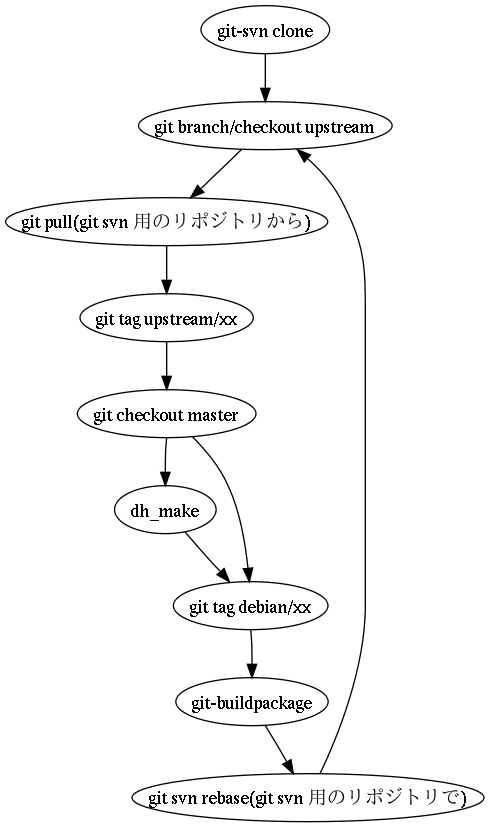
\includegraphics[width=0.8\hsize]{image200804/git-svn_with_build-package.png}
\end{minipage}

\begin{commandline}
$ git svn clone svn://svn.berlios.de/linux-uvc/linux-uvc/trunk\
 linux-uvc.git
$ git import-dsc  ../../../debian/linux-uvc_0.1.0.svn193-2.dsc
$ cd linux-uvc
$ git branch
* master
  upstream
$ git tag
debian/0.1.0.svn193-2
upstream/0.1.0.svn193
$ git checkout upstream
$ git pull ../linux-uvc.git/
$ git tag upstream/0.1.0.svn201
$ git checkout master
$ dch -v 0.1.0.svn201
$ git-buildpackage -us -uc --git-ignore-new
$ debuild clean
$ git commit -a
$ git-buildpackage -us -uc --git-ignore-new --git-tag
\end{commandline}



\dancersection{東京エリアDebian勉強会の設計}{上川 純一}
\label{sec:debmtg2007design}

\index{debianjp@Debian JP} 
\index{とうきょうえりあ@東京エリアDebian勉強会}

Debian勉強会はDebianの日本における発展を支援するために実施しているイベン
トです。Debian勉強会を運営している上での仮説を説明します。勉強会はこの仮
説に基づいて運営しています。まず前提条件を整理したのち、現状の状況を分析
して、Debian勉強会からどういう成果が期待できるのかを整理します。

\subsection{Debian JP とは}

Debian Project メンバーの日本在住の有志およびDebian Projectの Debian
Developer になる候補者で構成されているのがDebian 開発者の会(Debian JP)
です。Debian JP の会員はどういう人が存在しているのか、という点を議論した
ところ、下記の分類があぶり出されました。

\begin{itemize}
 \item Debian JPの会員は開発・翻訳・インフラを担当している人により構成さ
	れています。過去の経緯により、既存の会則・方針では、Debian JP は
	「開発者の会」という位置づけのため、「ユーザ」については Debian
	JP 「会員\footnote{Debian 開発者の会の「会員」は会則に定義されて
       おり、例えば投票する義務のある人のことです}」ではありません。
 \item 開発者とは Debian JP で開発を行っている人、パッケージ・スポンサー
	されている人、New Maintainer、 Debian Developer などをいいます。
 \item インフラは、Debian JP の運営に必要なインフラで ftp, www, svn, ML,
       LDAP などをいいます。
\end{itemize}

\begin{figure}[h]
\begin{center}
  {\large
 \begin{tabular}[t]{|c|c|c|}
 \hline
 \rotatebox{90}{ユーザ }& \rotatebox{90}{開発者 }&\rotatebox{90}{翻訳者 } \\
 \hline 
 \multicolumn{3}{|c|}{インフラ}\\
 \hline
 \end{tabular}
 }
\end{center}
 \caption{Debian JP のメンバー要素分類}
\label{fig:debianjpmemberitem}
\end{figure}

Debian JP の目的としては、いろいろありますが、Debianの日本の開発者
(Debian Developer)のコミュニティーとなることを目指しています。また日本
におけるDebianの代表・とりまとめとしての役割をになっており、Debianが日本
で利用しやすくなることの促進を行っており、翻訳作業のとりまとめや、外国か
らDebian Developerが来訪したときの宴会調整の連絡先として機能していたりし
ます。また、Debianの商標を管理していたりします。



Debian JP が成功すると、Debianの日本語対応がよくなり、日本にいるDebian
Developerがふえ、日本にいるDebianユーザがふえ、日本でDebianを使うことがや
りやすくなるはずです。

Debian JP の目的から考えると、開発者のコミュニティーとしての機能、および
ユーザとの情報交換の機能の部分を保管するのが東京エリアDebian勉強会でしょ
う。また、今後のDebian Developer候補の発掘・育成(・そそのかし)のために
活動すればよいでしょう。




\subsection{Debian JP の各種会議体の位置付け}

Debian Projectには各種組織、および会議体が存在します。東京エリア Debian
勉強会を中心に、それらの関係を整理してみます。

「東京エリア Debian 勉強会」はDebian Projectの日本における組織である
Debian JP が主体となり、「東京エリア Debian 勉強会幹事」に委任して開催し
ているイベントです。目的としているのは、Debianのパワーユーザと既存の開発
者層に着目し、Debian Developerの育成、および翻訳活動に参加できる人たちへ
の情報提供、および必要な情報の交換です。

\includegraphics[width=1\hsize]{image200712/debianmeetinganddebianjp.eps}

各種定期的に開催している会議体を整理してみます。

\begin{tabular}[t]{|l|l|p{14em}|p{12em}|}
\hline
会 & 開催頻度 & 目的 & 参加者層 \\
\hline
総会・選挙 & 年一回 & Debian JP 内部の運営方針の策定 & Debian JP 会員 \\
OSC & 年数回 & 新規ユーザ発掘・公報 & OSCの一般参加者 \\
東京エリアDebian勉強会 & 月一回 & Debian 開発者の新規発掘と支援 & Debian の開発者をめざす東京近辺在住の
 メンバー \\
関西Debian勉強会 & 月一回 & Debian ユーザ・開発者の新規発掘と支援 & Debian を使う大阪近辺
	     在住のメンバー\\
IRC定例会議 & 月に二回程度 & Debian JPの運営に関する情報共有と意思決定 & Debian JP
 会員 \\
\hline
\end{tabular}

会議の情報が伝達される経路について整理してみます。Debian JPで
利用している主な情報交換の方法を整理してみました。各種の会議が開催され、
成果が報告されます。参加したメンバーが情報を得られるのはもちろんですが、
参加していないメンバーもなんらかの情報が取得できます。事前資料は公開され
るため、ウェブで取得できます。また、その他の情報取得の手段があります。

\includegraphics[width=1\hsize]{image200712/debianjpandmedia.eps}


\subsection{東京エリアDebian勉強会においての事前資料の意義}

「事前資料」は記録性、参照性を重視しています。2007年12月の「事前資料」は
当日の勉強会でも利用しますが、今年の勉強会の幹事・講師をしてくれる人の説
明資料としても随時利用します。「これを読めば何をすればよいかがわかる」と
いう形にしたいと思っています。プレゼンテーションに利用する資料は若干毛色
が違い、議論をするためのフレームワークを提供するものだと考えています。

「事前資料」については、勉強会で紙の媒体の資料として利用するのと、コミッ
クマーケットを契機として「あんどきゅめんてっど でびあん」として再度編集
し、半年に一度まとめて製本します。そのことで、知識の精査、定着と展開がは
かれることを目的としています。

\subsection{事前課題の役割}

東京エリア Debian 勉強会では、ただのセミナー参加でおわることは期待してい
ません。理想的な最終目標としては、Debian Developer としてばりばりと貢献で
きるような意識の高い参加者を求めています。そこまでの理想を追い求めるのは
現実的ではないにしても、何も準備せずに参加するより、何らかの心構えをして
参加してもらった方がよいだろうということで、毎回事前課題を設定しています。
いろいろなアイデアが出てきておもしろいです。

参加する際には事前課題は必須ということにしています。今年の参加者の事前課
題の提出率を見ると半分以上が提出していることが分かります。

\begin{table}[h]
 \caption{2007年の事前課題}
 \begin{center} 
  \begin{tabular}{|l|c|c|p{20em}|}
 \hline
 & 参加人数 & 事前課題提出人数 & 内容\\
 \hline
 2007年1月 & 15 & 6 & 今後、勉強会につかう施設を提案してください、2007年の勉強会の各月のアジェンダを提案してください\\
 2007年2月 & 13 & 8 & aptに足りなさそうな機能, パッケージングをしてみて感じたこと、または何故パッケージングをしないか\\
 2007年3月 & 80 & 6 & 仮想化を実際にこういう利用方法で活用しています\\
 2007年4月 & 19 & 14 & 私はバージョン管理システムをこのようにつかっています \\ 
 2007年5月 & 23 & 14 & 「エッチになって困った事」 \\
 2007年6月 & 4 & & \\
 2007年7月 & 18 & 12 & 今後Debconfを日本で開催するためにDebianの認知度を上げる方法、企業がDebconfのスポンサーになるためには \\
 2007年8月 & 25 & 18 & ここ最近 Debian を使っていて ハマったこと/ちょっと
	       感激したこと、apt の sources.list はこう書く\\
 2007年9月 & 14 & 7 & 「あなたがDebianで使っている MTA のこだわりの設定」もしくは「Debian 
 で利用しているこんな便利な/楽しいメッセージツールあるいは日頃使っていて
 気にかかるメッセージ関連ソフトのこの部分」\\
 2007年10月 & 30 & & \\
 2007年11月 & 19 & 10 & 「Debian の Live CD ってこんなふうに使ってます」もしく
	   は「ノートPCやデスクトップPCではなく、サーバ機器での Debian
	   に期待するものって何?」\\
 2007年12月 & 11 & 11 & 「Debian勉強会の目的と照らし合わせて2007年を評価してみた」と「2008年のDebian勉強会のために私はこうします」 \\
 \hline
  \end{tabular}
 \end{center}
\end{table}

\subsection{12月の勉強会の役割}

毎年の忘年会をかねて東京エリアDebian勉強会の12月開催は、一年間を反省する
会を開催しています。12月号の事前資料は、運営に関連する情報を共有するため
に準備しています。ターゲットは幹事・講師で、その説明文を見ることで講師や
幹事が何をどういう理由で実施する必要があるのかを理解できることを目的とし
ています。内容については定期的に修正が必要なものなので、毎年12月の資料と
して新規に作成しています。勉強会の目的は通常と違い、勉強会の実績の確認と、
今後の方向性の策定だけをするという会にしています。

\dancersection{東京エリア Debian 勉強会のワークフロー}{上川 純一}
\label{sec:debmtg2007workflow}
\index{debianjp@Debian JP} 
\index{とうきょうえりあ@東京エリアDebian勉強会}

東京エリア Debian 勉強会は事前に会場も日時も決定してしまっています、その
ため資料の準備・告知・予約などができる期限が決まっています。Debian 勉強会
では月に二回行われる Debian JP IRC 定例会議と、幹事用のメーリングリストを
利用して進捗の管理をしています。開催直前の最後の一週間はタイトになります。
ワークフローの内容をみてみましょう。git レポジトリの
\url{planner/200704-tokyo.ods} にファイルが置いてあります。

毎月の作業は次のようなものがあります。
\begin{description}
\item[会場確保]  勉強会の会場を予約します。2ヶ月前程度に予約しないと大抵
	   の会場はうまってしまいます。日程については年間スケジュールを
	   事前に確定しておき、それから若干の調整をかける形にするのがよ
	   いでしょう。
\item[企画立案] 企画を立案します。前回の勉強会の宴会、もしくは年初の企画
	   会議などで決定します。
\item[講師確保] 前回の勉強会であたりをつけて、講師候補のメールで調整する
	   ようにします。
\item[資料作成依頼] 資料の作成を講師に依頼します。資料の作成の方法につい
	   ての資料も必要でしょう。
\item[資料作成] 講師が資料を作成します。git レポジトリを活用して共同作業
	   をするのがよいでしょう。
\item[資料編集] 資料を集めて資料を編集します。元の資料が \LaTeX{}でない
	   場合には\LaTeX{}形式にする作業などがあります。ページ数にあて
	   はまるようにする、用語を統一する、誤字脱字を修正する、などの
	   対応を行います。
\item[印刷向け編集(4の倍数)] 冊子として印刷に出すときに紙は4ページの
	   倍数である必要があります。そのために技を駆使します。内容をけ
	   ずったり、画像の位置を微調整したり、フォントを小さくしたり、
	   文章が一行におさまるように書き直したり、などの技があるようで
	   す。
\item[kinkos印刷依頼] kinkos に印刷を依頼します。ウェブ経由でお願いする
	   ことができます。\url{http://www.kinkos.co.jp/}からアクセスし
	   て、「オンラインプリント」のメニューを選択します。半日程度
	   (12時間)は余裕をみてあげるのがよいでしょう。
\item[kinkos印刷受け取り] 印刷したものを受け取ります。面倒ですが、確認の
	   意味も含めて、直接うけとって支払
	   うのがよいでしょう。
\item[事前課題設定] 参加者に事前に考えてきてほしい内容を設定します。勉強
	   会の次回の企画テーマにあうようなものがよいです。またハードル
	   が高すぎると参加者がこまっちゃうので気を付けましょう。
\item[事前課題提示] 事前課題をウェブページに提示します。
\item[資料反映] 資料を反映します。
\item[DWN Quiz作成] クイズを作成します。わからないとどうしようもないので、
	   わかりやすいものをこころがけましょう。
\item[DWN Quiz景品準備] 何か景品を準備しましょう。
\item[案内文文書案作成] 案内文の素案を作成します。見た人が参加したくなる
	   ように、また参加して意味のある人が参加できるように、何を期待
	   したらよいかを明確にします。これは幹事MLでレビューにまわしま
	   す。
\item[案内文確定] レビューした後、案内文を確定します。各種メディアに展開
	   します。
\item[aliothウェブ掲載] alioth のウェブページに掲載します。
\item[debian.or.jp掲載] debian.or.jp のウェブページに掲載します。
	   掲載の方法については
	   \url{http://www.debian.or.jp/community/translate/webmasters.html}
	   を参照。
	   \texttt{www/trunk/src/community/events/index.tt2} のイベント
	   の一覧に追加し、 \texttt{www/trunk/blosxom/data/} に blog エントリーを追加
	   します。
\item[mixi掲載]  mixi の debian コミュニティーに掲載します。\url{http://mixi.jp/view_community.pl?id=95}
\item[debian-devel投稿]
	   Debian JPのメーリングリスト \url{debian-devel@debian.or.jp},
	   \url{debian-users@debian.or.jp} に投稿します。
	   二週間前ごろをメドにします。
\item[debian-devel再度投稿]
	   数日前に再度投稿します。
\item[予約システムの作成]
	   宴会くん \url{http://utage.org/enkai/}などを利用し、
	   予約用のエントリーを作成します。これは3週間前くらいにはつくっ
	   ておきます。
	   
\item[参加者把握]
	   数日前に参加者を把握しておきます。
\item[出席簿印刷]
	   当日のために出席簿を印刷します。
\item[宴会予約]
	   宴会の場所を予約します。場所によりますが前日までに予約したほ
	   うがよいです。店に電話で直接連絡します。
\item[宴会費回収] 宴会を開催、代金を回収します。5000円、4000円などのきり
	   のよい金額が会費として徴収できるように調整します。東京Debian
	   勉強会では講師をしてくれた人に関しては徴収しないようにしてい
	   ます。
\item[会場設置] 会場を設置します。事前に幹事がはやめに入ることが必要です。
	   一人ではできないので、手伝ってくれる人がきてくれないと困るな。
\item[出席確認] 会費を徴収し、資料を配布します。受付担当者としては、参加
	   者の方の名前を覚えるチャンスです。
\item[結果報告書整理] 
	   実際に今回どういう会だったのかということを整理し、報告にまと
	   めます。
	   \url{http://tokyodebian.alioth.debian.org/}
	   ウェブページから反応リンク集という形でまとめ、
	   Debian JP IRC会議にて内容を報告します。
\end{description}

年間一度している作業内容は次のようなものがあります。
\begin{description}
\item[年間スケジュール設定] 一年間のスケジュールを決定します。内容につい
	   てはあまり重要ではありませんが、会場の予約のためには日程が決
	   まっていることが重要です。
\item[前年度の内容確認] 出席者の傾向、開催内容の傾向と参加者数の増減、
	   Debian JPの傾向などを分析し、どういう状況で、何が行われたのか、
	   を確認します。
\item[tokyodebian-XXX ML作成] 事前課題を投稿してもらっているメーリングリ
	   ストを再設定します。
\end{description}


\dancersection{東京エリア Debian 勉強会資料の準備の方法}{上川 純一}
\label{sec:debmtg2007howtoprepare}
\index{debianjp@Debian JP} 
\index{とうきょうえりあ@東京エリアDebian勉強会}

\subsection{文章ルール}

文章は敬体に統一しましょう。

固有名詞は基本としては敬称略、フルネーム、で記述しましょう。日本名称の場
合、苗字と名前の間には半角の空白を一文字入れます。

\subsection{レポジトリの取得}

まず最初にgitのレポジトリを取得します\footnote{git の使いかた詳細につい
ては、2007年4月の勉強会資料を参照してください。 apt-get install git-core
でインストールできます。} 。読み込み専用であれば、
git プロトコル、もしくは、http プロトコルでよいでしょう。書き込み権限を
持っているのであれば、ssh プロトコルを利用すれば直接 git push でアクセス
することができます。


\begin{commandline}
 git clone git://git.debian.org/git/tokyodebian/monthly-report.git
 git clone http://git.debian.org/git/tokyodebian/monthly-report.git
 git clone ssh://git.debian.org/git/tokyodebian/monthly-report.git
\end{commandline}

この結果、カレントディレクトリに monthly-report というディレクトリができ
ます。
monthly-report/.git 以下がレポジトリです。
git の使いかたについては 4 月の資料を参照してください。

\begin{commandline}
$ ls -la monthly-report/ | head
合計 2500
drwxr-xr-x 28 dancer dancer   1960 2007-04-22 09:46 .
drwxrwxrwt 17 root   root      560 2007-04-22 09:46 ..
-rw-r--r--  1 dancer dancer    168 2007-04-22 09:46 .cvsignore
drwxr-xr-x  8 dancer dancer    240 2007-04-22 09:46 .git
-rw-r--r--  1 dancer dancer     61 2007-04-22 09:46 .gitignore
-rw-r--r--  1 dancer dancer     71 2007-04-22 09:46 .whizzytexrc
-rw-r--r--  1 dancer dancer    145 2007-04-22 09:46 .yatexrc
-rw-r--r--  1 dancer dancer  17989 2007-04-22 09:46 COPYING
-rw-r--r--  1 dancer dancer  25069 2007-04-22 09:46 ChangeLog
\end{commandline}
%$

\subsection{コミットの方法}

まず、PDFファイルが生成できることを確認します。Makefile があるので、make 
コマンドを入力するとビルドしてくれるはずです。
文字コードが正しいか、正常にビルドできるか、などのチェックが組み込まれて
いるので、チェックに活用しましょう。

\begin{commandline}
 make
\end{commandline}

その後、git diffでコミットされる内容を確認します。意図している内容が表示
され、問題ないようであれば、git commit コマンドでコミットします。手元のレ
ポジトリに反映されます。

\begin{commandline}
 git diff
 git commit -a -m 'revised XXX'
\end{commandline}

問題がないようであれば、git pull / git push でマージします。git pull し
た後にコンフリクトが発生したら、修正し、git commit でコミットしてから
git push します。

\begin{commandline}
 git pull 
 git push 
\end{commandline}

新規のファイルを追加する場合、ファイルを削除する場合には、 git add /
git rm コマンドを利用します。

\subsection{ファイルの編集}

\index{latex@\LaTeX}
ドキュメントは p\LaTeX{}で作成しています。ファイル名として下記になってい
ます。(YYYY)(MM)は、年と月で、例えば2007年12月であれば 200712 です。

\begin{description}
 \item[debianmeetingresume(YYYY)(MM).tex]
	    事前配布資料
 \item[debianmeetingresume(YYYY)(MM)-presentation.tex]
	    プレゼンテーション用 (prosperを利用)
 \item[image(YYYY)(MM)/]
	    画像ファイルなどの置き場
\end{description}


作業する前にビルドに必要なパッケージをインストールします。

\begin{commandline}
# tex から PDF の生成関連
apt-get install ptex-bin dvipdfmx latex-beamer \
 okumura-clsfiles gs-esp xpdf xpdf-japanese
\end{commandline}

編集に便利なツールもついでにインストールしてみてもよいでしょう。

\begin{commandline}
 apt-get install whizzytex advi emacs21 yatex gs-cjk-resource gv
\end{commandline}

tex4ht を利用して HTML 出力をさせる場合は下記もインストールしたらよいで
しょう。ただし、2007年8月現在、dvi2ps-fontdata-a2n の影響で dvi 出力ができなくな
る副作用があります。

\begin{commandline}

# tex4ht での HTML 生成関連
apt-get install dvi2ps-fontdata-a2n dvi2dvi dvipng tex4ht
\end{commandline}

文字コードは iso-2022-jp で統一しています\footnote{Windows 版と Linux 版
の ptex で共通して扱える文字コードにしたという経緯があります。ただし現状
Windows で全部できる状況ではありません。}。たとえば、emacs + yatex を使用
している場合で iso-2022-jp をデフォルトにするには、下記のような設定を
\texttt{.emacs} にかけばよいでしょう。

\begin{commandline}
(add-hook 'yatex-mode-hook
	  '(lambda () 
	     (progn 
	       (if (string-match "^/home/user/tokyodebian/" default-directory)
		   (progn (set-buffer-file-coding-system 'iso-2022-jp)
			  (set-buffer-modified-p nil))))))
\end{commandline}


emacs での編集で、outline-mode を利用すると、アウトラインをベースに編集す
ることができ、便利です。tex ファイルの最後に以下のようなエントリーを追加
しています。
M-x outline-minor-mode で有効にできます。

\begin{commandline}
;;; Local Variables: ***
;;; outline-regexp: "\\([ <タブ記号>]*\\\\\\(documentstyle\\|documentclass\\|<改行しない>
dancersection\\)\\*?[ <タブ記号>]*[[{]\\|[%<^L>]+\\)" ***
;;; End: ***
\end{commandline}

\begin{itemize}
 \item 
 \verb!<タブ記号>!: タブを入力、
 \item  \verb!<^L>!: ctrl-L を入力、
 \item  \verb!<改行しない>!: ここの改行はみやすいように改行をいれているだけで、実際には改行は入力しない。
\end{itemize}

また、自動で適切な設定で outline-minor-mode に入るように .emacs に設定してもよいでしょう。

\begin{commandline}
(add-hook 
 'yatex-mode-hook
 '(lambda ()
    (make-variable-buffer-local 'outline-regexp)
    (setq outline-regexp 
	  "\\([ \t]*\\\\\\(documentstyle\\|documentclass\\|chapter\\|dancersection\\|
section\\|subsection\\|subsubsection\\|paragraph\\)\\*?[ \t]*[[{]\\|[%\f]+\\)")
    (setq 
     outline-level 
     (function
      (lambda ()
	(save-excursion
		   (looking-at outline-regexp)
		   (cond 
		    ((equal (char-after (match-beginning 0)) 37) (- (match-end 0) (match-beginning 0)))
		    (t (let ((bs (buffer-substring (match-beginning 2) (match-end 2))))
			 (cond ((equal (substring bs 0 2) "do") 15)
			       ((equal (substring bs 0 1) "c") 0)
			       ((equal (substring bs 0 1) "p") 4)
			       ((equal (substring bs 0 2) "da") 1) ; dancersection
			       ((equal (substring bs 0 2) "se") 1) ;section
			       ((equal (substring bs 0 5) "subse") 2) ;subsection
			       ((equal (substring bs 0 8) "subsubse") 3) ;subsubsection
			       (t (length bs))))))))))
    (outline-minor-mode t)))
\end{commandline}

\subsubsection{ドキュメントのスタイル}

スタイルファイルは monthlyreport.sty パッケージを利用します。過去の資料を参考にしてください。

\begin{commandline}
\usepackage{monthlyreport} 
\end{commandline}

各担当部分は section として扱います。特別なコマンド dancersection で指定
します。形式は \texttt{\textbackslash{}dancersecion\{タイトル\}\{作者名\}}です。
その中で subsection や subsubsection を利用して文書を構成してくださ
い。

\begin{commandline}
 \dancersection{Debian 勉強会資料の準備の方法}{上川 純一}
 \label{sec:debmtg2007howtoprepare}
\end{commandline}

\subsubsection{目次の処理}

目次のエントリは下記の形式で作成します。
\begin{commandline}
\index { alphabet もしくは、 ひらがなの読み @ 項目名称 } 
\end{commandline}

\subsubsection{画像ファイルの処理}

画面写真の画像を追加するときは、できるだけサイズの小さい png などを利用
してください。グラフなどの線画であれば、epsでかまいません。png であれば、 
ebb コマンドを利用してbounding box を作成してください。

\begin{commandline}
 ebb XXX.png
\end{commandline}

ps であれば、 eps2epsでバウンディングボックスを追加してあげるとうまくい
きます。sodipodi の出力する ps を eps2epsで処理すれば sodipodi で画像を
作成することができます。

\subsection{pLaTeX+latex-beamerで文書作成}

latex-beamer で生成したファイルは現状 whizzytex+advi でプリビューできませ
んが、gv, もしくは xpdf を利用してプリビューすることは可能です。
latexソースファイルの最初の行のコメント部分に特殊な文字列を記述すること
でwhizzytexは設定可能です。
そこで、gv を利用する場合は ps モードを指定します。
advi を利用しているときのように自動で編集しているページに飛んだりはしま
せんが、自動リビルド、および自動更新がかかるよういなります。

\begin{commandline}
 %; whizzy document -ps gv
\end{commandline}

xpdf を利用する場合は次のように設定します。

\begin{commandline}
 %; whizzy section -pdf xpdf -latex ./whizzypdfptex.sh
\end{commandline}

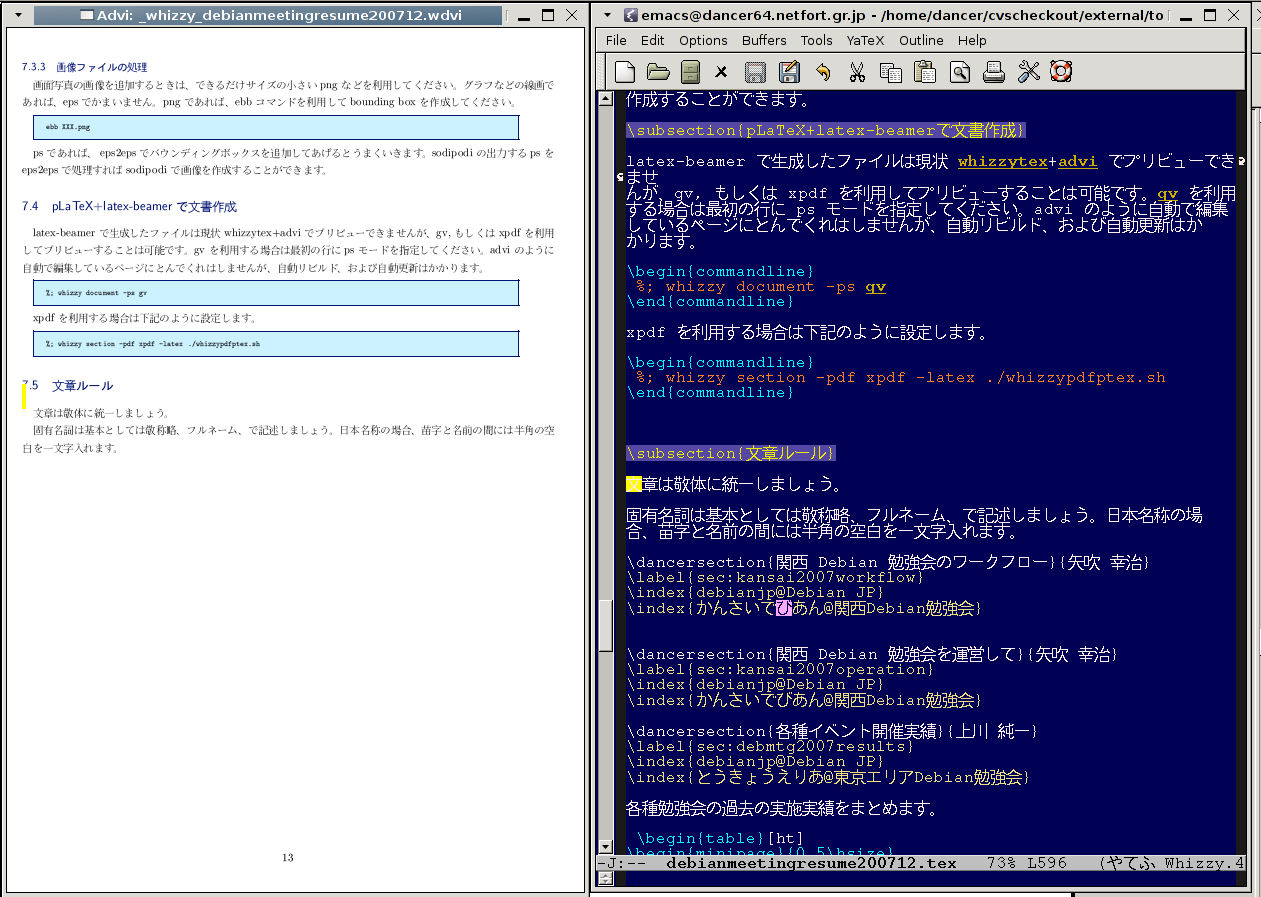
\includegraphics[width=1\hsize]{image200712/whizzytex.png}

\dancersection{関西 Debian 勉強会}{山下 尊也}
\label{sec:kansai2007operation}
\index{debianjp@Debian JP} 
\index{かんさいでびあん@関西Debian勉強会}

\subsection{関西 Debian 勉強会を運営して}

2007年の1年間、いろいろな人の支えがあって勉強会が成立したのだというのが、
2007年12月の忘年会が終わった後の私の率直な感想です。
9月に矢吹さんから私に担当が変わり、最初は運営の方でかなり悩んでいました。
だって、宴会の幹事とかやった事がない20歳になったばかりの担当者ですから。
しかし、回を重ね、それらは宴会などで運営についての会話を続ける事により、
お互いが理解出来る状態になれたと思います。そのため、来年の目標は、「長続
きできる勉強会」と言うテーマで運営していきます。

一人の力で運営を行うと、その一人が忙しくなった場合などに対応できず、バト
ンパスさえも難しい状況に陥ります。しかし、日頃から分
担して作業を行なっていれば、これからも継続出きるでしょう。

また、Debianについてもっと知りたいと言う事で、関西Debian勉強会の有志で
関西Debian勉強会とは独立した形で、週に一度、読書会(KDR)を開いています。
東京と色は違いますが、関西なりの色で私たち関西Debian勉強会は、より多く
Debianを愛する人で集い、勉強し、お互いが成長出来る勉強会にしたいと考えて
います。

\subsection{関西 Debian 勉強会のワークフロー}

では、感想を述べたところで、実際のワークフローについて紹介します。

関西Debian勉強会では、東京エリアDebian勉強会と同様に、Debian JP の IRC定
例会議に参加し、報告はしていますが、IRC 会議に出れる関西Debian勉強会のメ
ンバーが少ないため、主に幹事用のメーリングリストを利用して進捗の管理をし
ています。まだ、確立出来てない部分もあり、最後の一週間はとてもタイトにな
ります。この一年で関西なりに工夫したワークフローです。東京のワークフロー
を参考に作成しました。関西Debian勉強会では、共有作業の利便性の面でGoogle
ドキュメントで管理しています。

\begin{description}
\item[会場確保] ほとんどの会場は、3ヶ月前から予約の受付が始まります。
	   関西Debian勉強会は土日の午後を予約するため、2ヶ月前にはほとんど
	   の場所が予約で埋まってしまいます。そのため、企画が決定するより前に会場
	   を確保します。会場の料金支払いについては、前日までに入金すれば良いなど比較
	   的融通効くので、とりあえず会場を確保します。また、プロジェ
	   クターを利用する場合は会場確保の段階で伝えておかないと、当日
	   借りる事が出来ない場合もあります。気をつけましょう。
\item[企画立案] 企画を立案します。前回の勉強会の宴会で大抵決定します。12
	   月の忘年会で、どこらへんでお願いするかなどをお願いしておきます。
\item[講師確保] 前回の勉強会の宴会であたりをつけて、講師候補のメールで調
	   整するようにします。
\item[資料作成依頼] 資料の作成を講師に依頼します。
\item[資料作成] 講師が資料を作成します。
\item[資料編集] 資料を集めて資料を編集します。関西Debian勉強会では、講師
	   の負担を軽減するため、\LaTeX{}に限定はしておりません。そのた
	   め、OpenOfficeでの提出も可能です。
\item[印刷向け編集] 利便性の向上のため、PDFで結合します。
	   pdftk\footnote{\url{http://packages.debian.org/sid/pdftk}}などを使
	   うと良いでしょう。
\item[印刷] kinkos\footnote{\url{http://www.kinkos.co.jp/}} やカンプリ
	   \footnote{\url{http://www.kanpuri.co.jp/}}などの業者さんに持って行
	   きます。カンプリの場合は、メンバー割引があり、kinkosの場合は、
	   学生割引があります。開催者側の予定が合わない場合は、kinkosに
	   Webから印刷を依頼する事をを検討しても良いかもしれません。
\item[事前課題設定] 関西Debian勉強会では、基本的に参加者の敷居を下げるために事前課題
	   の設定はしておりません。ただし、希望などがある際は、MLで相談して事前
	   課題を設定します。
\item[事前課題提示] 事前課題をWikiに提示します。
\item[資料反映] 資料に反映します。
\item[案内文文章案作成] 案内文の作成をします。文面は前回の勉強会の時に使っ
	   たものを再利用して加工したものに対してMLで手直しを依頼します。
\item[案内文確定] 手直しなどがなくなったら、案内文を確定します。
\item[mixi掲載] mixiのdebianコミュニティ\footnote{\url{http://mixi.jp/view_community.pl?id=95}}と、
Debian初心者!コミュニティ\footnote{\url{http://mixi.jp/view_community.pl?id=958407}}
に投げます。また、女性のLinux使いコミュニティ\footnote{\url{http://mixi.jp/view_community.pl?id=513105}}に投げてもらうために、女性の方に依頼します。
\item[イベント管理システムの作成] 参加者が参加申し込みのためのフォームを
	   作成します。cotocoto京都\footnote{\url{http://cotocoto.jp}}などを利用し、
	   debian-users,debian-develに投稿する前には作成しておきます。
\item[debian-users,debian-devel投稿] Debian JPのメーリングリスト\footnote{\url{debian-users@debian.or.jp},\url{debian-devel@debian.or.jp},}
に投稿します。二週間前ごろをメドにします。
\item[debian-users,debian-devel再度投稿] 一週間前ごろをメドにします。ここ
で変更すべき内容は変更を行い、当日の予定とします。
\item[DebianJPページ] DebianJP会員が、DebianJPのイベントのページを更新します。
\item[参加者把握] 数日前に参加者を把握しておきます。
\item[出席簿印刷] 当日か前日に出席簿を印刷します。
\item[宴会予約] 宴会の場所を予約します。店に電話で直接連絡します。
最近の参加者の意見として、4000円以内に収まる事が望ましいみたいです。
\item[宴会費回収] 宴会の最後に、代金を回収します。
関西Debian勉強会では、講師の方と学生については1000円引きを実施しています。
\item[会場設置] 事前に幹事がはやめに入ることが必要です。
開始時刻よりも前から会場を取っているので、30分ほど前には集まり、会場を設
置します。
\item[出席確認] 出席を確認します。幹事と講師はプロジェクターの設置などで忙しいため、それ
以外の方にやっていただきます。
\item[結果報告書整理] Debian wiki\footnote{\url{http://www.debian.org}}の
	   関西Debian勉強会のページに反応集があるので、そこに記述を行いま
	   す。まだ Debian Wiki のアカウントを持っていない方は、今後のた
	   めに、アカウントを取っておきましょう。また、結果はDebianJP定例
	   会議や、次の勉強会で発表します。
\item[資料公開] Debian wiki\footnote{\url{http://www.debian.org}}の関西Debian
	   勉強会のページに資料を公開します。
\end{description}

\dancersection{各種イベント開催実績}{上川 純一}
\label{sec:debmtg2007results}
\index{debianjp@Debian JP} 
\index{とうきょうえりあ@東京エリアDebian勉強会}

各種勉強会の過去の実施実績をまとめます。
東京エリアDebian勉強会と、関西Debian勉強会について整理します。
グラフにしてみると\fgref{fig:peoplechart}になります。
\begin{figure}[h]
 \begin{center}
  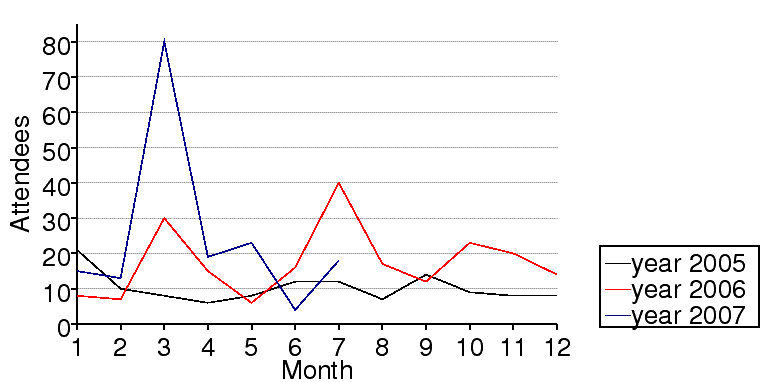
\includegraphics[width=12cm]{image200712/people-chart.png}
 \end{center}
\caption{参加人数推移}
\label{fig:peoplechart}
\end{figure}

表で見てみましょう。
 
 \begin{table}[ht]
\begin{minipage}{0.5\hsize}
 \caption{東京エリアDebian勉強会参加人数(2005年)}\label{tab:count}
 \begin{center}
  \begin{tabular}{|l|c|p{10em}|}
 \hline
   & 人数 & 内容 \\
 \hline
   2005年1月 & 21 & 秘密\\
   2005年2月 & 10 & debhelper1\\
   2005年3月 & 8 &  (早朝) debhelper2、social contract\\
   2005年4月 & 6 & debhelper3\\
   2005年5月 & 8 & DFSG、dpkg-cross、lintian/linda\\
   2005年6月 & 12 & alternatives、d-i\\
   2005年7月 & 12 & toolchain、dpatch\\
   2005年8月 & 7 & Debconf参加報告、ITPからアップロードまで\\
   2005年9月 & 14 & debconf\\
   2005年10月 & 9 & apt-listbugs、バグレポート、debconf翻訳、debbugs\\
   2005年11月 & 8 & DWN翻訳フロー、statoverride\\
   2005年12月 & 8 & 忘年会\\
 \hline
  \end{tabular}
 \end{center}
\end{minipage}
\begin{minipage}{0.5\hsize}
 \caption{東京エリアDebian勉強会参加人数(2006年)}\label{tab:count2006}
 \begin{center}
  \begin{tabular}{|l|c|p{10em}|}
 \hline
 & 参加人数 & 内容\\
 \hline
 2006年1月 & 8 & policy、Debian勉強会でやりたいこと\\
 2006年2月 & 7 & policy、multimedia \\
 2006年3月 & 30 & OSC: debian勉強会、sid \\
 2006年4月 & 15 & policy、latex \\
 2006年5月 & 6 & mexico \\
 2006年6月 & 16 & debconf、cowdancer\\
 2006年7月 & 40 & OSC-Do: MacBook Debian \\
 2006年8月 & 17 & 13執念 \\
 2006年9月 & 12 & 翻訳、Debian-specific、oprofile \\
 2006年10月 & 23 & network、i18n会議、Flash、apt \\
 2006年11月 & 20 & 関西開催: bug、sid、packaging \\
 2006年12月 & 14 & 忘年会 \\
 \hline
  \end{tabular}
 \end{center}
\end{minipage}
 \end{table}

\begin{table}[t]
\begin{minipage}{0.5\hsize}
 \caption{東京エリアDebian勉強会参加人数(2007年)}\label{tab:count2007}
 \begin{center}
  \begin{tabular}{|l|c|p{10em}|}
 \hline
 & 参加人数 & 内容\\
 \hline
2007年1月 & 15 & 一年を企画する \\
2007年2月 & 13 & dbs, dpatch\\ 
2007年3月 & 80 & OSC仮想化 \\
2007年4月 & 19 & quilt, darcs, git\\
2007年5月 & 23 & etch, pbuilder, superh \\   
2007年6月 & 4 & エジンバラ開催:Debconf7 実況中継 \\
2007年7月 & 18 & Debconf7 参加報告\\
2007年8月 & 25 & cdn.debian.or.jp \\   
2007年9月 & 14 & exim \\   
2007年10月 & 30 & OSC Tokyo/Fall(CUPS) \\   
2007年11月 & 19 & live-helper, tomoyo linux kernel patch, server\\
2007年12月 & 11 & 忘年会\\
 \hline
  \end{tabular}
 \end{center}
\end{minipage}
\begin{minipage}{0.5\hsize}
 \caption{関西Debian勉強会参加人数(2007年)}\label{tab:count2007kansai}
 \begin{center}
  \begin{tabular}{|l|c|p{10em}|}
 \hline
 & 参加人数 & 内容 \\
 \hline
2007年3月 & 19 & 開催にあたり \\
2007年4月 & 25 & goodbye、youtube、プロジェクトトラッカー\\
2007年6月 & 23 & 社会契約、テーマ、debian/rules、bugreport\\
2007年7月 & 20前後 & OSC-Kansai \\
2007年8月 & 20 & Inkscape、patch、dpatch\\
2007年9月 & 16 & ライブラリ、翻訳、debtorrent\\
2007年10月 & 22& 日本語入力、SPAMフィルタ\\
2007年11月 & 20前後 & KOF \\   
2007年12月 & 15& 忘年会、iPod touch\\   
 \hline
  \end{tabular}
 \end{center}
\end{minipage}
\end{table}

\clearpage 
\dancersection{東京エリアDebian勉強会の3年間で生まれたDebian
Developerは?}{上川 純一}
\label{sec:debmtg2007-3yearsummary}
\index{とうきょうえりあ@東京エリアDebian勉強会}

Debian 勉強会はなんだかんだといって、3年間実施してきました。Debian勉強会
の当初の目標はばりばりとした開発者の育成をめざすところにあったはずです。
直接的に計測するのは難しいですが、例えばDebian Developer ではなかった人が
開発をする上での支援ができれば目標にそった活動ができていたといえるのでは
ないでしょうか。では、確認してみましょう。

残念ながら Debian 勉強会のおかげで Debian Developer になったと言える人は
まだいないようです。Debian勉強会の参加者で、まだ Debian Developer でない
人たちで、担当パッケージをもっている人たちを任意に抽出してその状況を確認
してみました。

\begin{itemize}
 \item
      山根さん
      \url{http://qa.debian.org/developer.php?login=henrich@debian.or.jp} \\
      eclipse-nls-sdk、jd、ttf-kiloji、ttf-konatu、ttf-vlgothic メンテナ
      ンス中
 \item
      岩松さん
      \url{http://qa.debian.org/developer.php?login=hemamu@t-base.ne.jp}
      \url{http://qa.debian.org/developer.php?login=iwamatsu@nigauri.org} \\
      \footnote{岩松さんがなぜ二つもメールアドレスを使い分けてるのかは不
      明です。}
      linux-uvc、xfonts-mona、libflash、tinywm メンテナンス中
 \item
 \     小林さん
      \url{http://qa.debian.org/developer.php?login=nori1@dolphin.c.u-tokyo.ac.jp} \\
      orpheus、serf、skkdic、skksearch メンテナンス中
 \item
      三塚さん
      \url{http://qa.debian.org/developer.php?login=mitsuka@misao.gr.jp} \\
      canna メンテナンス中
 \item
      矢吹さん
      \url{http://qa.debian.org/developer.php?login=yabuki@netfort.gr.jp} \\
      canna-shion、td2planet、yc-el メンテナンス中
 \item
      山本さん
      \url{http://qa.debian.org/developer.php?login=yama1066@gmail.com} \\
      file-kanji メンテナンス中
\end{itemize}

ちなみに、この中でDebianとして一番重要\footnote{popconでの投票結果による}な
パッケージは、 libflash で、その次が canna のようです。

%===========================================================%
\dancersection{Open Source Conference 2008 Spring 報告}{山本 浩之 / やまね ひでき / 岩松 信洋}
%===========================================================%
\label{sec:osc2008spring}
\index{OSC2008Spring}

2008年2月29日と3月1日の両日に渡って東京新宿で開かれた「Open Source Conference 2008 Tokyo/Spring」に東京エリアDebian勉強会有志が参加してきました。なお、関係者のスケジュールの都合上、東京エリアDebian勉強会は3月1日のみの参加でした。
今回は会場4階でのブース設営とセミナ、そして初の試みとしてハンズオンを開催しました。

\subsection{セッション: Debian Overview}
セミナは「Debian Overview」と題して、Debian の始まりの説明から DFSG とオープンソースの関係の紹介、現状の開発の活発さを示す指標として移植/派生ディストリビューション/開発者数と現状/パッケージについてなどを説明し、活況あふれるDebianコミュニティへの参加を促しました。参加者数は40名教室で36,7名でしたので盛況と言って良いのではないかと思います。

\subsection{セッション: Debian Package ハンズオン}
今回のOSCでは、Debian 勉強会としては初の試みである ハンズオンを行いました。
OSCの会場として専門学校を利用させていただいています。専門学校には実習室があります。
以前から多くの方から依頼があった Debian Package のハンズオンを行いました。

簡単且つパッケージにする際に難しくないプログラムということで、
sl \footnote{\url{http://packages.debian.org/sid/sl}}
をベースに、環境の構築、パッケージの作成方法、パッケージテスト方法、問題があったときの対処方法
を実際の開発手順に合わせて、参加者に行ってもらいました。
結果は岩松の不手際や会場での問題等でスムーズに進行させることができなかったのですが、おおむね好評
だったようです。
初の試みということと、今後につなげていくために、実際の参加者の方に意見を聞いて回りました。
まとめたものを以下に示します。

 \begin{enumerate}
   \item 講師一人ではサポートしきれないので、参加人数にあわせたサポートチームを構成する。

     一人脱落者が出ると、一人では対応できない。人によってレベルが様々なので、対応しきれない。

   \item キーボードを打つ人が遅い人のために印刷したものを用意してそれを配布する。
         ついていけない人はこの紙を読んで進めるようにサポート環境を作る。

   \item  環境のレベルを低くする
    
     vi / emacs なんて使えないぜ!という人がいる。これはこれでいろんな意味で困るが、
     普段使い慣れたエディタが使えると一番よい。geditなどが使える環境なども必要。
     今回は手順を省くためにコンソールベースにしていましたが、マウスがないとだめな人もいる
     ので、このあたりも考慮した環境を用意する必要がある。

   \item 参加者の情報が必要

     入り口を狭めるという意味で情報を集めるわけではなく、チームでやる場合の人の配置などに使う
     ためにスキルの情報があると楽になる。
     環境変数ってなに?とかいう人を一箇所に集めてフォローしやすくしたり、など。
     または思い切って参加者スキル制限を行うと良い事もある。
    
   \item プレゼン用の画面とコンソール画面があるとよい

      2つ同時に出せる環境が理想という意見がありました。会社で行う研修ではこのような方法を使う
      事が多いらしい。実際にはむずかしいので、紙と連携させてやるのがよい。

   \item 45分では足りない

      簡単な Deban Package でもハンズオンだと45分以上かかることが分かった。
      実際には割り込みが入ってしまい、もっと長くなる可能性もある。
      円滑に進めるには上に書いたようなことを行う必要がある。

   \item ネットワーク制限がないところがいい

      不安要素が減るので。 
     
  \end{enumerate}

 今回のハンズオンで、いろいろ課題が分かりました。
 課題の解決と今後につなげていくために、
 近い将来にハンズオンのリベンジを行いたいと考えています。
 ハンズオンするにはそれなりの設備が必要なので、良い場所とかあれば教えてください。

\subsection{セッション: 展示ブース}
ブースでの展示では Debian JP への寄付金、計 9,520 円が集まりました。リアル Debian 掲示板には次のようなことが寄せられました:
\begin{multicols}{2}
 
 \begin{itemize}
    \item ラヴ・Etch ちなみにalphaユーザです
    \item 関西から来ました! Debian最高Death
    \item 3月の勉強会行きます!
    \item AirをSidにしたよ
    \item DebianのAsteriskパッケージのバージョンを最新に!(誰か、よろ)
    \item 人脈作成中
    \item パッケージ作成中
    \item Debiりましょう!!
 \end{itemize}
\end{multicols}

展示ブースではお金の管理の問題があり、寄付金と物販の売上の違いが分からなくなり、結局、一部寄付を強要するような形となりました。今後は、寄付金集めと物販は同時には行わないなどの対策が必要でしょう。


\subsection{まとめ}
次回に向けて、ブースの準備(配布用LiveDVD準備が間に合わなかった、寄付金管理)、
セミナの時間配分(15分オーバー)、ハンズオンの準備(段取りなど諸々)など課題も見えた
イベントでしたが、検索エンジンなどでのBlog投稿やmixiの日記などを見る限りでは、参加
頂いた方々に楽しんでいただけたのではないかと思われます。

参加者の皆様、お疲れさまでした。



\dancersection{Nexenta Core Platformを使ってみる}{上川 純一}
\label{sec:nexentacore}
\index{OpenSolaris} 
\index{Nexenta} 

\subsection{はじめに}

Nexenta\footnote{\url{http://www.nexenta.org/os}}とは Debian GNU/Linux のパッケージングシステムを OpenSolaris\footnote{\url{http://www.opensolaris.org/os/}}に移
植したもののようです。OpenSolaris とは Solarisのオープンソース版のようで
す。Nexenta Core Platform が2008年2月にリリースされました。今回はそれを試
してみます。

\subsection{ダウンロード}

\url{http://www.nexenta.org/os/DownloadMirrors}からリンクをたどりダウン
ロードします。
今回は
\url{http://mirror.stanford.edu/nexenta/isos/nexenta-core-platform_1.0-b82_x86.iso.zip}
を利用しました。

unzipコマンドで展開するとisoイメージが作成されます。
\begin{commandline}
[21:54:42]dancer64:nexenta> unzip nexenta-core-platform_1.0-b82_x86.iso.zip 
Archive:  nexenta-core-platform_1.0-b82_x86.iso.zip
  inflating: nexenta-core-platform_1.0-b82_x86.iso  
\end{commandline}

\subsection{Qemu環境でのインストール}

まず、qemu 用のディスクイメージを作成します。
\begin{commandline}
$ qemu-img create -f qcow2 nexenta.cow 3GB 
Formatting 'nexenta.cow', fmt=qcow2, size=3145728 kB
\end{commandline}

qemuを起動します。
\footnote{時間の設定についてはただしい組み合わせを見つけられませんでした。
BIOS時間をローカルタイムとして扱うわけでもなく、UTCとして扱うわけでもな
いように見えます。正しい設定をご存知でしたらご一報ください。}

\begin{commandline}
$ qemu-system-x86_64 -hda nexenta.cow \
 -cdrom  nexenta-core-platform_1.0-b82_x86.iso \
 -boot d \
 -m 512 
\end{commandline}


メニューを選択し順番にインストール作業を進めます。

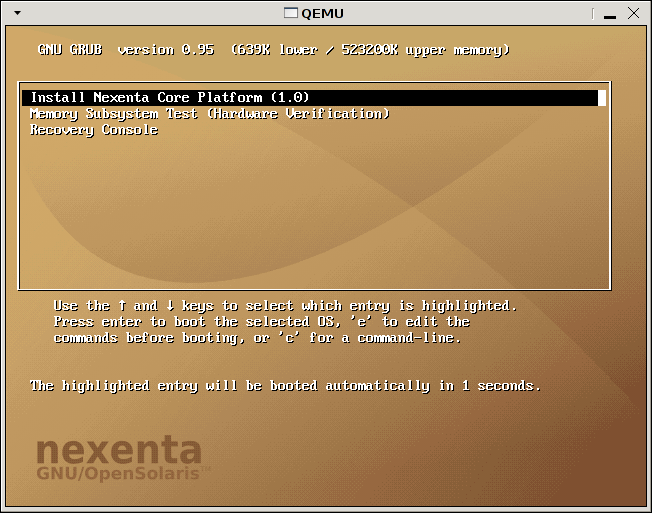
\includegraphics[width=0.5\hsize]{image200804/nexenta1.png}
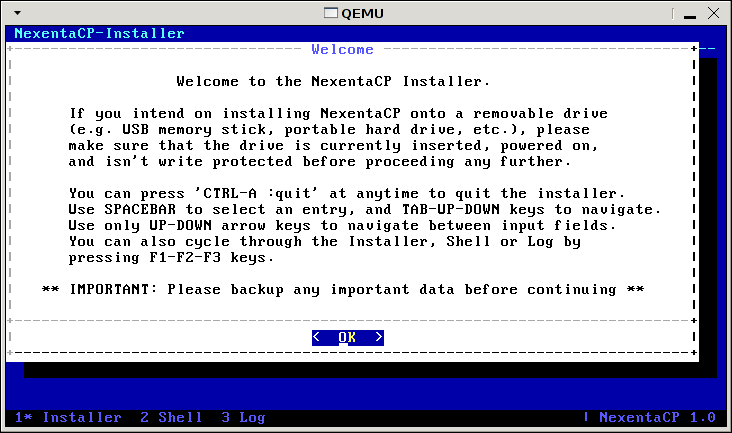
\includegraphics[width=0.5\hsize]{image200804/nexenta2.png}
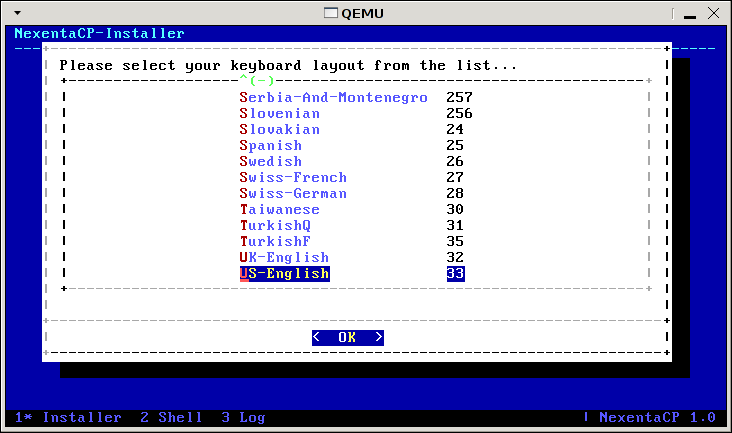
\includegraphics[width=0.5\hsize]{image200804/nexenta3.png}
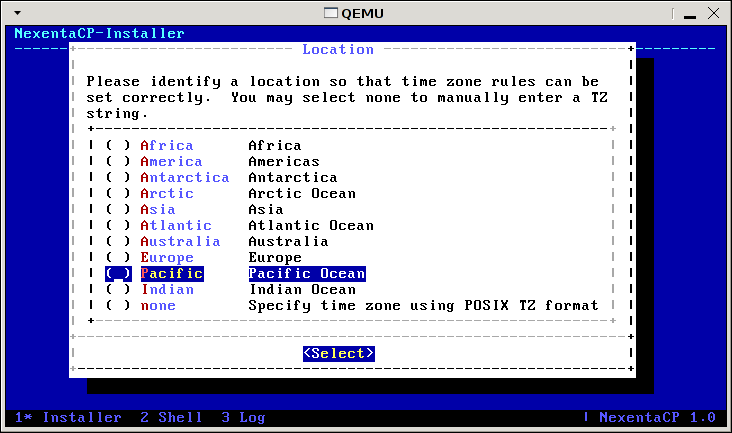
\includegraphics[width=0.5\hsize]{image200804/nexenta4.png}
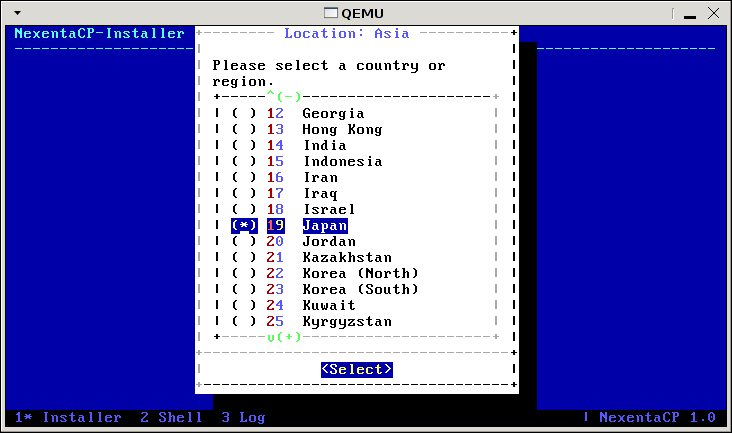
\includegraphics[width=0.5\hsize]{image200804/nexenta5.png}
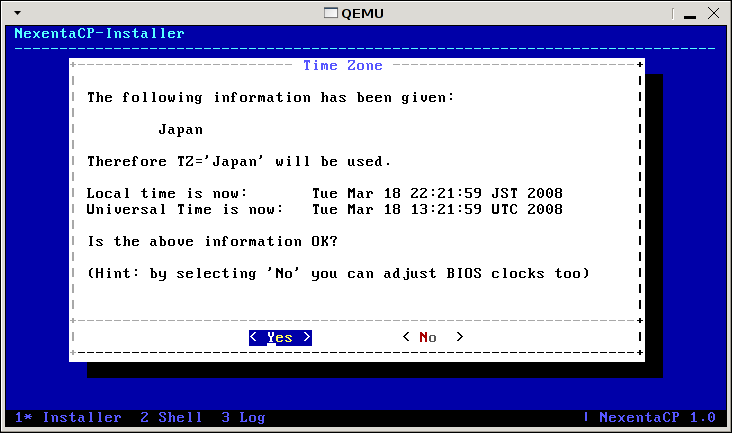
\includegraphics[width=0.5\hsize]{image200804/nexenta6.png}
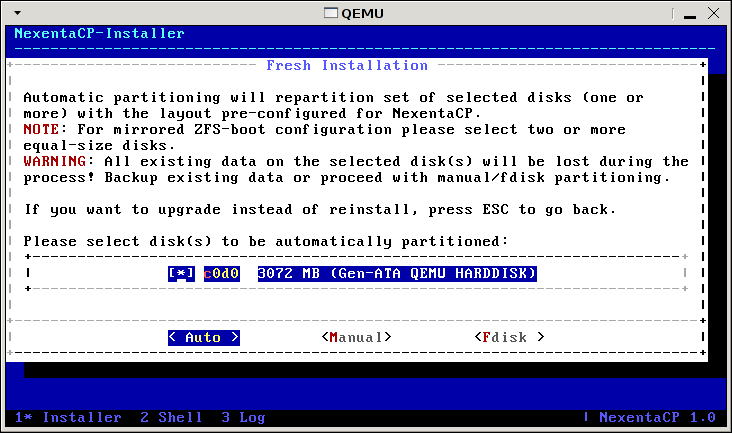
\includegraphics[width=0.5\hsize]{image200804/nexenta7.png}
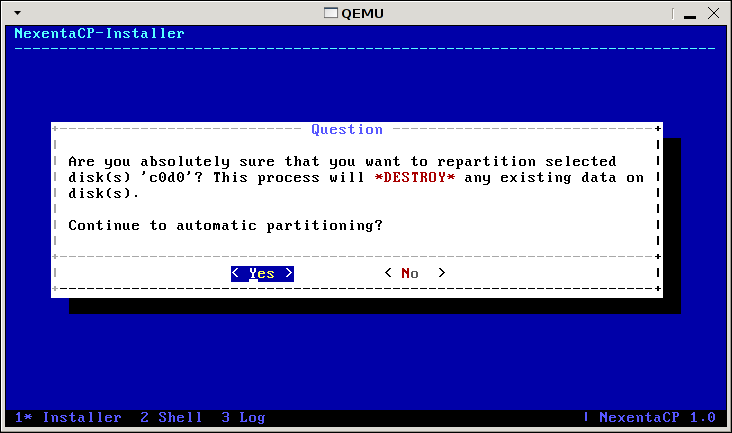
\includegraphics[width=0.5\hsize]{image200804/nexenta8.png}

インストールが開始したらしばし待ちます。\footnote{AMD Athlon 64 3500+ の
マシン(64bit)でkqemuを利用して2時間かかりました}

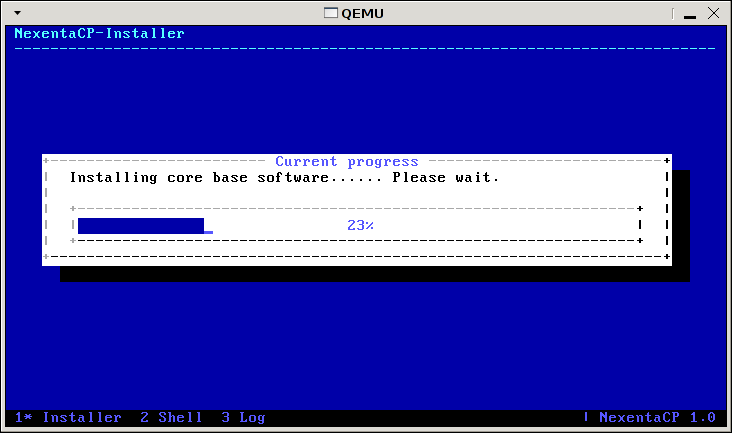
\includegraphics[width=0.5\hsize]{image200804/nexenta9.png}
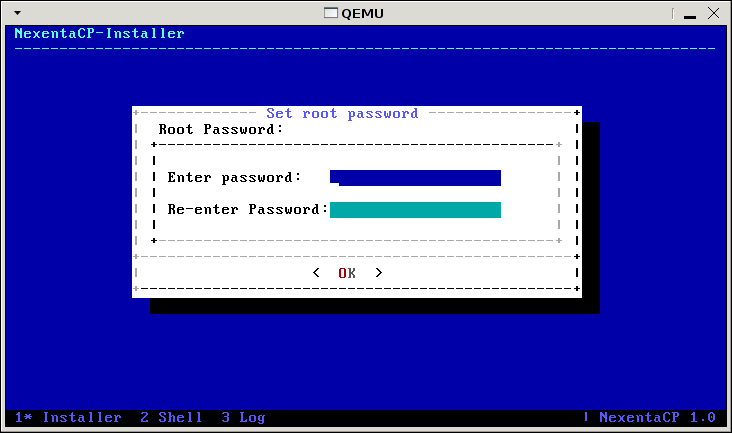
\includegraphics[width=0.5\hsize]{image200804/nexenta10.png}
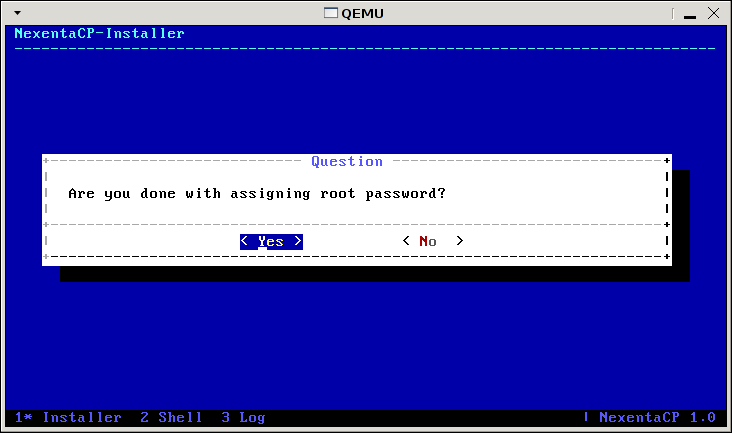
\includegraphics[width=0.5\hsize]{image200804/nexenta11.png}
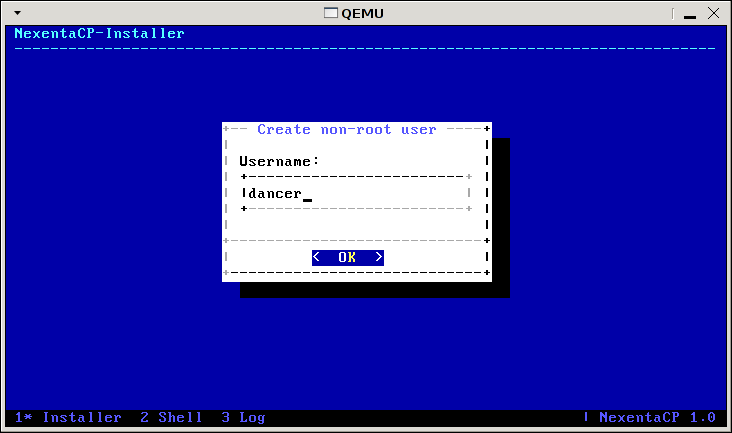
\includegraphics[width=0.5\hsize]{image200804/nexenta12.png}
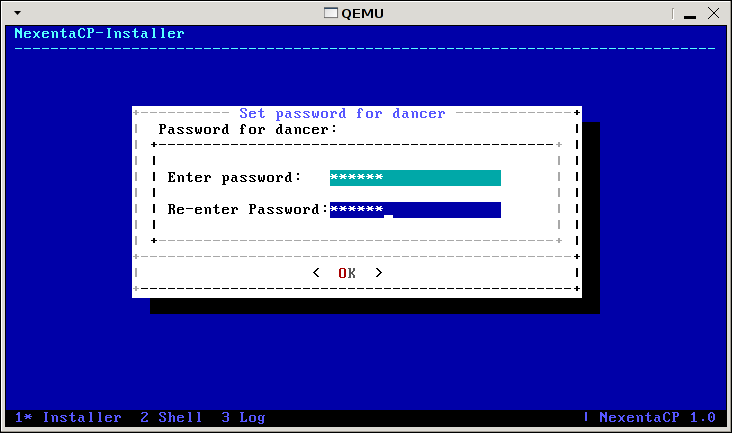
\includegraphics[width=0.5\hsize]{image200804/nexenta13.png}
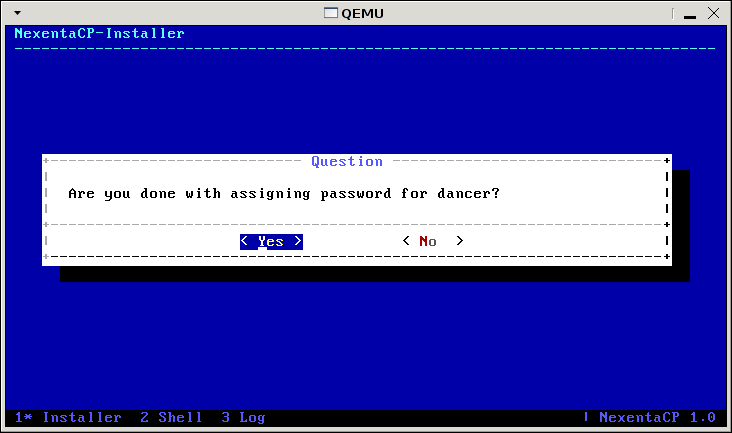
\includegraphics[width=0.5\hsize]{image200804/nexenta14.png}
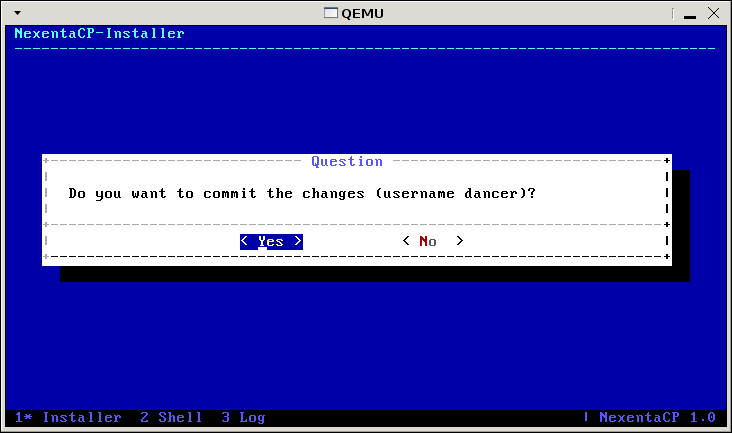
\includegraphics[width=0.5\hsize]{image200804/nexenta15.png}
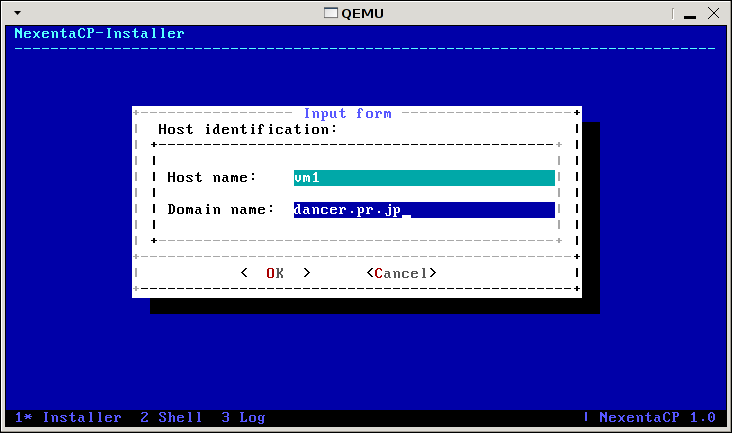
\includegraphics[width=0.5\hsize]{image200804/nexenta16.png}
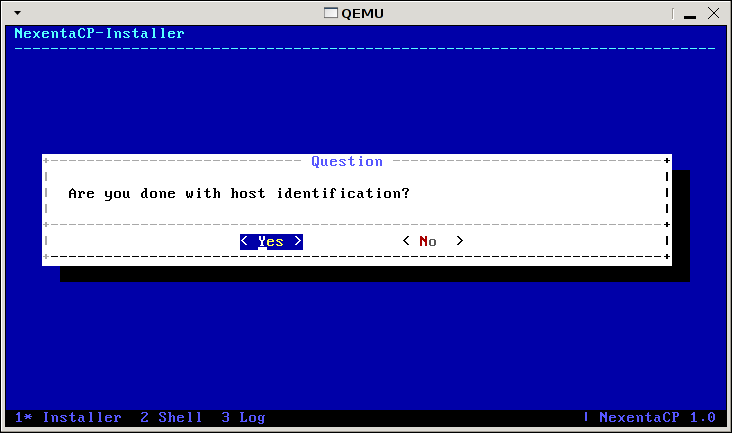
\includegraphics[width=0.5\hsize]{image200804/nexenta17.png}
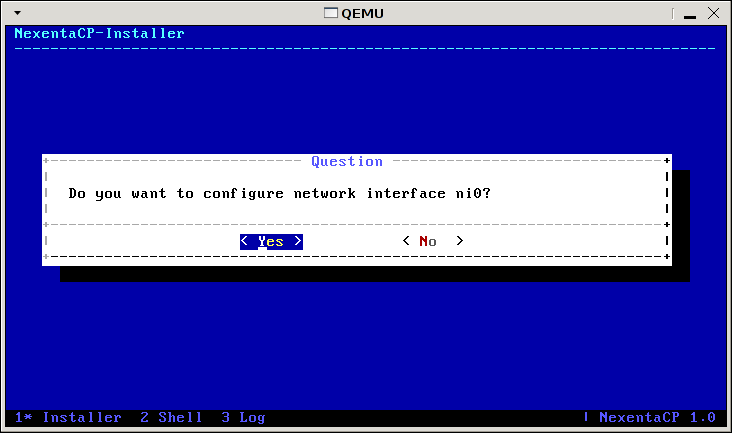
\includegraphics[width=0.5\hsize]{image200804/nexenta18.png}
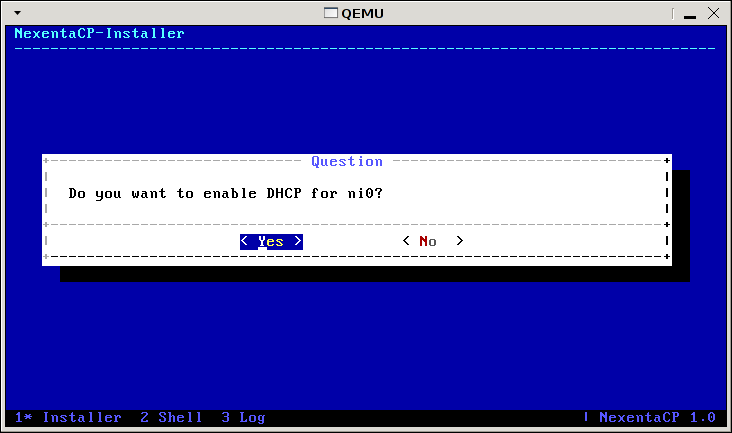
\includegraphics[width=0.5\hsize]{image200804/nexenta19.png}
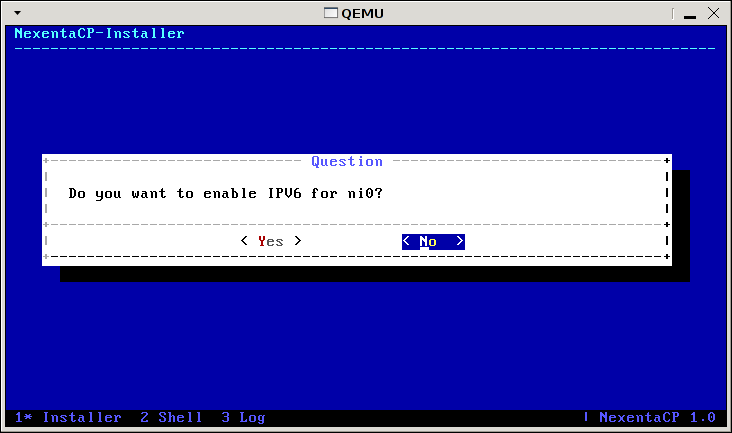
\includegraphics[width=0.5\hsize]{image200804/nexenta20.png}
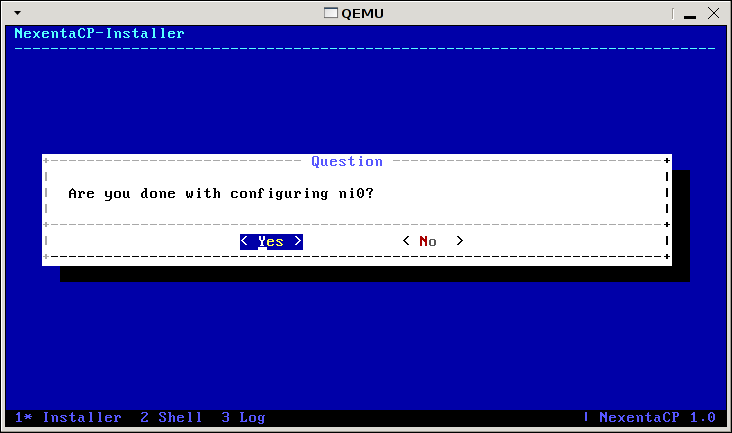
\includegraphics[width=0.5\hsize]{image200804/nexenta21.png}
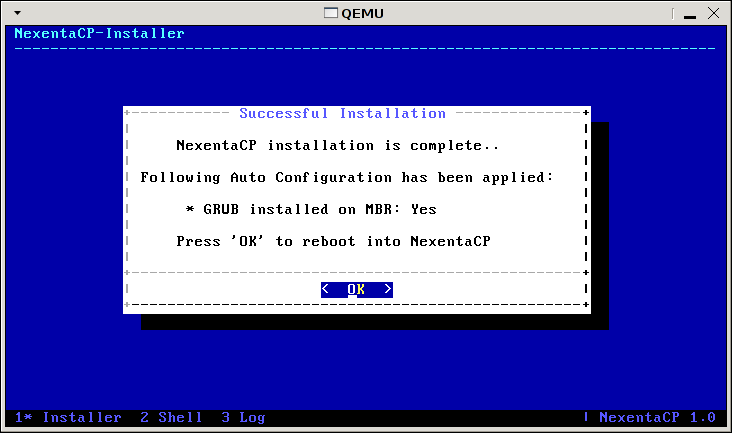
\includegraphics[width=0.5\hsize]{image200804/nexenta22.png}

\subsection{実行してみる}

それでは、インストールしたOSを起動してみましょう。メモリは512MB程度割り
当てないと起動しないようです。

\begin{commandline}
$ qemu-system-x86_64 -hda nexenta.cow \
 -m 512 -kernel-kqemu \
 -redir tcp:2222::22
\end{commandline}

手元のシステムでは、コマンドラインでログインができる状態まで3分程度かかりました。

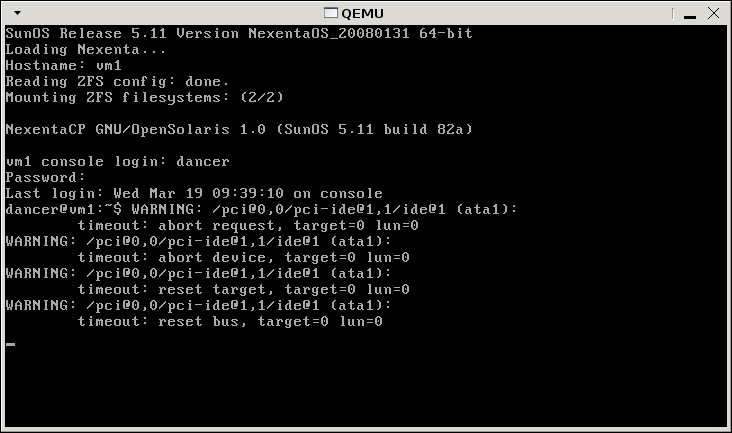
\includegraphics[width=0.5\hsize]{image200804/nexenta23.png}

通常のコンソールのログイン画面が立ち上がり、ログイン可能になります。

デフォルトで sshd \footnote{Debian のパッケージとは異なり、SUNWsshdu,
SUNWsshdr などのパッケージになっています。見た感じは alien で作成されてい
るパッケージのようです。} などもインストールされているようです。
netstat で確認するとlisten しているようですので、ssh でログインして作業
することが可能なようです。
ここでは、 qemu で -redir オプションを使い、 SSHの22番ポートをホストOSの
2222ポートからアクセスできるようにしています。

-nographic -serial stdio オプションも追加してヘッドレスで稼働させることも
可能です。ただし、デフォルトではシリアルコンソールには何も出力されないようです。

ネットワークデバイスは ni0 になっているようです。IPアドレスは qemu の機
能で DHCPで提供されているアドレス(10.0.2.15)になっています。


\subsection{Debian との互換性}

初期インストールのパッケージ数が非常に多いです。OpenSolaris のデフォルト
インストールに相当するものをそのままパッケージにしているのでしょうか?
SUNWではじまるパッケージ名などがそれっぽさを物語ります。

\begin{commandline}
dancer@vm1:~$ dpkg -l | wc -l 
464
dancer@vm1:~$ dpkg -l 
Desired=Unknown/Install/Remove/Purge/Hold
| Status=Not/Installed/Config-files/Unpacked/Failed-config/Half-installed
|/ Err?=(none)/Hold/Reinst-required/X=both-problems (Status,Err: uppercase=bad)
||/ Name           Version        Description
+++-==============-==============-============================================
ii  adduser        3.80nexenta3   Add and remove users and groups
ii  alien          8.73.4         install non-native packages with dpkg
ii  apt            0.6.46.4nexent Advanced front-end for dpkg
ii  apt-utils      0.6.46.4nexent APT utility programs
ii  aptitude       0.4.4-1nexenta terminal-based apt frontend
[中略]
ii  sunw1394       5.11.82-1      Sun IEEE1394 Framework
ii  sunwaac        5.11.82-1      Adaptec AdvanceRaid Controller SCSI HBA Driv
ii  sunwad810      5.11.82-1      SUNW W1100z & W2100z Audio Drivers
ii  sunwadixp      5.11.82-1      SUNW Audio Driver for ATI IXP
ii  sunwadpu320    5.11.82-1      Adaptec Ultra320 Driver
ii  sunwafe        5.11.82-1      ADMtek Ethernet Driver
ii  sunwagp        5.11.82-1      AGP GART Driver
ii  sunwahci       5.11.82-1      Advanced Host Controller Interface (AHCI) SA
ii  sunwamd8111s   5.11.82-1      AMD8111 FAST Ethernet Network Adapter Driver
ii  sunwamr        5.11.82-1      LSI MegaRAID SCSI HBA Driver
[中略]
ii  sunwsshcu      5.11.82-1      SSH Common, (Usr)
ii  sunwsshdr      5.11.82-1      SSH Server, (Root)
ii  sunwsshdu      5.11.82-1      SSH Server, (Usr)
ii  sunwsshr       5.11.82-1      SSH Client and utilities, (Root)
ii  sunwsshu       5.11.82-1      SSH Client and utilities, (Usr)
ii  sunwtavor      5.11.82-1      Sun Tavor HCA driver
[略]
\end{commandline}

\subsection{ないパッケージをビルドしてみた}

/etc/hostsをいじってみようとしたら、シンボリックリンクになってました。し
かも root 権限でも書き込み不可になっています。

\begin{commandline}
root@vm1:/export/home/dancer# ls -l /etc/hosts
lrwxrwxrwx 1 root root 12 Mar 19 08:15 /etc/hosts -> ./inet/hosts
root@vm1:/export/home/dancer# ls -l /etc/inet/hosts -l 
-r--r--r-- 1 root sys 1078 Apr  6 10:28 /etc/inet/hosts
\end{commandline}

気をとりなおして、 /etc/apt/sources.list に適当にソースを追加します。

\begin{commandline}
deb-src http://cdn.debian.or.jp/debian unstable main contrib non-free
\end{commandline}

apt-listbugs が存在しないみたいなので、ビルドしてみようと思います。

まず、なぜだか racc, rdtool が足りないのでビルドしてインストールします。
無事にapt-listbugs 自体もビルドできたので、意気揚々とインストールしてみま
す。

\begin{commandline}
root@vm1:/tmp/apt-listbugs-0.0.88# debi
Selecting previously deselected package apt-listbugs.
(Reading database ... 27441 files and directories currently installed.)
Unpacking apt-listbugs (from apt-listbugs_0.0.88_all.deb) ...
dpkg: dependency problems prevent configuration of apt-listbugs:
 apt-listbugs depends on ruby (>= 1.8); however:
  Package ruby is not installed.
 apt-listbugs depends on libruby1.8 (>= 1.8.5); however:
  Version of libruby1.8 on system is 1.8.4-1nexenta1.3.
 apt-listbugs depends on libdpkg-ruby1.8 (>= 0.3.2); however:
  Package libdpkg-ruby1.8 is not installed.
 apt-listbugs depends on libgettext-ruby1.8; however:
  Package libgettext-ruby1.8 is not installed.
 apt-listbugs depends on libxml-parser-ruby1.8; however:
  Package libxml-parser-ruby1.8 is not installed.
 apt-listbugs depends on libhttp-access2-ruby1.8 (>= 2.0.6); however:
  Package libhttp-access2-ruby1.8 is not installed.
dpkg: error processing apt-listbugs (--install):
 dependency problems - leaving unconfigured
Errors were encountered while processing:
 apt-listbugs
debi: debpkg -i failed
\end{commandline}

残念、いくつかエラーがあるようです。ruby 自体が古いというエラーや、いくつ
かのライブラリが足りないというエラーがでています。

解決できそうな問題も、解決できなさそうな問題もあります。先は長いか?

\subsection{まとめ}

今回はNexenta Core Platformをとりあえず仮想マシンにインストールしてみまし
た。いろいろとDebian GNU/Linuxと違う部分があったので、今後どのように開発
がすすむのか、気になります。


%%%%%%%%%%%%%%%%%
% ここから関西エリア
%%%%%%%%%%%%%%%%%

% 1月


\dancersection{GIS on Debian GNU/Linux!}{清野 陽一}
\index{GIS} 


\subsection{はじめに}
\subsubsection{社会的整備の進展}

\begin{itemize}
 \item 国際情勢
       \begin{itemize}
	\item 地図情報を電子化して扱おうという試みは1960年代ごろから始まってい
	      ます。当初は研究目的でした。
	\item メインフレーム上ではなく、ワークステーションやパーソナルコンピュー
	      タの発達に伴い、1980年代頃からこれらのコンピュータ上で動かせるシ
	      ステムが普及し始めました。
	\item 後述する地上観測衛星(ランドサット衛星1号機の打ち上げは1972年)や
	      スペースシャトルの運用により、リモートセンシングなどの活用が1970
	      年代より行われるようになりました。
       \end{itemize}
 \item 日本国内
 \begin{itemize}
  \item 行政サイド \\
	日本においては、国土に関する数値情報の電子化
	\begin{quotation}
	 「平成7年1月の阪神・
	 淡路大震災の反省等をきっかけに、政府において、GISに関する本格的な
	 取組が始まった。」(国土地理院
	 GIS\footnote{\url{http://www.gsi.go.jp/GIS/whatisgis.html}}による) 
	\end{quotation}
	→国を挙げての政策実施。2002年の小泉内閣における「e-Japan重点計
	画-2002」の重点政策のうち、4番目の「行政の情報化及び公共分野にお
	ける情報通信技術の活用の推進」においてGISの推進が盛り込まれる。
	ex)国土地理院の数値地図(CD-ROM版)は平成9(1997)年頃から整備される
	ようになってきています。
  \item 建設サイド
	\begin{itemize}
	 \item CAD(Computer Aided Design)の普及
	 \item 電子納品・標準化
	 \item 建設省・国土交通省の後押し
	\end{itemize}
 \end{itemize}
\end{itemize}

\subsubsection{個人レベル}
\begin{itemize}
 \item Google Earth、NASA World Windなどの無料かつ高性能なデスクトップ地
       図ビューワーの登場 \\
       →"Google Earthショック"
 \item Google MapなどのWebマッピングサイト \\
       →MashUpが流行\\
       →空間情報を個人が扱う時代になった
\end{itemize}

\subsection{GISとは}
\subsubsection{定義}
\begin{itemize}
 \item 国土地理院\footnote{\url{http://www.gsi.go.jp/GIS/whatisgis.html}}の説明
       \begin{quotation}
	地理情報システム(GIS:Geographic Information System)は、地理的位置を手がかりに、位置に関する
	情報を持ったデータ(空間データ)を総合的に管理・加工し、視覚的に表示し、高度な分析や迅速な判断
	を可能にする技術です。 
       \end{quotation}
 \item GISポータルサイト
       \footnote{\url{http://www.gis.go.jp/contents/about/whatis/index.html}}の説
       明
       \begin{quotation}
	GIS(Geographic Information System:地理情報システム)とは、位置や空間に関する様々な情報を、コ
	ンピュータを用いて重ね合わせ、情報の分析・解析をおこなったり、情報を視覚的に表示させるシステム
	です。元々は専門的な分野での利用が一般的でしたが、最近では、私たちの生活の中での身近な利用へと
	、その活用範囲が広がってきています。 
       \end{quotation}
 \item 国土交通省国土計画局
       \footnote{\url{http://www.mlit.go.jp/kokudokeikaku/gis/aboutgis/index.html}}
       の説明
       \begin{quotation}
	位置や空間に関する情報をもったデータ(空間データ)を総合的に管理・加工し、視覚的に表示できる高
	度な分析や迅速な判断を可能にする技術です。 
       \end{quotation}
 \item ESRIジャパン社
       \footnote{\url{http://www.esrij.com/whatisgis/gis/index.shtml}}の説明
       \begin{quotation}
	GISとは、Geographic Information Systemの略で、広義には「実世界を空間的に管理することにより
	、より合理的な意思決定を行おうとするアプローチ全般」を意味しますが、狭義には、「空間情報を作成
	、加工、管理、分析、表現、共有するための情報テクノロジ」を意味します。 
       \end{quotation}
 \item インフォマティクス社
       \footnote{\url{http://www.informatix.co.jp/sis/aboutgis/aboutgis.html}}の
       説明
       \begin{quotation}
	GISとは、Geographical Information Systems(地理情報システム)の略で地図上に様々な情報を重ね
	合わせて表示・編集したり、分析するシステムのことをいいます。
       \end{quotation}
\end{itemize}

\begin{itembox}[c]{"GIS"と"GPS"の違いってわかる?}
混同している人を良く見かけます。GPS とは "Global Positioning System"の略です。

全地球測位システム、汎地球測位システムの事です。アメリカの衛星システムや元軍事用として使われています。

カーナビとか携帯電話に入っているものです。
\end{itembox}

\subsubsection{大別して2タイプ}
\begin{itemize}
 \item 管理系GIS
       \begin{itemize}
	\item 統合型・全庁型 \\
	      商用製品が主流。ラージスケール指向。分析もできます。\\
	      →ESRI社ArcGIS、インフォマティクス社のSIS、MapInfo社のMapInfoなどです。
	      \\
	      →実際、助成金などでお金がある人は、個人研究者でも導入する人は多
	      いようです。\\
	      →その場合、操作方法を知っていることで就職時のアドバンテージにもなるようです。
	\item 表示系:Google Earth、Google Mapみたいなものです。
	\begin{itemize}
	 \item mapserver:WebGISサーバ
	       \footnote{\url{http://mapserver.gis.umn.edu/}}
	 \item ka-Map\footnote{\url{http://ka-map.maptools.org/}}
	\end{itemize}
	\item CADとの関係\\
	      設計・測量・建設・土木・防災と密接に連携します。\\
	      →境目が曖昧になってきています\\
	      →Autodesk(AutoCAD)社のオープンソースへの参入
       \end{itemize}
 \item 解析系GIS
       \begin{itemize}
	\item GRASS GIS\footnote{\url{http://grass.itc.it/}}\\
	      1980年代半ばから開発開始しました。
	\item Quantum GIS\footnote{\url{http://www.qgis.org/}}\\
	      高機能なビューワ。簡単な解析機能も持ちます。
	\item SAGA
	      GIS\footnote{\url{http://www.saga-gis.uni-goettingen.de/html/index.php}}\\
	      Release 2.0.1はGentoo LinuxのPortage用が用意されてるようです。
	\item Mandara\footnote{\url{http://www5c.biglobe.ne.jp/~mandara/}}\\
	      Windows用のGISソフトです。初心者向けです。GISがどういうものかをてっとり早
	      く知りたい人にはお手軽かもしれません。MS Excelとの連携もできます。
       \end{itemize}
\end{itemize}

\subsection{最近の話題}
\begin{itemize}
 \item OSGeo財団\footnote{\url{http://www.osgeo.org/node/271}}日本支部\footnote{\url{http://www.osgeo.jp/}}\\
       大阪市立大学や株式会社オークニーなどが中心
 \item 関西オープンソース2007におけるカンファレンス\footnote{\url{http://www.osgeo.jp/?page_id=8}}\\
       「特別企画:OSGeo.JP 創造都市を支えるオープンソース GISの最前線」
 \item 書籍の整備
       \begin{itemize}
	\item 『入門Webマッピング(\textit{Web Mapping Illustrated})』(2006年5月、
	      オライリー)\footnote{\url{http://www.oreilly.co.jp/books/4873112826/}}
	\item \textit{Open Source Gis: A Grass Gis Approach}(2007年末に3rd
	      Editionが出た、Springer)\footnote{\url{http://www.grassbook.org/}}
       \end{itemize}
\end{itemize}

\subsection{なぜDebian GNU/Linuxか?}
\subsubsection{Debian GNU/Linuxを選んだ動機(個人的経験)}
\begin{itemize}
 \item[★] オープンソースなソフトウェアが使いたかった。\\
       →高機能なプロプライエタリなソフトウェアは沢山あるが、高価!組織や補助金で導入した場合
	   はライセンスの問題が$\dots$。\\
	→プログラマブルなのもいいかも(勉強になるかも)
 \item[★] DebianGISのようなプロジェクトがある(最近は停滞気味?)
 \item[○] 初心者的に、パッケージの管理が楽そうだった(APT万歳!!)。
 \item[●] でも、使いこなせるなら他のディストリビューションでもOK?\\
	   →ソースコードは公開されてることが多いし、Debian GNU/Linuxじゃ
	   なきゃダメなバイナリというのは無いと思う。\\
	   →Windows上で使える環境も着々と進んできている。まだUnix/Linux
	   にアドバンテージがありますが。\\
	   →MacOSはGISはあんまり得意じゃないかも$\dots$。
 \item[●] 海外ではMandrivaとか(かつてのArcheOSとか)Gentoo
	   Linux(Gentoo-GIS overlay Project \footnote{\url{http://gentoo-gis.sourceforge.net/}}なんての
	   がある。)などもよく利用されているようです。
 \item[●] 最近は人に勧めるとしたらUbuntuか$\dots$。(個人的に紹介実績有り)
\end{itemize}

\subsubsection{Debian GNU/Linuxにおけるパッケージ、ライブラリなど}

DebianGIS\footnote{\url{http://wiki.debian.org/DebianGis}}に紹介されている
Debian GNU/Linuxにおけるパッケージ、ライブラリを以下に示します。
\begin{commandline}
Geospatial packages of core concern
    Meta-packages
        *education-geography task from debian-edu: DebianGIS recommends these additions: qgis, gmt, gdal, proj.
 (education-geography already depends on grass):
    Binary packages
        *PostGIS
            RDBMSのPostgreSQLの地理情報拡張
        *GDAL(Geospatial Data Abstraction Library 地理空間データ抽象化ライブラリ?)
            座標系(投影)変換ライブラリ
        *GRASS
        *QuantumGIS. Includes qgis-plugin-grass
        *Mapserver
        *GEOS
        *PROJ: proj-doc: there are PDF files available, perhaps those would be better?
        *Earth3D
        *gpsd
        *gpsdrive
        *gpx2shp
        *gpsman
        *gpsmanshp
        *gpstrans
        *gpsbabel
        *thuban
        *gmt
        *OpenSceneGraph
        *OpenThreads
        *Avce00 and E00compr
        *OGDI
        *OpenJUMP: in debian/contrib, because it depend on batik and sun jre. Work is being done to get batik into 
debian/main, and openjump to work with GNU Classpath. Packaged instead of JUMP
        *JTS
        *TerraLib
        *mapnik
        *marble
        *Viking: a GPS track editor and analyzer
        Useful packages to be packaged
        Sorted by approximate priority.
            Libraries and bindings
            *Python Shapelib binding
            *Python Cartographic Library (PCL)
            *Tcl Shapelib binding
            *Ruby Shapelib binding
        Desktop/Analysis/Database
            *Ossim: currently being worked on (Francesco Lovergine)
            *PostLBS: powerful routing solution for PostgreSQL/PostGIS
            *TerraView: powerful GIS based on TerraLib (already in Debian, but obsolete)
            *OpenModeller: species occurrence modelling software
            *r-spatial: R/GRASS interface for GRASS 6 and other spatial software for R
                R言語:統計処理。空間統計ライブラリ
            *garmin-utils: similar in scope and function to gpstrans, but works with modern serial Garmins. 
See also the NetBSD port
            *e-foto: aerial photogrammetry. See this unanswered post
        Data
        OpenStreetMap
            *OpenStreetmap: Useful for upcoming release of gpsdrive
            *josm: Java Open Street Map Editor
            *gosmore: viewer of OSM XML data such as the planet.osm
        Sample datasets
            * GRASS's Spearfish dataset
            * OSGeo's NC sample dataset
\end{commandline}
\begin{commandline}
    Java
        *gvSIG (top priority)
        *uDig: User-friendly Desktop Internet GIS
        *GeoServer
        *Postgisdriver-JUMP: currently being worked on. Contrib - depends on jump
        *GeoTools: Java GIS Toolkit
        *Deegree2 and iGeoPortal: currently being worked on. Binary package structure not yet clear.
        *NASA World Wind (Java version): Needs JOGL and perhaps SUN Java
        *JOGL: Java
        *Kosmos Desktop GIS derived from OpenJUMP (an unofficial package available)
            For more info on the Java state in Debian, see the moving java to Debian/main page.
    Live Web Apps
        *PyWPS: Python Web Processing Service
        *OpenLayers, TileCache, FeatureServer (all from MetaCarta)
        *p.mapper (unofficial packages available
    3D Visualization
        *ParaView: Very useful for 3D rapresentation of GRASS rasters and vectors
        *Visual Terrain Project: proposed
        *VisIt: 3D visualization
        *X3D: modern version of VRML, various libs & apps
        *OpenDX: the open source version of IBM's Visualization Data Explorer. Uses the IBM Public License
        *MINI: proposed, needed for VTerrain
        *OpenProducer: proposed, useful for OpenSceneGraph
    Lower Priority
        *Shape file utilities, including ShapeChecker
        *http://www.primagis.fi/ map extension for Plone; it builds on top of Mapserver, 
Python Cartographic Library (PCL) and Cartographic Objects for Zope (ZCO)
        *OpenEV: currently being worked on (Alex Bodnaru); old version, based on gtk1; the new one, based on 
gtk2, is still unsuitable to packaging
        *MB-System: multibeam, interferometry, and sidescan sonar data processing (GPL)
        *PhpPgGIS: ITP #381974. Project apparently inactive
        *Open3D GIS: Requires FreeWRL, see http://sourceforge.net/projects/freewrl/.
 Project apparently dead? https://sourceforge.net/projects/open3dgis/
        *dxf2svg: also the reciprocal svg2dxf (depends on pstoedit)
        *JGrass: currently being worked on. Contrib - needs jdk1.4, several contrib packages. Currently being
 fused with uDig - better postpone packaging until settled down
\end{commandline}

この他にFOSS4G Toolkit CDやArcheOS(Mandrivaだったが最近Ubuntu化した)など
のLive CDもあります。
\footnote{FOSS4G Toolkit CDはMandriva向けのRPMセットとして配布するのみとなったようです。}

\subsection{空間データ}

以前は必要とする者が自ら取得することが一般的であったが、最近では各種空間
データが整備されてきている。

\subsubsection{国内}
\begin{itemize}
 \item 国土地理院発行の各種数値地図(有償)\footnote{\url{http://www.gsi.go.jp/}}\\
       ただし、近年、情報公開により閲覧を目的としてデータの無償公開が進
       んでいる。\\
       ex)国土地理院数値地図(空間データ基盤)の閲覧(試験公開)
       \footnote{\url{http://sdf.gsi.go.jp/}}
 \item 電子国土ポータル\footnote{\url{http://portal.cyberjapan.jp/index.html}}\\
       各種地図の閲覧を主眼。精細なベクトルデータを提供。専用プラグイン
       を用いて各自がWeb地図作成を行える。
 \item 陸域観測技術衛星「だいち」(ALOS)\\
       宇宙航空研究開発機構(JAXA\footnote{\url{http://www.jaxa.jp/index_j.html}})
       が2006年1月24日に打ち上げた衛星の観測データ。有料?
\end{itemize}

「高精度で標高抽出を行うためのパンクロマチック立体視センサ(PRISM)、およ
び土地被覆の観測を高精度に行うための高性能可視近赤外放射計2型(AVNIR-2)、
昼夜の別なく、また天候によらず陸域の観測が可能なフェーズドアレイ方式Lバ
ンド合成開口レーダ(PALSAR)の3つの地球観測センサを搭載」

※2008年1月8日、予定した精度が取得できないのではないかとの報道
\footnote{\url{http://www.asahi.com/special/space/TKY200801090162.html}}
がなされたが、その後の調査により、同年同月16日、新たな方法を用いることで懸念されていた
問題は改善できるとの発表がなされた
\footnote{\url{http://www.jaxa.jp/press/2008/01/20080116_sac_daichi_j.html}}。

\subsubsection{地球規模}
\begin{itemize}
 \item スペースシャトル地形データ Shuttle Radar Topography Mission
       (SRTM)\\
       1994年より実験開始。現在主に利用されているのは2000年に行われた第3回実験
       によって取得されたデータ。11日間の飛行で両極を除く地上の陸地の約
       80%、全人口密集地の約95%をカバーするデータを取得した。

       NASAのFTPサイト\footnote{\url{ftp://e0srp01u.ecs.nasa.gov/srtm/}}よりデータをダ
       ウンロード可能。一部有料。

       DEM(Digital Elevation Model)の作成用
 \item ランドサット衛星画像 Landsat Imagery (TM,
       ETM+)\footnote{\url{http://www.eorc.jaxa.jp/hatoyama/satellite/satdata/landsat_j.html}}\\
       メリーランド大学
       \footnote{\url{http://glcfapp.umiacs.umd.edu:8080/esdi/index.jsp}}
       からデータをダウンロード可能。
       様々な波長の光の反射データ。リモートセンシング用。
 \item 商用衛星画像データ\\
       Google EarthやGoogle Mapなどでは高精細な商用衛星画像データが用い
       られている。Earthsat社やDigital Globe社、Bluesky社など。\\
       確かに解像度が高く利用価値は高いが、非常に高価なので、費用対効果を考えて利用されている。
\end{itemize}

でも結局研究目的の場合などは、今でも自分達でデータを取得しなければならないことの方が多いです。
なので、いかに効率的に、必要とされ、正確・詳細な空間データを取得するかが問題となります。

\subsection{おわりに}
\subsubsection{まとめ}
以前に比べて環境は格段に良くなっています。
特に、こちらから能動的に各種データの整備を要求・もしくは自ら多大なコスト
をかけて取得しなくても、次々と空間基盤データの整備が行われてきています。
表示系の地図サイトなどは個人レベルで管理・運用できる環境が整っています。\\
皆さんもちょっと触ってみませんか?

\subsubsection{反省点}
今回はGISの概要を説明することで大半を消費してしまいました。より具体的な話が
出来なかったのが悔やまれます。
しかし、実際に使ってみないと実感が湧かないのも事実です。
また、具体的な課題がないと、なかなか触るきっかけもないかもしれません。

\dancersection{DebianでPCクラスタを作ってみよう}{中尾 昌広}
\index{PC Cluster}

\subsection{はじめに}
安価で高速な並列計算機システムであるPCクラスタを、Debianを使ってセットアッ
プする方法について説明します。

\subsubsection{PCクラスタとは何か?}
クラスタ(cluster) とは英語で「ブドウの房、同じものが群らがっている様」みたいな意味です。
つまり、PCクラスタとは、複数台のPCをブドウのように(LANケーブルで)相互接続し、
それらを協調動作させるシステムのことです。

\begin{figure}[!htbp]
 \begin{center}
 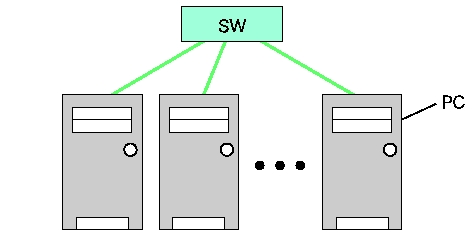
\includegraphics[width=82mm]{image200802/cluster.png}
  \caption{クラスタの概念図}
  \label{fig:cluster}
 \end{center}
\end{figure}
\vspace{-3mm}

\subsubsection{PCクラスタをつくる理由}
高速な計算機環境が欲しいけど、スーパーコンピュータみたいな高価な専用並列計算機はとても買えません。
そこで、普通の電気屋で売っているようなPC をクラスタ化して、安価に並列計算環境を作ろう、ということが考えられました。

PCクラスタには大きく分けて、HA(High Availability)クラスタとHPC(High Performance Computing)クラスタがあります。
HAクラスタとは、高可用性を持つシステム、つまりサービスを止まりにくくすることを目的としたクラスタシステムです。
最近はWeb系のサーバでこのシステムがよく利用されています。
HPCクラスタとは、科学計算分野などでおいて、ものすごく時間のかかる処理を、複数台のPCに分散させて、
高速に結果を得ることを目的としたクラスタシステムです。
企業のメーカでも、車体や航空機を設計する際のシミュレーションなどに用いられています。

本資料とプレゼンでは基本的にHPCクラスタについての話ですが、HAクラスタに共通している点も多いはずです。

\subsubsection{DebianでPCクラスタを作る理由}
\begin{itemize}
\item Debianには数多くのPCクラスタ用ツールがある。
\item PCクラスタのOSとして普通のDebianを利用するので、PCクラスタツール以外の有用なツールも数多く利用できる。
\item コミュニティが活発(debian-usersで質問に答えてくれる人達は素晴らしい)。
\item aptが楽。
\end{itemize}

\subsection{PCクラスタの作り方}
並列計算ができるまでを目標として、PCクラスタシステムをセットアップする手順を説明します。
\begin{enumerate}
\item PCクラスタを構成する部品(PC、LANケーブル、スイッチングハブ)を用意し、それぞれ接続する。
\item 用意したPCにDebian GNU/Linuxをインストールする。
\item 自分が必要とするコンパイラと並列計算ライブラリをインストールする。
      並列計算ライブラリはmpichとPVMがよく用いられる。
      今回はmpichを使う。
\begin{commandline}
 # aptitude install mpich-bin libmpich1.0-dev gcc g77 g++
\end{commandline}
      インストール後に並列計算に用いるホスト名(もしくはIPアドレス)を
      /etc/mpich/machines.LINUX記述する。
\item クラスタ内ネットワークでは、速度重視のため暗号化なしで通信を行いた
      いので、rsh-serverとrsh-clientをインストールする。
\begin{commandline}
 # aptitude install rsh-server rsh-client
\end{commandline}
      インストール後にrshを許可するホスト名(もしくはIPアドレス)を
      /etc/hosts.equivに記述する。
\item NFSを使って/home以下の共有を行うと便利なため、PCクラスタを構成する
      PCの1台にnfs-kernel-serverをインストールする。
\begin{commandline}
 # aptitude install nfs-kernel-server
\end{commandline}
      そして、nfs-kernel-serverをインストールしたPCの/etc/exportsに、ど
      のPCにNFSのサービスを許可するかの情報を記述する。
\begin{commandline}
 【/etc/exportsの例】
 /home   192.168.1.0/255.255.255.0(rw,async,no_subtree_check)
\end{commandline}
      /etc/exports の変更後にNFSのサービスを再起動させる。
\begin{commandline}
 # /etc/init.d/nfs-kernel-server restart
\end{commandline}
      そして、nfs-kernel-serverをインストールしたPC以外は、mountコマンド
      を用いてNFSサーバにマウントする。
\begin{commandline}
 # mount -t nfs (NFSサーバ):/home /home
\end{commandline}
      以上で、PCクラスタの完成です。簡単です。
      意外かもしれませんが、並列計算ライブラリ以外は特殊なソフトウェアを用いていません。
      このように既存のソフトウェアを有効活用できる所が、PCクラスタの大きな特徴です。
 \item 並列計算用サンプルファイルが、
       /usr/share/doc/libmpich1.0-dev/examples/cpi.cにあるので、実行して
       みましょう。
\begin{commandline}
 $ mpicc cpi.c -o pi 【コンパイル】
 $ mpirun -np 5 pi   【実行】
\end{commandline}
       cpi.cは$\pi$の値を計算するプログラムです。
       mpiccというコマンドでC言語で書かれた並列計算プログラムをコンパイルします。
       Fortranの場合はmpif77、C++の場合はmpicxxなどを用います。

       そして、mpirunというコマンドで、並列計算プログラムを実行します。
       引数の-np以降はプロセス数を指定しています。
       また、並列計算に使用したいマシンを指定する際は、-machinefileというオプションを利用します。

\begin{commandline}
 $ mpirun -np 5 -machinefile hoge.txt pi
\end{commandline}

       この場合、hoge.txtに並列計算に使用したいホスト名を書くと、そのPC
       で並列計算されます。
\end{enumerate}

\subsection{クラスタで使うと便利なソフトウェア}
Gangliaという各ノードの負荷、生死をWebブラウザから確認できるソフトウェアです。
日、週、月、年といった単位でクラスタ全体のロードアベレージの傾向も見ることができます。

\begin{figure}[htbp]
 \begin{center}
  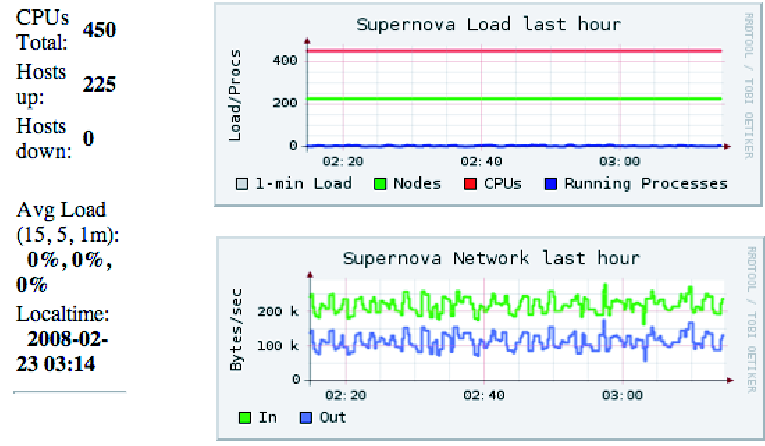
\includegraphics[width=100mm]{image200802/ganglia.png}
  \caption{Ganglia}
  \label{fig:ganglia}
 \end{center}
\end{figure}

\subsection{おわりに}
駆け足でクラスタの概要とセットアップ手順について説明しました。
Debianでクラスタを作るのは簡単だというのが伝われば幸いです。

\subsection{参考文献}
\begin{itemize}
\item 同志社大学知的システムデザイン研究室(\url{http://mikilab.doshisha.ac.jp/})
\item 超並列計算研究会(\url{http://www.is.doshisha.ac.jp/SMPP/})
\end{itemize}


\dancersection{資料作成基礎(TeX)}{山下 尊也}
\index{latex@\LaTeX}
\index{tex}

\subsection{インストール}
今回、対象とするものは2008年2月21日現在のstableであるetchを対象とします。
私のセッションでは最小限の事しか述べないため、YaTeXなどを活用したい方は、
関連URLや東京エリア Debian 勉強会2007年12月の資料\footnote{whizzytexなど
を用いてプレビューさせるなど色々と技が載っています。}をご覧下さい。

\subsubsection{/etc/apt/sources.listの確認}

non-free に含まれているものも利用するため、/etc/apt/sources.listは以下のようにしておい
て下さい。

\begin{commandline}
deb http://ftp.debian.or.jp/debian/ etch main contrib non-free
\end{commandline}

\subsubsection{teTeX と pTeX一式のインストール}
\begin{commandline}
 $ sudo aptitude install ptex-bin
\end{commandline}

\subsubsection{奥村さんの新クラスファイルのインストール}
\begin{commandline}
 $ sudo aptitude install okumura-clsfiles
\end{commandline}

\subsubsection{dvipdfmxのインストール}
\begin{commandline}
 $ sudo aptitude install dvipdfmx
\end{commandline}

\subsubsection{Adobe ReaderおよびCMAPのインストール}
EtchのEvinceには日本語のフォントを埋め込んでない場合に文字が化けると言うバグ 
\footnote{いくやさんが修正したものを配布しています。
\url{http://ikuya.info/wiki/index.php?etchpackages} 
ただ、2008年2月22日現在のunstableでも、Evinceには、popplerの問題があり、
 \url{http://lists.debian.or.jp/debian-devel/200712/msg00000.html}これは、
AdobeとのCMAP問題に繋がるので、
Adobe Readerで見る事をお勧めします。
}
があるので、PDFを見るためにAdobe Readerをインストールします。

Adobe Readerの配布ページ
\footnote{\url{http://www.adobe.com/jp/products/acrobat/readstep2.html}}
にアクセスし、Adobe Readerのdebパッケージを取ってきます。

\begin{commandline}
 $ sudo dpkg -i AdobeReader_jpn-8.1.2-1.i386.deb
 $ sudo aptitude install cmap-adobe-japan1 cmap-adobe-japan2
\end{commandline}

\subsubsection{YaTeX(野鳥)のインストール}

エディタとしてEmacsを使っている人は、YaTeXと呼ばれる
\LaTeX 入力支援環境があるので、それを利用すれば良いでしょう。
\footnote{Emacsを使っていない方でも、VIM-\LaTeX
(\url{http://vim-latex.sourceforge.net/})や
KDE環境にKile(\url{http://kile.sourceforge.net/})という
\LaTeX を編集する環境があるようです。
}

\begin{commandline}
 $ sudo aptitude install yatex emacs21
\end{commandline}

文字コードは iso-2022-jp で統一しています\footnote{Windows 版と Linux 版
の ptex で共通して扱える文字コードにしたという経緯があります。ただし現状
Windows で全部できる状況ではありません。}。たとえば、emacs + yatex を使用
している場合で iso-2022-jp をデフォルトにするには、下記のような設定を
\texttt{.emacs} にかけばよいでしょう。

\begin{commandline}
(add-hook 'yatex-mode-hook
	  '(lambda () 
	     (progn 
	       (if (string-match "^/home/user/monthly-report/" default-directory)
		   (progn (set-buffer-file-coding-system 'iso-2022-jp)
			  (set-buffer-modified-p nil))))))
\end{commandline}

\texttt{.emacs}の例です。

\begin{commandline}
(setq auto-mode-alist
      (cons (cons "\\.tex$" 'yatex-mode) auto-mode-alist))
(autoload 'yatex-mode "yatex" "Yet Another LaTeX mode" t)
(defvar YaTeX-dvi2-command-ext-alist
  '(("xdvi" . ".dvi")
    ("ghostview\\|gv" . ".ps")
    ("acroread" . ".pdf")))
 (setq dvi2-command "acroread")
(setq dviprint-command-format "dvipdfmx `basename %s pdf`dvi")
;;; 色付け
(setq YaTeX-use-font-lock t)
(add-hook 'yatex-mode-hook
	  '(lambda () 
	     (progn 
	       (if (string-match "^/home/user/monthly-report/" default-directory)
		   (progn (set-buffer-file-coding-system 'iso-2022-jp)
			  (set-buffer-modified-p nil))))))
\end{commandline}

\subsection{文章の編集}

\LaTeX は最初は難しいと感じるかもしれませんが、基本は HTML と似たような
ものなので、まずはソースを読む事から始めてみると良いかもしれません。
\LaTeX についてさらに知りたい方は、
「[改訂第4版] \LaTeX 2美文書作成入門
(大型本) 奥村 晴彦 (著) 」
などの本を読む事をお勧めします。

\subsubsection{リポジトリからデータを取ってくる}
現在、関西 Debian 勉強会では、リポジトリの用意が出来ていないため、
東京エリア Debian 勉強会のリポジトリを借りている状態です。

\begin{commandline}
 $ sudo aptitude install git-core
 $ git clone git://git.debian.org/git/tokyodebian/monthly-report.git
\end{commandline}

ドキュメントは p\LaTeX{}で作成しています。ファイル名として下記になってい
ます。(YYYY)(MM)は、年と月で、例えば2008年02月であれば 200802 です。

\begin{itemize}
 \item debianmeetingresume(YYYY)(MM)-kansai.tex

事前配布資料
 \item debianmeetingresume(YYYY)(MM)-kansai-presentation.tex

プレゼンテーション用 (prosperを利用)
 \item image(YYYY)(MM)

画像ファイルなどの置き場
\end{itemize}

\subsubsection{基本部分の説明}

スタイルファイルは kansaimonthlyreport.sty パッケージを利用します。
このスタイルファイルは、東京エリア Debian 勉強会のスタイルファイルが
カラーなので、モノクロでも見やすいように編集しました。
今後、いろいろと手を加えていくと思います。

\begin{commandline}
\usepackage{kansaimonthlyreport} 
\end{commandline}

各担当部分は section として扱います。特別なコマンド dancersection で指定
します。形式は \texttt{\\dancersecion\{タイトル\}\{作者名\}}です。
その中で subsection や subsubsection を利用して文書を構成してくださ
い。

\begin{commandline}
 \dancersection{Debian 勉強会資料の準備の方法}{上川 純一}
 \label{sec:debmtg2007howtoprepare}
\end{commandline}

各担当部分は section として扱います。特別なコマンド dancersection で指定
します。形式は \texttt{\\dancersecion\{タイトル\}\{作者名\}}です。
その中で subsection や subsubsection を利用して文書を構成してくださ
い。

\begin{commandline}
 \dancersection{Debian 勉強会資料の準備の方法}{上川 純一}
 \label{sec:debmtg2007howtoprepare}
\end{commandline}

\subsubsection{画像ファイルの処理}

画面写真の画像を追加するときは、できるだけサイズの小さい png などを利用
してください。グラフなどの線画であれば、epsでかまいません。png であれば、 
ebb コマンドを利用してbounding box を作成してください。

\begin{commandline}
 ebb XXX.png
\end{commandline}

そして次のようにして文章に埋め込みます。

\begin{commandline}
\begin{figure}[!htbp]
\begin{center}
 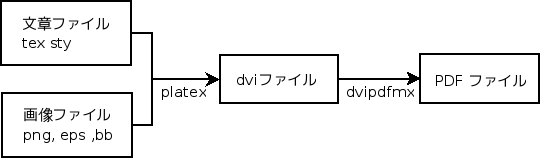
\includegraphics[width=120mm]{image200802/latex.png}
 \caption{\LaTeX で変換するイメージ}
 \label{fig:latex}
\end{center}
\end{figure}
\end{commandline}

\subsection{PDFへの変換}

変換の過程を簡単な図で示すと、図\ref{fig:latex}のようになります。

\begin{figure}[!htbp]
\begin{center}
 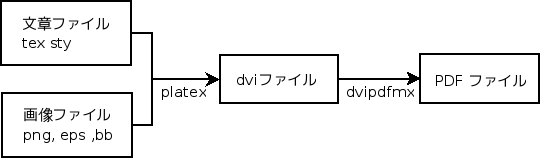
\includegraphics[width=120mm]{image200802/latex.png}
 \caption{\LaTeX で変換するイメージ}
 \label{fig:latex}
\end{center}
\end{figure}

コマンドで一つずつ変換をするならば、
\begin{commandline}
 $ platex debianmeetingresume200802-kansai.tex
 $ dvipdfmx debianmeetingresume200802-kansai.dvi
\end{commandline}

ですが、リポジトリから入手したものであれば、

\begin{commandline}
 $ make
\end{commandline}

\texttt{make}コマンドだけでファイルの更新があったファイルの変換などを
行なってくれます。

%%% 木下さん
\dancersection{バグレポートから参加するDebianパッケージ開発}{木下 達也}
\index{BTS}
\index{bugs.debian.org}
\index{bug tracking system}

\subsection{Debian開発への参加}
Debianは、どんな用途に使ってもよい、ソースを変更できる、
そのままでも変更版でもコピーして配布できる、
自由(フリー)なソフトウェアであり続ける、
ユーザーの、フリーソフトウェアコミュニティのための
オペレーティングシステムです。

Debian Projectは有志によって構成されています。
皆さんのできる範囲での参加・手助けを歓迎します。
まずはバグレポートから……

\begin{itemize}
 \item Debianプロジェクトホームページ \\
       \url{http://www.debian.org/}
 \item Debian社会契約 / Debianフリーソフトウェアガイドライン(DFSG)\\
       \url{http://www.debian.org/social_contract}
 \item How You Can Join\\
       \url{http://www.debian.org/devel/join/}
 \end{itemize}

\subsection{Debianパッケージを使っていて問題に遭遇!}
バグ?
設定誤り?
その他、環境依存の問題など?

さて、どうする?

\subsection{問題解決へ}

\begin{itemize}
 \item 現状は? 望ましい姿は? 再現できる?
 \item 問題の切り分け、仮説、実行、検証
 \begin{itemize}
  \item 設定をデフォルト値(または最小の設定)にしてみると?
  \item その他、条件を変えてみると?
 \end{itemize}
 \item ソースを見てみる?
\begin{commandline}
# apt-get update
(/etc/apt/sources.listにdeb-src行が必要)
$ apt-get source パッケージ名
\end{commandline}
\end{itemize}

\subsection{パッケージ情報の調べ方}

\begin{itemize}
 \item ファイルがどのパッケージに含まれているか検索
       \begin{itemize}
	\item インストール済のパッケージから検索
\begin{commandline}
$ dpkg -S /bin/ls
$ dpkg -S bin/apt
\end{commandline}
 \item Debian Packages ページで「パッケージの内容」を検索\\
 \url{http://packages.debian.org/}
 \item apt-file
\begin{commandline}
# apt-file update
$ apt-file -F search bin/ls
  (キーワードを末尾に持つパス)
$ apt-file search bin/apt
  (キーワードを含む名前のファイルを含むパッケージ)
\end{commandline}
\end{itemize}

\item Debian Bug Tracking System (BTS)\\
バグレポートを記録・追跡\\
\url{http://bugs.debian.org/}\\
\verb|http://bugs.debian.org/パッケージ名|\\
\verb|http://bugs.debian.org/src:ソースパッケージ名|
\end{itemize}

\subsection{メーリングリスト}
\begin{itemize}
\item Debian Mailing Lists\\
\url{http://lists.debian.org/}\\
(バグレポートやアップデート情報はメーリングリストにも流れています)

\item 日本語で相談するには、Debian JP Projectのメーリングリスト\\
\url{http://www.debian.or.jp/community/ml/}\\
\url{http://www.debian.or.jp/community/ml/openml.html}

\item 検索
 \begin{itemize}
 \item Google グループ: \url{http://groups.google.com/}
 \item Gmane Search: \url{http://search.gmane.org/} (日本語検索は難有り)
 \end{itemize}
\end{itemize}

\subsection{バグレポートの書き方}
\begin{itemize}
\item メールクライアントを起動

\item メール作成
 \begin{itemize}
 \item Text/Plainで
 \item 添付やgpg署名は可
 \end{itemize}

\item 宛先、題目を記入
\begin{commandline}
To: submit@bugs.debian.org
Subject: yaskkserv: funny dictionary order when skkdic-extra is installed
\end{commandline}

\item 本文の1行目からパッケージ名、バージョン、重要度を記入
\begin{commandline}
Package: yaskkserv
Version: 0.3.8-1
Severity: wishlist
\end{commandline}

\item Severity(重要度)
 \begin{itemize}
 \item critical (致命的)
 他のパッケージやシステムに影響する重大なバグ
 \item grave (重大)
 そのパッケージ自体の重大なバグ
 \item serious (深刻)
 ポリシー違反など、リリース品質でないと判断されるバグ
 \item important (重要)
 \item normal (通常)
 \item minor (軽度)
 \item wishlist (要望)
 \end{itemize}

\item 1行空けて、本文を記入、送信\\
(例: \url{http://bugs.debian.org/464812})
\begin{commandline}
Date: Sat, 09 Feb 2008 12:45:58 +0900 (JST)
From: Tatsuya Kinoshita <tats@vega.ocn.ne.jp>
To: submit@bugs.debian.org
Subject: yaskkserv: funny dictionary order when skkdic-extra is installed

Package: yaskkserv
Version: 0.3.8-1
Severity: wishlist
    
When the skkdic-extra package is installed, SKK-JISYO.JIS* in
skkdic-extra seem to be prefered over SKK-JISYO.L* in skkdic.
(e.g. when converting "あし", the default setting of yaskkserv
prefers "跫", "蹇", "蹙", ... over "足")

Please prefer SKK-JISYO.L* over SKK-JISYO.JIS* by default.

Thanks,
--
Tatsuya Kinoshita
\end{commandline}

\item Emacsユーザーなら`M-x debian-bug RET'
 \begin{itemize}
 \item 要debian-elパッケージ
 \item MewやWanderlustをデフォルトのEmacsメールクライアントに設定\\
 (/usr/share/doc/パッケージ名/README.Debianを参照)
 \end{itemize}
\end{itemize}

\subsection{Debian開発者との協同}
\begin{itemize}
\item Debian Package Tracking System (PTS)\\
ソースパッケージ毎のまとまった情報ページ\\
\url{http://packages.qa.debian.org/}ソースパッケージ名\\
(パッケージ名でもOK。ソースパッケージのページへ転送されます)

\item PTS subscribe, unsubscribe
 \begin{itemize}
 \item バグレポート、アップロード情報などを購読できる
 \item どの情報を購読するかは、メールでpts@qa.debian.orgへコマンドを送って変更\\
 \url{http://www.debian.org/doc/manuals/developers-reference/ch-resources.en.html}
 \end{itemize}

\item メールアドレス
 \begin{itemize}
 \item バグレポートへの返信: バグ番号@bugs.debian.org
 \item バグレポートの制御: control@bugs.debian.org
 \item パッケージメンテナ宛: パッケージ名@packages.debian.org
 \item Debian開発者宛、セキュリティ情報、非公開: security@debian.org
 \item Debianセキュリティチーム宛、非公開: team@security.debian.org
 \end{itemize}
\end{itemize}

%%% 倉敷さん
\dancersection{GPG 最初の一歩}{倉敷 悟}

GnuPG というと、「ああ、なんか apt-get の時にゴチャゴチャ文句言ってくる
アレか」といった印象をお持ちの方もおられるのではないかと思います。実は
Debian には様々な形で GPG が組みこまれていて、ssh 等にならぶマスト
アイテムといっても過言ではありません。このセッションでは、GPG の用途と
役割について簡単にご紹介した後、典型的な使用方法についてデモを行います。

\subsection{GPG の概要}
\index{gpg}
\index{gnupg}

端的に GPG とは何か、というと:
\begin{itemize}
 \item PGP 規格のフリーな実装 (特許の観点で、あるいは処理系として)
       \begin{itemize}
        \item 公開鍵暗号と共通鍵暗号のハイブリッド方式
       \end{itemize}
 \item メールやファイルの暗号化をするソフト
       \begin{itemize}
        \item 暗号化で盗聴を防ぐ (機密性/Confidentiality)
        \item 署名で改竄を防ぐ (完全性/Integrity)
        \item 信頼の輪で本人同定 (認証/Authentication)
       \end{itemize}
\end{itemize}

より詳しい解説は、下記 URL で読むことができます。

\begin{itemize}
 \item The GNU Privacy Guard \url{http://gnupg.org/} \\
       GnuPG 本家。ドキュメントは豊富ですが全部英語です。
 \item GNU Privacy Guard 講座 \url{http://hp.vector.co.jp/authors/VA019487/} \\
       日本語のポータル的なサイト。使い方を調べたい時に最適かと思います。       
 \item GnuPG (The GNU Privacy Guard) \url{http://www.math.s.chiba-u.ac.jp/~matsu/gpg/index.html} \\
       少し古い記事ですが、暗号機能の一般的な背景がわかりやすく解説されています。
\end{itemize}

\subsection{Debian における GPG}


\subsubsection{パッケージアーカイブ}

etch 以降、配布しているパッケージアーカイブの改竄防止のため、Release
ファイルに GPG でデジタル署名を施しています。APT でパッケージを取得する
際に、この署名を確認して、検証できない場合は警告が表示されるようになっています。

公式アーカイブの公開鍵はパッケージとして配布されているので、これをインス
トールしておけば、後は APT がよしなに面倒をみてくれます。

\begin{commandline}
kura@acacia:~$ dpkg -l | grep keyring
ii  debian-archive-keyring               2007.07.31                    GnuPG archive keys of the Debian archive
ii  debian-multimedia-keyring            2007.02.14                    GnuPG archive key of the debian-multimedia r
\end{commandline}

上記の例では debian-multimedia の鍵も入っていますが、公式でない
アーカイブでも、鍵が配布されていれば同じように検証をしてくれます。

\begin{itemize}
 \item SecureApt \url{http://wiki.debian.org/SecureApt}
\end{itemize}

\subsubsection{開発者の認証}

Debian では、GnuPG が本人の身分証明手段として広く浸透しており、特に
パッケージまわりで作業しようと思うと、なんだかんだで必要になります。

私に見えてる範囲では:
\begin{itemize}
 \item keysign に必要 (本末転倒ですが……)
 \item パッケージのビルドに必要 (必須ではない)
 \item mentors.debian.net への登録に必要
 \item Debian JP への参加に必要
 \item Debian {Maintainer|Developer} への応募に必要
\end{itemize}
といった場面で自分の GPG 鍵が必要です。また、ただ作るだけではなくて、
Debian Developer と keysign を行っておく必要もあります。

\subsection{名刺としての GPG 鍵}

現時点では、「Debian は使うだけだし、面倒だから別に要らないや」と
思うかも知れません。

ただ、他にもメリットがありますし、これを機会に是非 GnuPG を
使ってみてください。最初に必要なのは、たった一つ、「これから
作る鍵をちゃんと維持するぞ」という意気込みだけです。

\begin{itemize}
 \item デジタルな identity として
 \item こういったコミュニティでの名刺交換に
 \item 公開鍵基盤の身近な活用例として
 \item Debian Developer はレア
 \item keysign は結構おもしろい
\end{itemize}

\subsection{はじめてみよう}

\subsubsection{GPG 鍵を作る}
というわけで、自分の鍵を作ってみましょう。

\begin{commandline}
kura@acacia:~$ gpg --gen-key
gpg (GnuPG) 1.4.6; Copyright (C) 2006 Free Software Foundation, Inc.
This program comes with ABSOLUTELY NO WARRANTY.
This is free software, and you are welcome to redistribute it
under certain conditions. See the file COPYING for details.

gpg: directory `/home/kura/.gnupg' created
gpg: can't open `/gnupg/options.skel': そのようなファイルやディレクトリはありません
gpg: keyring `/home/kura/.gnupg/secring.gpg' created
gpg: keyring `/home/kura/.gnupg/pubring.gpg' created
Please select what kind of key you want:
   (1) DSA and Elgamal (default)
   (2) DSA (sign only)
   (5) RSA (sign only)
Your selection? 
\end{commandline}

まず、鍵の種類を聞かれます。ここはデフォルトのままで構いませんので、
何も入力せずに enter を押します。

\begin{commandline}
DSA keypair will have 1024 bits.
ELG-E keys may be between 1024 and 4096 bits long.
What keysize do you want? (2048) 
\end{commandline}

次に、鍵の流さを聞かれます。選択の目安としては、1024 は短かすぎるので NG、
デフォルトの 2048 はまぁ OK、計算機資源が余っているなら 4096 もアリ、
といったところでしょうか。

この例では、そのまま enter を押して、デフォルトの 2048 としています。

\begin{commandline}
Requested keysize is 2048 bits
Please specify how long the key should be valid.
         0 = key does not expire
      <n>  = key expires in n days
      <n>w = key expires in n weeks
      <n>m = key expires in n months
      <n>y = key expires in n years
Key is valid for? (0) 
Key does not expire at all
Is this correct? (y/N) y
\end{commandline}

次は、鍵の有効期限を選びます。私の場合、最初ここをどうするべきか困ったと
ころですが、これまで keysign してもらった方々のを見る限り、期限なしで問題
ないようです。

というわけで、そのまま enter を押して、確認にも y と答えます。

\begin{commandline}
You need a user ID to identify your key; the software constructs the user ID
from the Real Name, Comment and Email Address in this form:
    "Heinrich Heine (Der Dichter) <heinrichh@duesseldorf.de>"

Real name: KURASHIKI Satoru
Email address: lurdan@gmail.com
Comment: 
\end{commandline}

ここでは、自分の個人情報を設定します。keysign などでは、公的な証明書との
つきあわせを行いますので、その時に確認できる本名を入力する必要があります。
このあたり、日本のネットワーク文化とはいまひとつ馴染みがよくないかも知れ
ませんね。

GPG 鍵では、一つの ID に対して複数のメールアドレスを設定することができる
ので、Comment でそれを明示することができます。

\begin{commandline}
You selected this USER-ID:
    "KURASHIKI Satoru <lurdan@gmail.com>"

Change (N)ame, (C)omment, (E)mail or (O)kay/(Q)uit? O
\end{commandline}

最終的に、ユーザ ID がこうなりますよ、という確認です。問題ないので
O と入力します。

\begin{commandline}
You need a Passphrase to protect your secret key.

Enter passphrase:
Repeat passphrase: 
\end{commandline}

ここでパスフレーズを確認含めて 2 回入力します。パスフレーズには流さの
制限がないので、覚えやすい長さの英文を使うといいのではないでしょうか。

\begin{commandline}
We need to generate a lot of random bytes. It is a good idea to perform
some other action (type on the keyboard, move the mouse, utilize the
disks) during the prime generation; this gives the random number
generator a better chance to gain enough entropy.
.+++++++++++++++..++++++++++.++++++++++++++++++++++++++++++++++++++++.+++++++++++++++.+++++++++++++++.+++++.++
++++++++++++++++++.++++++++++>.++++++++++..............+++++

Not enough random bytes available.  Please do some other work to give
the OS a chance to collect more entropy! (Need 230 more bytes)
We need to generate a lot of random bytes. It is a good idea to perform
some other action (type on the keyboard, move the mouse, utilize the
disks) during the prime generation; this gives the random number
generator a better chance to gain enough entropy.
++++++++++......+++++..+++++.+++++.+++++.+++++..++++++++++.+++++.+++++++++++++++..+++++.++++++++++....+++++.++
+++++++++++++.++++++++++.++++++++++.+++++..+++++++++++++++..+++++>.++++++++++...>.+++++.......................
..............................................................................................................
...............+++++^^^^^
\end{commandline}

パスフレーズを入力した後は、乱数の生成のために、ブラウザでも開いて適当
に別の作業をします。そろそろいいかな、と元の画面に戻ると……

\begin{commandline}
gpg: /home/kura/.gnupg/trustdb.gpg: trustdb created
gpg: key 9751B54D marked as ultimately trusted
public and secret key created and signed.

gpg: checking the trustdb
gpg: 3 marginal(s) needed, 1 complete(s) needed, PGP trust model
gpg: depth: 0  valid:   1  signed:   0  trust: 0-, 0q, 0n, 0m, 0f, 1u
pub   1024D/9751B54D 2008-03-21
      Key fingerprint = 3AAA 2ED1 ACDA 49AE 4C68  66B9 CE7D E89C 9751 B54D
uid                  KURASHIKI Satoru <lurdan@gmail.com>
sub   2048g/B79D76D0 2008-03-21
\end{commandline}

このように完成しています。最後に表示された 「key fingerprint」のうち、
最後の 2 ブロックが自分の鍵の ID となります。

最後に表示されている部分で、「pub」の行が公開鍵、「sub」の行が秘密鍵を表
しています。

\begin{commandline}
kura@acacia:~$ ls -l .gnupg
合計 20
-rw------- 1 kura kura 1167 2008-03-21 16:06 pubring.gpg
-rw------- 1 kura kura 1167 2008-03-21 16:06 pubring.gpg~
-rw------- 1 kura kura  600 2008-03-21 16:06 random_seed
-rw------- 1 kura kura 1316 2008-03-21 16:06 secring.gpg
-rw------- 1 kura kura 1280 2008-03-21 16:06 trustdb.gpg
\end{commandline}

生成された鍵は、このように \$HOME/.gnupg/ に保管されています。これらの
ファイルは超大事なので、大切に取り扱うようにしましょう。

ちなみに、上の例で使っている鍵は、この記事のために作ったもので、もはや
存在しません。

\subsubsection{基本的な操作}

通常は、自分の鍵束 (\$HOME/.gnupg/*) には、

\begin{itemize}
 \item 自分の秘密鍵
 \item 自分の公開鍵
 \item 他の人の公開鍵
\end{itemize}

が入っています。これらの情報を確認する基本的なコマンドをご紹介します。
なお、鍵束の中で特定の鍵を指定するには、次のうちどれかが使えます。

\begin{itemize}
 \item 鍵 ID (ex. 0x9751B54D)
 \item 鍵 ID の 0x を省略 (ex. 9751B54D)
 \item 自分の UID の一部 (ex. KURA)
\end{itemize}
       
自分の鍵束にある公開鍵を一覧表示:
\begin{commandline}
$ gpg --list-keys
\end{commandline}

そのうち特定の公開鍵を表示:
\begin{commandline}
$ gpg --list-keys KURA
\end{commandline}

鍵指紋 (fingerprint) を確認:
\begin{commandline}
$ gpg --fingerprint KURA
\end{commandline}

鍵署名を確認:
\begin{commandline}
$ gpg --list-sigs KURA
\end{commandline}

\subsubsection{メールで使ってみる}

私が GPG を使うのは、主に gmail 上のメールアドレスなので、firefox のプラ
グイン「firegpg」を使っています。対象となる本文を選択して増えたボタンを
押すだけなので簡単に使うことができます。

\subsection{keysign の流れ}

\subsubsection{準備}

keysign のためには、次のものが必要です。

\begin{itemize}
 \item 公的な証明書 (鍵の持ち主の個人情報を証明できる、写真つきの書類)
       \begin{itemize}
        \item 運転免許
        \item 住民基本台帳カード
        \item パスポート
        \item 学生証
       \end{itemize}
 \item 署名してもらう鍵の指紋 (fingerprint) を印刷したもの
\end{itemize}

私の場合、鍵の指紋は手で書いたり、鍵表示をそのままコピー&ペーストして印刷したり
していました。

\begin{commandline}
pub   1024D/9751B54D 2008-03-21
      Key fingerprint = 3AAA 2ED1 ACDA 49AE 4C68  66B9 CE7D E89C 9751 B54D
uid                  KURASHIKI Satoru <lurdan@gmail.com>
sub   2048g/B79D76D0 2008-03-21
\end{commandline}

\subsubsection{当日}

公的な証明書を使って、keysign の相手とお互いに相手が相手であること
を確認し、用意した鍵指紋 (fingerprint) の印刷を交換します。

これだけです。簡単ですね。

\subsubsection{その後}

端末の前に戻ったら、まずは相手の公開鍵を手に入れましょう。

\begin{commandline}
$ gpg --keyserver subkeys.pgp.net --recv-keys 0x????????
\end{commandline}

keyserver は、相手が Debian Developer であれば keyring.debian.org も使え
ます。また、? の部分には、もらった鍵指紋 (fingerprint) の最後の 8 文字を入力します。

無事に公開鍵が入手できたら、それに署名をします。

\begin{commandline}
$ gpg --edit-key 0x????????
\end{commandline}

gpg のコマンドモードに入るので、
「uid (数字)」で署名をする uid を選び
(*マークがつきます)、
「sign」と入力します(fingerprint とメールアドレスを確認して署名)。

なお、相手が複数の uid を持っている場合、私は一通り全てに署名することに
しています。

終わったら、「quit」と入力し、変更を保存してください。

次のように署名の結果を表示して、自分の名前が表示されていることを確認してください。

\begin{commandline}
$ gpg --list-sigs 0x????????
\end{commandline}

ここまでで問題がなければ、相手の公開鍵をテキストファイルに export します。

\begin{commandline}
$ gpg --export -a  0x???????? > someones.key
\end{commandline}

後は、これを相手に送るだけです。添付するなり、本文に貼るなりして、メール
で送信します。相手の公開鍵で暗号化しておくとよいでしょう。

さて、相手も同じように署名をしてくれているはずですので、しばらくすると
メールで自分の公開鍵を送ってもらえるはずです。

届いたら、テキストファイルに export された鍵を自分の鍵束にとりこみ、
ついでなので公開鍵サーバにも送っておきます。
\begin{commandline}
$ gpg --import yours.key
$ gpg --keyserver subkeys.debian.org --send-keys 0x????????
\end{commandline}

? には、自分の公開鍵 ID を入力します。

\begin{itemize}
 \item 鍵署名 (Keysigning) \url{http://www.debian.org/events/keysigning}
\end{itemize}

%%% 大浦さん
\dancersection{Debian 開発者のコーナーの歩き方}{大浦 真}
\index{かいはつしゃ@開発者}
\index{www.debian.org/devel}

Debian プロジェクトの Web ページ内の
「Debian 開発者のコーナー」(\url{http://www.debian.org/devel/}) には、
Debian の開発や改良を行っていくために必要な情報が集まっています。
ただ、いろいろあり過ぎて、どこに何があるか分かりにくいです。
以下に有用なものをいくつか紹介します。

\subsection{基本}

プロジェクトに関する基本的な情報です。
\begin{itemize}
\item Debian の組織構成
\item Debian に参加する
\item 開発者データベース --- Debian 開発者の情報やプロジェクトのマシンを
  検索できます。
\item 投票情報 --- プロジェクトリーダの選挙結果などを参照できます。
\item さまざまなアーキテクチャ --- Debian は i386 以外にも多くのアーキテクチャに
  移植されています。
  Linux 以外への移植もあります。
\end{itemize}

\subsection{パッケージ開発}

パッケージを作成、メンテナンスするために必要な情報です。
メンテナが読むべき文書が集まっています。

\begin{itemize}
\item Debian ポリシーマニュアル --- Debian のシステムが守るべき技術的事項。
  いくつかサブポリシーもあります。
\item デベロッパーズリファレンス --- Debian のメンテナが守るべき手順と
  利用できるリソースの情報です。
\item 新規メンテナのためのガイド
\end{itemize}

\subsection{進行中の仕事}

パッケージのメンテナンスを進めていくために必要な情報です。

\begin{itemize}
\item バグ追跡システム
\item パッケージ追跡システム
\item Lintian レポート --- パッケージがポリシーを満たしているかどうか
  チェックすることができます。
\end{itemize}

\subsection{プロジェクト}

Debian 内のプロジェクトに関するリンクです。

\begin{itemize}
\item 品質保証 (Quality Assurance) グループ --- Debian 全体の品質を
  向上させるためのプロジェクト
\item 自動構築ネットワーク --- ソースパッケージを各アーキテクチャ用に
  自動的に構築します。
\item いろいろなカスタム Debian ディストリビューション
\end{itemize}

\subsection{その他}

その他の情報。

\begin{itemize}
\item Debian の ロゴとバナー
\end{itemize}

% 4月
%%% 名村さん
\dancersection{WindowsなPCでもDebianを楽しもう}{名村 知弘}
\index{Windows}
\index{coLinux}

\subsection{はじめに}
Windows上でしか動かないソフトがあったり、会社のPCがWindowsだったりと、
Windowsを完全に手放すことができない環境はまだまだ多いと思います。
そんなWindowsな環境にあっても、coLinuxがあればWindowsを起動しながらにし
て、お気軽にDebianを楽しむことができます。

coLinuxの設定から、Debianを楽しむまでの流れをご紹介します。

\subsubsection{coLinuxとは何か?}
coLinux(COoperative LINUX)とは、Windows上で動作するLinuxカーネルです。
coLinux上でDebianを動作させる場合、coLinuxパッチの当てられた専用のLinux
カーネル上でDebianが動作することになります。
DebianがWindows上の1つのアプリケーションとして動作するため、Windowsを使
いながら必要になった時にDebianを起動し使用することができます。

\subsubsection{なぜcoLinuxか?}
Windows上でDebianを使う環境としては、VMWareなどのPCエミュレータが考えら
れますが、PCエミュレータはオーバヘッドやメモリ使用量が大きく、全体的に動
作が重くなってしまします。
coLinuxはWindowsアプリケーションとしてLinuxが起動するため、PCエミュレー
タに比べ動作が軽いのが特徴となっています。
ただし、ディスプレイデバイスやサウンドデバイスが実装されていないため、単
体では音のでないCUI環境となります。
\footnote{別途VNCやXサーバ、サウンドサーバを使用することで、これら機能を使用することができます。}

\subsection{coLinuxインストール}
coLinuxでDebianを使用するには、
\begin{enumerate}
\item coLinuxのインストール
\item networkの設定
\item coLinuxの設定
\end{enumerate}
の3ステップを実行します。

以下では、Windows Vista\footnote{WindowsXPでも同様の手順で作業できると思
います。}での、TAP-Win32を使用したインストールのステップを簡単に説明しま
す。


\subsubsection{coLinuxのインストール}
coLinuxの配布サイト
\footnote{\url{http://sourceforge.net/projects/colinux/files}}から、
coLinuxのインストーラ\footnote{執筆時ではkernel2.6.22をベースとした
coLinux0.7.2が最新安定版となっています}をダウンロードします。

ダウンロードしたインストーラを起動し、デフォルトのままインストールを進め
ていくと、図\ref{fig:components}のような、インストールモジュールを選択す
る画面が表示されます。
ここではネットワークアダプタとして「TAP-Win32」を使用しますので、「SLiRP」
「WinPcap」のチェックを外してください。

\begin{figure}[htbp]
 \begin{center}
  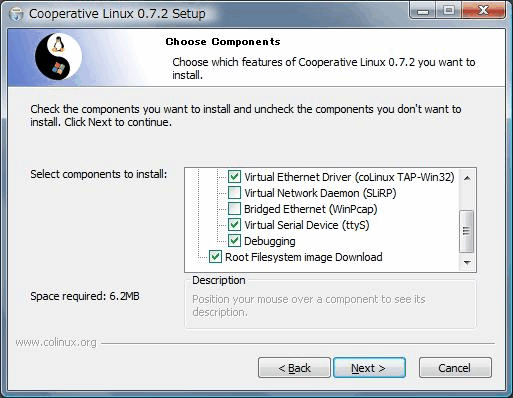
\includegraphics[width=100mm]{image200804/colinux_components.png}
 \end{center}
 \caption{インストールコンポーネントの選択}
 \label{fig:components}
\end{figure}

引き続きデフォルトのままインストールを進めていくと、図
\ref{fig:rootimage}のようなrootファイルシステムを選択する画面が表示され
るので、間違えずに「Debian」を選択してください。

\begin{figure}[htbp]
 \begin{center}
  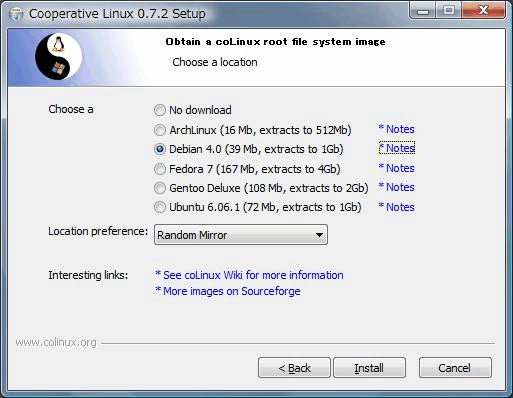
\includegraphics[width=100mm]{image200804/colinux_rootimage.png}
 \end{center}
 \caption{ルートファイルシステム選択}
 \label{fig:rootimage}
\end{figure}

あとは再びデフォルトのままインストールを進めると、インストール完了です。
ここで、「コントロールパネル」-「ネットワーク接続」を表示し、「ローカル
エリア接続 2」が作成されていると思いますので、右クリックし名前の変更を行
い、「TAP」に変更しておきます。

「ローカル エリア接続」 が2つ以上ある場合はプロパティを表示し、「接続の
方法」が「TAP-Win32 Adapter V8 (coLinux)」となっているものの名前を変更し
ます。

\subsubsection{network設定}
coLinuxの使用するネットワーク接続は、TAP-Win32(仮想ネットワークアダプタ)を使用します。
この仮想ネットワークアダプタは物理的にLANなどのネットワークに接続してい
ないため、ホストPCのReal NICを通じて物理的なネットワークに接続する必要が
あります。
物理的なネットワークに接続する方法として、ここでは以下の2つの方法をご紹介します。

Bridge接続を用いた方法

\begin{figure}[htbp]
 \begin{center}
  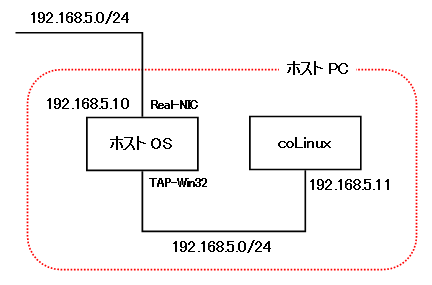
\includegraphics[width=100mm]{image200804/colinux_bridge.png}
 \end{center}
 \caption{Bridge接続を使用したネットワーク構成}
 \label{fig:bridge}
\end{figure}

Bridge接続では図\ref{fig:bridge}のように、TAP-Win32を通じてcoLinuxがReal
NICと同じサブネットに接続されるため、他のPCからもcoLinuxにアクセスするこ
とができます。
Real NICのネットワーク環境(固定IPやDHCPなど)に合わせて、coLinuxのネット
ワーク設定を行う必要があります。
長所としては、ネットワーク上の他のPCからcoLinuxに直接アクセスすることができます。
短所としては、ネットワークに接続されていない環境では、Windowsからも
coLinuxにアクセスすることができません。

設定は以下のようになります。
\begin{enumerate}
\item 「コントロールパネル」-「ネットワーク接続」を開きます。
\item 「ローカル エリア接続」と「TAP」を選択し、右クリックから「ブリッジ接続」を選択します。
\item 「ネットワークブリッジ」という接続設定が表示されたら完了です。
\end{enumerate}

ネットワーク接続の共有を用いた方法

\begin{figure}[htbp]
 \begin{center}
  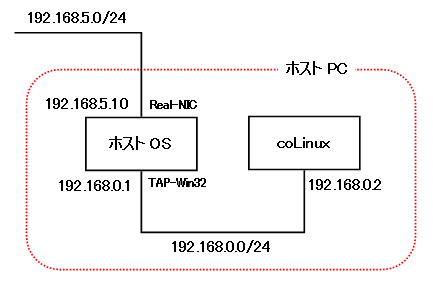
\includegraphics[width=100mm]{image200804/colinux_ics.png}
 \end{center}
 \caption{ネットワーク接続の共有を使用したネットワーク構成}
 \label{fig:ics}
\end{figure}

ネットワーク接続の共有では図\ref{fig:ics}のように、TAP-Win32はReal NICと
は異なるサブネットに参加し、ホストOSがNATになることで中継します。
TAP-Win32のIPアドレスは「192.168.0.1」固定となり、coLinuxは
「192.168.0.1/24」のIPを固定で割り当てることになります。
Real NICの接続しているサブネットが「192.168.0.0/24」の場合、IPアドレスが
バッティングしてしまうため、使用することができません。
長所としては、ネットワークに接続されていない環境でも、Windowsから常に
coLinuxに対して接続することができます。
短所としては、ネットワーク上の他のPCからはcoLinuxにアクセスすることができません。

設定は以下のようになります。
\begin{enumerate}
\item 「コントロールパネル」-「ネットワーク接続」を開きます。
\item 「ローカル エリア接続」を右クリックし、プロパティを表示します。
\item 「共有タブ」を開き、「ネットワークのほかのユーザーに、このコンピュー
      タのインターネット接続をとおしての接続を許可する」にチェックを入れ
      ます。
\item 「ホーム ネットワーク接続」は「TAP」を選択し、「OK」ボタンで閉じたら完了です。
\end{enumerate}

\begin{figure}[htbp]
 \begin{center}
  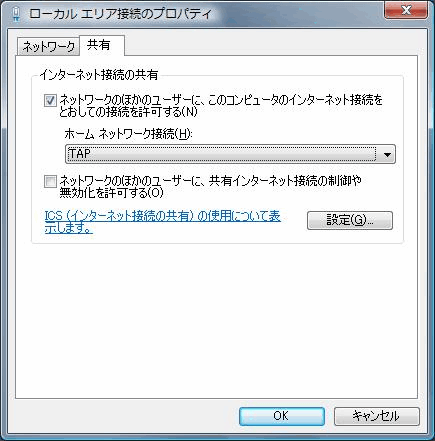
\includegraphics[width=100mm]{image200804/colinux_icssetting.png}
 \end{center}
 \caption{ネットワーク接続の共有の設定}
 \label{fig:icssetting}
\end{figure}

\subsection{coLinuxの設定}
coLinuxを起動するまでには、次の3つのステップが必要です。
\begin{itemize}
\item Debianのルートイメージの準備
\item swapディスクの準備
\item 設定ファイルの作成
\item coLinuxの起動
\end{itemize}

\subsubsection{Debianのルートイメージの準備}
coLinuxのインストール時にダウンロードされたDebianのルートイメージファイ
ルが、coLinuxインストールディレクトリに「Debian-4.0r0-etch.ext3.1gb.bz2」
というファイル名で作成されていますので、ファイルを展開\footnote{展開には、
bz2の展開ができるLhacaなどのツールが別途必要になります。}します。

展開すると「Debian-4.0r0-etch.ext3.1gb」というファイルが生成されるため、
分かりやすいように「fs-root-etch.img」などと名前を変更しておきます。

\subsubsection{swapディスクの準備}
coLinuxのインストールでは、swapファイルは用意されていないため、各自で用意する必要があります。
ここでは既に作成されたswapファイルをダウンロードできるサイトを利用してダウンロードします。

\url{http://gniarf.nerim.net/colinux/swap/}にアクセスし、「swap\_512Mb.bz2」をダウンロードします。

「swap\_512Mb.bz2」を展開すると、「swap\_512Mb」というファイルが生成され
るため、分かりやすいように「fs-swap-512.img」などと名前を変更しておきま
す。

\subsubsection{設定ファイルの作成}
これで必要なファイルは全てそろったので、coLinuxでDebianを起動するための設定を行います。

設定ファイルのフォーマットには、xmlを使用した方法と、独自のconfファイル
の2種類がありますが、ここではconfファイルを使用した方法を記載します。

coLinuxインストールディレクトリに「etch.conf」というファイルを作成し、以下の内容を記載します。

\begin{commandline}
kernel=vmlinux
initrd=initrd.gz
mem=512
#「c:\coLinux」は適宜coLinuxのインストールディレクトリで読み替えてください。
cobd0="c:\coLinux\fs-root-etch.img"
cobd1="c:\coLinux\fs-swap-512.img"
eth1=tuntap
root=/dev/cobd0
ro
\end{commandline}

coLinuxをインストールしたディレクトリに、「example.conf」というファイル
がありますので、必要であればこのファイルを参考に設定を変更してください。

\subsubsection{coLinuxの起動}
coLinuxには2通りの起動方法が用意されています。
\begin{itemize}
\item コンソールアプリケーションとして起動
\item サービスアプリケーションとして起動
\end{itemize}

以下にそれぞれの起動方法を記載します。

コンソールアプリケーションとして起動する方法\\
coLinuxのインストールディレクトリに、「colinux-daemon.exe」のショートカッ
トを作成し、プロパティから「リンク先」の末尾に「-t nt @etch.conf」を追加
します。

\begin{figure}[htbp]
 \begin{center}
  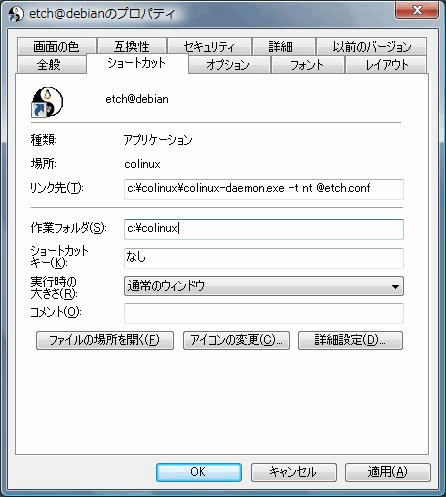
\includegraphics[width=100mm]{image200804/colinux_shortcut.png}
 \end{center}
 \caption{coLinux起動ショートカット}
 \label{fig:shortcut}
\end{figure}

このショートカットを起動すると、coLinuxがコンソールアプリケーションとして起動します。
コンソールアプリケーションとして起動しているため、コンソールを終了すると
当然coLinuxも終了してしまいます。

うっかり終了してしまうことを防ぐため、coLinuxをサービスアプリケーション
として起動する方法が用意されています。

サービスアプリケーションとして起動する方法\\
コマンドプロンプトを起動し、coLinuxのインストールディレクトリに移動し、
以下のコマンドを実行します。
「\verb|c:\coLinux|」は適宜coLinuxのインストールディレクトリで読み替えてください。
\begin{commandline}
colinux-daemon.exe "@c:\coLinux\etch.conf" --install-service
\end{commandline}

これでcoLinuxがサービスとして登録されました。ファイル名を指定して実行よ
り以下のコマンドを実行し、「Cooperative Linux」が登録されていることを確
認してください。
\begin{commandline}
%SystemRoot%\system32\services.msc
\end{commandline}

「スタートアップの種類」を「手動」に設定し、以下のコマンドでそれぞれ起動、
停止することができます。
\begin{commandline}
net start "Cooperative Linux"
net stop "Cooperative Linux"
\end{commandline}

%%% 大浦さん
\dancersection{Debian GNU/kFreeBSD}{大浦 真}
\index{kfreebsd}
\index{Debian GNU/kFreeBSD}

\subsection{Debian GNU/kFreeBSD とは}

Debian は、カーネルとして Linux だけをターゲットとしているのではない。
Debian GNU/kFreeBSD は、カーネルとして FreeBSD のカーネルを利用し、
その上に GNU C library と Debian のパッケージセットを移植したものである。
(カーネルだけを使っているので、``\textbf{k}FreeBSD'')

正式なリリースはまだだが、今回はそのインストール方法を紹介する。

\subsection{Debian GNU/kFreeBSD のインストール}

QEMU 上の仮想マシンにインストールする。

\begin{enumerate}
\item \url{http://glibc-bsd.alioth.debian.org/install-cd/}より
  インストール CD のダウンロード。
  現時点での最新版は、20080218 の日付のもの。
  \texttt{debian-20080218-kfreebsd-i386-install.iso}
  \begin{itemize}
  \item インストーラは、FreeBSD のインストーラを改造したものである。
    他のアーキテクチャで使われている Debian Installer は移植されていない。
  \end{itemize}
\item qemu 用のイメージの作成

  \$ \verb|qemu-img create -f qcow2 kfreebsd.img 10G|
\item qemu 起動

  \$ \verb|qemu -hda kfreebsd.img \| \\
  \verb|-cdrom debian-20080218-kfreebsd-i386-install.iso -m 512 -boot d|
\item FreeBSD のインストーラが起動したら Express を選択。
\item ハードディスクの設定。
  \begin{itemize}
  \item FDISK Partition Editor で slice の設定。
    Create Slice でハードディスク全体を選択。
  \item Boot Manager の設定。GRUB も使えるようだが、
    手動で設定する必要があるので、FreeBSD の Boot Magager を使う。
  \item FreeBSD Disklabel Editor。Partition の設定。
    ひとまず Swap Partition と / を作成。
  \end{itemize}
\item ベースシステムのインストール
  \begin{itemize}
  \item Choose Distribution で Minimal を選択。
  \item Choose Installation Media で CD/DVD を選択。
  \item CD から base system のインストールが始まる。
  \item Alt-F3 でコンソールに移る。
  \item tzdata の設定。
  \item popularity-contest の設定。
  \end{itemize}
\item インストールの終了と再起動。
  \begin{itemize}
  \item User Configuration Requested で No を選択。
  \item sysinstall Main menu に戻ったら Exit Install でインストーラを終了。
  \item 再起動。
  \end{itemize}
\item 再起動後の設定
  \begin{itemize}
  \item ユーザとしては、root のみが作成されている。
    パスワードなし。
  \item ネットワークの設定はなされていない。
    DHCP 環境の場合、dhclient を実行するとネットワークにつながる。
  \item ftp.debian-ports.org のアーカイブキーを取得。

    \$ \verb+wget -O - http://ftp.debian-ports.org/archive/archive_2008.key \+ \\
    \verb+| apt-key add -+
  \end{itemize}
\end{enumerate}

\subsection{問題点と今後}

\begin{itemize}
\item インストーラが行う設定が必要最低限のみ。
  一般ユーザの作成やネットワークの設定は自分で行う必要がある。
\item 基本的なパッケージでも移植できていないパッケージや
  きちんと動作しないパッケージが結構多い。
  (Debian GNU/Linux であることを前提して作られたパッケージが、
  GNU/kFreeBSD に持ってくるとビルドできないことがある。)
  \begin{itemize}
  \item console-tools、sysklogd、emacs22 など
  \item 現時点で、
    Architecuture: any のパッケージの 80\% ほどしかビルドできていない。

    \url{http://buildd.debian-ports.org/stats/}
  \end{itemize}
\item ハックのしがいあり。
  \begin{itemize}
  \item \url{http://glibc-bsd.alioth.debian.org/TODO}
  \item \url{http://glibc-bsd.alioth.debian.org/porting/PORTING}
  \end{itemize}
\end{itemize}

\subsection{関連リンク}

\begin{itemize}
\item \url{http://www.debian.org/ports/kfreebsd-gnu/}
\item \url{http://wiki.debian.org/Debian_GNU/kFreeBSD}
\item \url{http://glibc-bsd.alioth.debian.org/doc/} \\
  「Installing Debian GNU/kFreeBSD」
\item \url{http://tokyodebian.alioth.debian.org/html/debianmeetingresume200708se7.html} \\
  「Debian GNU/kFreeBSD のインストール」(第31回東京エリア Debian 勉強会資料)
\end{itemize}

%%% たかや
\dancersection{chrootからはじめる sid}{山下 尊也}
\index{sid}
\index{chroot}
\index{debootstrap}

sid って危険って言うけど、本当に危険なんですか?とか、unstableって名前が
怖かったりとか、はたまた、本日締切りの原稿とかあるのに、新しいバージョン
なものを触ってみたいとか、いろいろあると思います。

今回は、初めてsidの環境を触ろうと考えていらっしゃる方にお勧めなものを紹介します。

debootstrapを用いれば、chrootしたDebian環境を安易に構築する事が可能です。

今回は、/home/tommy/chroot/sid の下にchroot環境なsidを構築します。

\begin{commandline}
 $ sudo mkdir -p /home/tommy/chroot/sid
 $ sudo debootstrap sid /home/tommy/chroot/sid http://ftp.jp.debian.org/debian
I: Retrieving Release
I: Retrieving Packages
I: Validating Packages
I: Resolving dependencies of required packages...
I: Resolving dependencies of base packages...
・・・
I: Configuring klogd...
I: Configuring tasksel-data...
I: Configuring tasksel...
I: Base system installed successfully.
\end{commandline}

さっそく、作った環境にログインしてみましょう。

\begin{commandline}
 $ sudo chroot /home/tommy/chroot/sid /bin/bash
root@hoge:/# 
\end{commandline}

これでログイン出来ました。

基本的なパッケージしか入っていないため、/etc/apt/souces.list を更新し、
自分に必要なパッケージなどをいれましょう。

\begin{commandline}
root@hoge:/# vi /etc/apt/sources.list
\end{commandline}

/homeなどを共有したい場合は、以下のように親の/etc/fstabに書き加えます。

\begin{commandline}
 $ sudo vi /etc/fstab
/home           /home/tommy/chroot/sid/home        none    bind            0       0
/tmp            /home/tommy/chroot/sid/tmp         none    bind            0       0 
proc-chroot     /home/tommy/chroot/sid/proc        proc    defaults        0       0 
devpts-chroot   /home/tommy/chroot/sid/dev/pts     devpts  defaults        0       0 
\end{commandline}

ユーザ情報をコピーしましょう。

\begin{commandline}
 $ sudo cp /etc/passwd /home/tommy/chroot/sid/etc/
 $ sudo sed 's/\([^:]*\):[^:]*:/\1:*:/' /etc/shadow | sudo tee /home/tommy/chroot/sid/etc/shadow
 $ sudo cp /etc/group /home/tommy/chroot/sid/etc/
 $ sudo cp /etc/hosts /home/tommy/chroot/sid/etc/
\end{commandline}

chrootは、管理者権限がなければ使う事が出来ません。
dchrootは、chrootの環境のコマンドを一般ユーザの権限で実行する事を可能に
します。アプリケーションを用いたい場合などは、一般ユーザ権限で実行したい
場合が多いと思います。

\begin{commandline}
 $ echo ``mychroot /home/tommy/chroot/sid'' | sudo tee /etc/dchroot.conf
 $ dchroot -c mychroot (ログイン)
\end{commandline}

現在、experimentalな環境に iceweaselのバージョン3ベータがきています。
これを実行する事を考えてみましょう。
まず、experimentalな環境をインストール出来るように
/etc/apt/sources.listを編集します。

\begin{commandline}
 $ dchroot -c mychroot
 $ su -
root@hoge:/# vi /etc/apt/sources.list
deb http://cdn.debian.or.jp/debian/ sid main contrib non-free
deb http://cdn.debian.or.jp/debian/ experimental main contrib non-free
\end{commandline}

そして、experimentalなIceweaselをインストールします。

\begin{commandline}
root@hoge:/# aptitude install iceweasel/experimental
\end{commandline}

dchrootは、chroot環境以下に対して、一般ユーザの権限でコマンドを用いる事
も可能です。

\begin{commandline}
 $ dchroot -c mychroot -d iceweasel
\end{commandline}

これで、chroot環境内に構築しました experimental の Iceweasel を使う事が
出来ます。

chrootは現在動いているカーネル上に仮想OSを作成することから、
オーバーヘッドが比較的小さい事が大きな利点であると思います。

すでに安定版の Debian を使っているのであれば、chrootを用いれば、
簡単に不安定版の Debian のアプリケーションを利用する事が出きるので、
ちょっと触れてみたい方にはお勧めな方法の一つだと思うので是非試してみて下
さい。

\subsection{参考文献}

\begin{itemize}
\item \url{https://wiki.ubuntulinux.jp/UbuntuPackagingGuideJa/appendix-chroot} \\ The Ubuntu Packaging Guide 日本語版/chroot環境
\item Debian辞典 著者 武藤健志
\item \url{http://kmuto.jp/d/index.cgi/debian/debootstrap.htm} \\ KeN's
      GNU/Linux Diary Etch/Sidの上にSarge環境を作る方法
\end{itemize}


% 5月
\dancersection{ustream.tvを使った関西Debian勉強会中継の裏側}{野方 純}
\index{ustream.tv}

\subsection{はじめに}

4月29日の第12回関西Debian勉強会は、姫路での開催ということもあり、
ustream.tvのサービスを利用したインターネットビデオ中継を行いました。

ustream.tvはWindowsやMacの環境からは比較的簡単に利用できるようになってい
ますが、Debianでは少しつまづくところがあったので、その辺りを中心にTipsな
どを交えながら述べたいと思います。

\subsection{ustream.tvについて}

\subsubsection{ustream.tvとは}

ustream.tv(\url{http://www.ustream.tv/})とはWebブラウザとAdobe Flash
Playerを使いインターネットビデオ中継を行うことができるwebサービスです。
特徴としては、以下のようなものがあります。

\begin{itemize}
 \item WebブラウザとFlashプラグインとカメラがあればどこでもストリーミン
       グ中継ができる。
 \item ストリーミング中継は同時に録画でき、すぐにWeb上で公開できる。
 \item チャットがあるので視聴者も参加でき講演者は反応をダイレクトに知ることができる。
\end{itemize}

手軽にストリーミング中継ができることから、オープンソース系の勉強会では最
近よく使われるサービスです。

\subsubsection{ustream.tvを使って中継をするまでの流れ}

中継をするまでの流れを \url{http://www.ustream.tv/get-started} から引用
すると、このような感じになります。

\begin{enumerate}
 \item ustreamアカウントを作る(アカウントのある人はログインする)
 \item カメラをPCに接続する。
 \item ログインして"My Show"をクリック。
 \item "Name Your Show"にストリーミングの番組名を入力して"BROADCAST NOW"
       ボタンをクリック。
 \item Flashプラグインに「www.ustream.tvのカメラおよびマイクへのアクセス
       を許可しますか?」と尋ねられたら「許可」をする。
 \item "START BROADCAST"ボタンをクリックして放送開始。
\end{enumerate}

\subsubsection{中継をするために用意するもの}

ustream.tvの中継に必要なものをまとめました。必須なものについては、Debian
をデスクトップ環境にて利用されている方は普段使っているものばかりだと思い
ます。

\begin{itemize}
 \item 必須
       \begin{itemize}
	\item インターネット接続環境
	\item Debianがインストールされたマシン\verb|;)|
	\item Adobe Flashプラグイン
	\item Webブラウザ
	\item カメラ
	\item マイク
       \end{itemize}
 \item あれば便利
       \begin{itemize}
	\item オーディオミキサー
	\item IRCクライアント
       \end{itemize}
\end{itemize}

\subsection{実際に中継をする}

以上で中継に必要なものと手順がわかったので実際に中継してみました。

\subsubsection{中継ができた人とできない人がいた}

中継の実験をT氏と行っていましたが、筆者はほとんどトラブルもなく中継を行
うことができたのに対し、T氏は中継をすることができませんでした。
その理由を探っていくとどうやらFlash Playerに原因があることがわかりました。

\subsubsection{Flash Playerについて調べる}

\paragraph{Debian GNU/Linux(i386)で使えるFlash Playerについて}

Debianで使えるFlash Playerは3つ存在しますが、ustream.tvのサービスを利用す
るにはSWF V9が必要なので、フリーソフトウェアのGnashとSwfdecを使うことがで
きません。ですのでAdobe Flash Playerを使用することになります。

\begin{tabular}{llp{20em}}
 ソフト名(SWFバージョン) &ライセンス & インストール方法 \\ \hline
 Adobe Flash Player(SWF V9) & プロプライエタリ & non-freeセクション
         を追加してflashplugin-nonfreeをインストールするほかに、iceweasel2を使っ
         ていればユーザーディレクトリに自動インストールも可。 \\
 Gnash(SWF V7) & GPL V3 & aptitude install
         mozilla-plugin-gnashでインストール可 \\
 Swfdec(SWF V7) & GPL V2 & aptitude install
         swfdec-mozillaでインストール可
\end{tabular}

\paragraph{Adobe Flash Playerの制限}

Adobe Flash Playerは他のOSとほぼ同じバージョンなので、
同じように扱えるように見えますがLinux版には制限があります。

\begin{enumerate}
 \item 対応しているビデオAPIがVideo4Linux(V4L)のみ。(Kernel 2.6以降では
       V4L2が標準。V4Lは互換レイヤーで対応) \footnote{Adobe Flash Player
       10ではV4L2に対応予定。}
 \item サウンドの入出力にALSAを利用しているがサウンドデバイスを直接扱う。
 \item インプットメソッド(IM)の扱いがGTKのIM周りを考慮していない。
\end{enumerate}

1と2より使用するデバイスで中継ができた人とできない人に分かれました。3は直
接中継に関係ありませんが、Flashで作られたチャットクライアントを使う際に支
障が出ます。

\subsection{Adobe Flashで利用できるデバイスを考える}

使用できるデバイスに制限があるということが分かったので、Adobe Flashで使
えるデバイスについて考えてみます。

\subsubsection{カメラ}
\index{USB@USBカメラ}
\index{web camera}
\index{DV camera}
\index{v4l}
\index{video4linux}

PCに直接接続できるカメラは大きくわけて、このようなものがあります。

\begin{itemize}
 \item Webカメラ
       \begin{itemize}
	\item USB Video Class対応カメラ(linux-uvc)
	\item USB Video Class非対応カメラ(gspca, ov511, qc-usb)
       \end{itemize}
 \item DV(デジタルビデオ)カメラ
       \begin{itemize}
	\item IEEE1394接続
	\item USB接続
       \end{itemize}
\end{itemize}

USB接続のカメラでWebカメラと呼ばれるものは、USB Video Class(UVC)対応のものと
非対応なものでわけることができます。まずUSB Video Class対応カメラはドラ
イバのlinux-uvcがV4L2しか対応しておらずV4L互換レイヤーをサポートしていな
いのでV4Lしか使えないFlashでは使うことができません。
\footnote{The Flashcam Project
(\url{http://www.swift-tools.net/Flashcam/}) のflashcamを利用すればFlash
でもlinux-uvcカメラが使えるようです(未確認)}

USB Video Class対応カメラかそうでないかの見分け方は、

\begin{enumerate}
 \item 解像度が130万画素以上。
 \item Windowsドライバ不要とうたっている。
\end{enumerate}

どちらかに当てはまれば、UVC対応と見ればほぼ間違いないでしょう。


USB Video Class非対応のカメラについてはMicrosoft VX-1000とLogitech
Quickcam Expressの2種類使用しましたが、ドライバがV4Lに対応していたので楽
に使うことができました。ただUVC非対応のカメラはどのドライバに対応してい
るのか自分で見分けなければいけないことと、画素数が30万〜50万クラスのもの
しかないので画質に不満が出るかもしれません。


デジタルビデオ(DV)カメラについてですが、IEEE1394接続のカメラは転送される
データ形式がDV形式でV4Lは直接扱えないのでDV4Linuxを経由して使う必要があ
ります。映像についてはカメラとしての機能がしっかりしているので不満はない
と思います。


USB接続のDVカメラについては他のOSでは使用したとの記事を見かけたのですが、
まだ使用したことがないのでdebian上で使えるかどうかわかりません。


Linuxで使えるカメラについてまとめましたが、現時点では一長一短がありコレ
といっておすすめできるものがありません。なので、まだまだ試行錯誤は続くと
思われます。

\subsubsection{カメラの設定について}

使用したカメラの設定について述べます。

\begin{description}
 \item[Microsoft VX-1000/Logitech Quickcam Expressの設定] 

それぞれUVC非対応のカメラなので、VX-1000はgspca、Quickcam Expressは
qc-usbのカーネルモジュールを使います。標準のカーネルを使っている人は自分
の使っているカーネル用のカーネルモジュールが用意されるので、それをインス
トールしてください。

自分で作ったカーネルを使っている人はmodule-assitantを使ってカーネルモジュー
ルパッケージをインストールします。

\begin{commandline}
# aptitude install module-assistant
# m-a a-i gspca (VX-1000の場合)
# m-a a-i qc-usb (Quickcam Expressの場合)
\end{commandline}

あとはカメラを接続してブラウザでustream.tvに
アクセスするだけで使うことができました。

 \item[IEEE1394接続のDVカメラの設定]

IEEE1394接続のDVカメラは、DV4Linuxを経由して
ブラウザを起動する必要があります。

 \item[DV4Linuxのインストール]

DV4Linuxはdebianパッケージになっていないので配布元
(\url{http://dv4l.berlios.de/})からソースをダウンロードしてインストールす
る必要があります。

パッケージ作成練習と自分で使うために作った
sid用debianパッケージを作りましたが、きちんと
作っていないのでリスクを覚悟できる人だけ使ってください。

\url{http://regret.nofuture.tv/packages/dv4l_1.0-1_i386.deb}

\begin{commandline}
$ tar xvfz dv4l-1.0.tar.gz
$ cd dv4l-1.0/
$ ./configure
$ make
$ sudo make install
\end{commandline}

DV4Linuxをインストールするとvloopback
\footnote{仮想ビデオデバイスを作るカーネルモジュール。 
DV4Linuxとは別途インストールする必要があります。
Vloopback - Oss4art (\url{http://megaui.net/oss4art/wiki/Vloopback})}
を経由してDVカメラとデータをやりとりをするdv4lと、
直接DVカメラとやりとりするdv4lstartの2種類が
インストールされますが、dv4lは使うと画像が途切れ途切れに
送られてきて不安定なのでdv4lstartを使用します。

dv4lstartを使ってブラウザを起動するには、このようにします。

\begin{commandline}
$ dv4lstart iceweasel
\end{commandline}

統合デスクトップ環境を使っている方は
ショートカットアイコンを作っておくと便利です。

\end{description}

\subsubsection{参考}

\begin{itemize}
 \item DV4Linux \\
 (\url{http://dv4l.berlios.de/})
 \item ビデオキャプチャ:デバイス編 - Oss4art \\
            (\url{http://megaui.net/oss4art/wiki/%E3%83%93%E3%83%87%E3%82%AA%E3%82%AD%E3%83%A3%E3%83%97%E3%83%81%E3%83%A3:%E3%83%87%E3%83%90%E3%82%A4%E3%82%B9%E7%B7%A8>})
 \item Debian の最新 Linux kernel で DV 関係が全滅の件 - ほげめも \\
            (\url{http://www.keshi.org/blog/2007/08/debian_linux_kernel_disaster.html})
\end{itemize}

\subsection{サウンド}

基本的にはALSAで録音再生できるものであれば種類を問いませんが、Adobe
Flash はALSAの標準的なPCMデバイス名の default を使わず、最初に認識された
サウンドのハードウェアにつけられるデバイス名 hw:0,0 を利用して録音再生し
ようとします。最近のカメラはUSBサウンドを使ったマイクを内蔵している場合が
あり、音を拾わない場合はこの辺りをチェックするとよいでしょう。
\footnote{サウンドデバイスは cat /proc/asound/cards で確認することができ
ます。}

筆者の場合、USBサウンドユニットをALSAの設定ファイルの .asoundrc で
default に定義して使っていましたが、これではまったくFlashは録音再生をして
くれないので、サウンドカード認識の順番を変更することで対処しました。

\subsubsection{サウンドカードの認識順を変更する}

サウンドカードの認識順を変更方法は、/etc/modprobe.d/soundを変更する事に
よって行います。

サウンドカードの設定はこのような感じで指定するので

\begin{commandline}
alias snd-card-(番号) snd-(ドライバ名)
options snd-card-(番号) index=(番号)
\end{commandline}

実際にはこうなります。

\begin{commandline}
# alias snd-card-0 snd-hda-intel           元々の設定をコメントアウト
# options snd-hda-intel index=0 model=will 元々の設定をコメントアウト
alias snd-card-0 snd-usb-audio
options snd-usb-audio index=0
\end{commandline}

詳しい設定方法についてはカーネルソース付属のドキュメント、
Documentation/sound/alsa/ALSA-Configuration.txtを参照してください。

Flashのサウンド入出力について、contribセクションにある
flashplugin-nonfree-extrasoundパッケージを使えば、サウンドサーバーの
PulseAudioやEsound経由で変更できるようですが、筆者はデスクトップ環境に
KDEを使用しているので未確認です。

\subsubsection{参考}

\begin{itemize}
 \item Flash Player:Additional Interface Support for Linux - Adobe Labs \\
            (\url{http://labs.adobe.com/wiki/index.php/Flash_Player:Additional_Interface_Support_for_Linux})
 \item PulseAudio - Revolution Linux OpenSource projects \\
            (\url{http://pulseaudio.revolutionlinux.com/PulseAudio})
\end{itemize}

\subsection{本番で中継をするにあたってのTips}

ustream.tvで中継をするにあたり、障害になるデバイスの問題も解決できたので
基本的にはこれで中継を行うことができます。しかし、よりよい中継を行うため
に少しこだわってみます。

\subsubsection{マイクにこだわる}

ustream.tvでの中継を見ていると、マイクの音が小さすぎて会場で何を言ってい
るのかさっぱりわからない事があります。そうすると見ている方としては興ざめ
してしまうので、会場の音をきちんと拾うためにマイクにこだわってみましょう。

姫路からの中継では手持ちのサウンドミキサーとマイクを使用しましたが、サウ
ンドミキサーは6000〜8000円前後、マイクは一本3000円程度のものでも十分なので
用意しておくとよいでしょう。

BEHRINGERというメーカーのULTRAVOICE XM1800Sというマイクは3本セットで4000
円前後と非常にお買い得なのですが、マイクが複数本あると講演者と会場の音と
いうように分けて音を拾うことができるのでおすすめです。

\subsubsection{IRCクライアントでチャットに接続する}

ustream.tvはビデオストリーミングだけでなくIRCによるチャットも用意されてい
ます。しかし用意されているチャットクライアントはFlashで作られており日本語
がうまく扱えません。

ストレスをためながらチャットをするよりも、使い慣れたIRCクライアントを使っ
たほうがストレスもたまらず、ログなども取れたり便利なので、ustream.tvの
IRCサーバーに接続する設定を書いておきます。

\begin{center}
\begin{tabular}{|l|l|}
\hline
項目 & 設定内容 \\
\hline
サーバー名 & chat1.ustream.tv\\
ポート & 6667\\
文字コード & UTF-8\\
ユーザー名 & アカウントがある人はustreamアカウント名。なければ空にしておきます。\\
ニックネーム & 適当なニックネーム。\\
サーバーパスワード & ustreamアカウントのパスワード。アカウントのない人は必要ありません。\\
チャンネル名 & 中継アドレスのchannel以下に\#をつけたもの。\\
\hline
\end{tabular}
\end{center}

\begin{description}
\item[会場でチャットに参加している人も中継役]

ustreamのチャットは中継を見ながらチャットしているので当然ながら講演に対し
ての質問など意見が出てきます。ですが講演者が必ずしもチャットを見ている
わけではないので、会場でチャットに参加している人がいるなら、適当なころ合
いを見計らってチャットで出た質問などを視聴者に代わってしてあげてください。

そうすると会場はもちろん、インターネットを通じて見ている人も
盛り上がることは間違いないありません。

\end{description}

\subsubsection{画面を中継するには?}

今までカメラを使っての中継を書いてきましたが、実は/dev/videoに出力できる
ものなら、なんでも中継することができます。Screencast4Linuxを使えばPCの画
面をキャプチャして/dev/videoに流すことができるので、画面を中継することも
できます。

ちなみにScreencast4Linuxはまだdebianパッケージにはなっていません。
筆者はカーネルモジュールをパッケージにする方法をまだわかっていないので誰か挑戦してみて!

\subsubsection{参考}

\begin{itemize}
 \item Screencast4Linux: LinuxのX Window上で手軽にスクリーンキャスト \\
            (\url{http://yanbe.org/screencast4linux/})
\end{itemize}

\subsection{最後に}

本来ならばここまで大きくなることもなかったのですが、Adobe Flash Playerの
奇妙な仕様によりこんなに長くなってしまいました。

Adobeも「Open Screen Project」の一環として仕様やAPIの利用制限を撤廃したの
で、自由なソフトウェアのFlash Playerが発展し、早くこのようなバッドノウハ
ウに頼らなくなればと思っています。

\subsection{資料}

\subsubsection{ビデオデバイス周り}

\begin{itemize}
 \item V4LWiki \\
Video4LinuxのWiki。Linuxのビデオデバイス周りの情報は一通り揃っています。 \\
\url{http://linuxtv.org/v4lwiki/index.php/Main_Page}

 \item Welcome to QuickCam Team! - QuickCam Team \\
 Logitech Quickcam Teamのまとめサイト。ドライバの情報がまとまっています。\\
\url{http://www.quickcamteam.net/}

 \item VideoFourLinuxLoopbackDevice \\
仮想ビデオデバイスvloopbackのサイト\\
\url{http://www.lavrsen.dk/twiki/bin/view/Motion/VideoFourLinuxLoopbackDevice}

 \item AVLD - Another Video Loopback Device \\
もう一つの仮想ビデオデバイスの実装。\\
\url{http://allonlinux.free.fr/Projets/AVLD/}

 \item gstfakevideo \\
gstreamerに流すための仮想ビデオデバイス。gstreamerは鼻血が出るほどむずかしい。\\
\url{http://code.google.com/p/gstfakevideo/}

 \item Screencast4Linux: LinuxのX Window上で手軽にスクリーンキャスト \\
PCの画面をスクリーンキャストする。\\
\url{http://yanbe.org/screencast4linux/}

 \item DV4Linux \\
DVカメラとV4Lとやりとりするラッパーソフト。\\
\url{http://dv4l.berlios.de/}

 \item The Flashcam Project \\
UVCカメラとV4Lをやりとりするラッパーソフト。\\
\url{http://www.swift-tools.net/Flashcam/}
\end{itemize}

\subsubsection{その他}

\begin{itemize}
\item UstreamまとめWiki\\
ustream.tvで中継をするためのノウハウを集めたWiki。\\
\url{http://usy.jp/ustream/index.php?FrontPage}

\item ustream.tvからsmilevideoにアップロードするための講座 \\
ドワンゴの溝口氏によるustream.tvで録画したflvをffmpegを使ってエンコード
してニコニコ動画のsmilevideoにアップロードするまでの講座。\\
\url{http://www.ustream.tv/recorded/379002}

\item 表現のためのオープンソースソフトウェア Oss4art \\
EffecTV開発者のふくち氏によるLinuxマルチメディア系の情報を集めたWiki。\\
\url{http://megaui.net/oss4art/wiki/}

\item HowtoCast - dcastkit \\
八重樫氏製作によるDebian Liveベースのライブストリーミングに特化した
LiveCD dcastkitを使ったストリーミング方法。\\
\url{https://ssl.keshi.org/projects/dcastkit/trac.fcgi/wiki/HowtoCast}

\item Penguin.SWF\\
AdobeのLinux用Flash開発者のblog\\
\url{http://blogs.adobe.com/penguin.swf/}

\item Adobe Bug and Issue Management System\\
Flash Playerのバグトラック。まだできて間もないのであまりバグが登録されていません。\\
\url{https://bugs.adobe.com/flashplayer/}

\end{itemize}

\dancersection{Debian で始める Emacs エディタ}{木下 達也}
\index{emacs}
\index{GNU emacs}

\subsection{GNU Emacsとは}
GNU Emacsは、拡張・カスタマイズが可能なテキストエディタです。

GNUシステムの構成要素として1984年から開発が始まり、
現在もなお愛され続けています。

テキストエディタとしての基本的な機能に加えて、
複数の「バッファ」それぞれに応じた「モード」、
キー割り当てのカスタマイズ、Emacs Lispによるプログラミングが可能、
といった特徴があります。

その柔軟性は、文書作成、コーディングという用途に留まらず、
メール送受信、ウェブブラウズなどもこなせるほどです。

\subsection{Emacsのインストール}
\subsubsection{Debianパッケージ}

Debianではemacsパッケージをインストールすれば、Debian標準の
Emacsパッケージ(etchではemacs21、lennyではemacs22)がインストールされます。

\begin{commandline}
# apt-get install emacs
\end{commandline}

ウィンドウアプリケーションとして動かすのではなく、
端末でのみ利用したいのであれば、代わりに-noxパッケージ
(etchではemacs21-nox、lennyではemacs22-nox)を選べば、
依存関係が少なく、インストールサイズが小さくて済みます。

\subsubsection{Unicode日本語対応}

emacs21では、Unicode (UTF-8)日本語対応のためには、
別途mule-ucsパッケージが必要です。
(emacs22ではmule-ucs無しでも対応)

\begin{commandline}
# apt-get install mule-ucs
\end{commandline}

mule-ucsを有効にするには、設定ファイルのサンプル
\verb|/usr/share/doc/mule-ucs/examples/dot.emacs.ja|の内容を、
\verb|~/.emacs|の先頭の方に貼り付けておくとよいでしょう。
(emacs22でも有用な設定が含まれています)

注: mule-ucsを有効にする際には、やや時間がかかります。
また、\verb|~/.emacs|自身はUTF-8にしないように。
\verb|~/.emacs|読み込み前に環境変数でmule-ucsを有効にする方法もあります。
\verb|/usr/share/doc/mule-ucs/README.Debian|を参照。

\subsection{Emacsの利用法}

起動方法:

\begin{commandline}
emacs                 	通常起動
emacs -nw             	端末内で起動
emacs -q              	~/.emacsを読まずに起動
emacs -q -no-site-file	startupファイルを読まずに起動 (emacs22なら-Qでも可)
\end{commandline}

キーボード操作に慣れることで、Emacsをより快適に使えるようになります。

\begin{commandline}
C-x     Ctrlキーを押しながらx
M-x     ESCを押してからx  (またはAltキーを押しながらx)

ESC     EscキーまたはC-[
TAB     TabキーまたはC-i (字下げや補完に使う)
RET     EnterキーまたはC-m (改行と同時に字下げする場合にはC-j)
DEL     Back spaceキー
SPC     スペースキー

C-x C-c         Emacsを終了

C-p  上へ       C-n  下へ
C-b  左へ       C-f  右へ
C-a  行頭へ     C-e  行末へ

DEL     手前1文字を削除 (C-hはデフォルトではhelp-command)
C-d     1文字を削除
C-k     行末まで削除
C-o     行末までを次の行へ (改行を挿入、位置はそのまま)

C-x C-f         ファイルを読み込む
C-x C-s         ファイルを保存
C-x i           現在位置にファイルの内容を挿入
C-x C-w         別ファイルへ保存

C-x RET f       現在のバッファのcoding system(文字コード)を設定
C-x RET c       次に実行するコマンドのcoding systemを設定

C-v 次ページへ  M-v 前ページへ
M-< 先頭へ      M-> 末尾へ

C-s  前方検索   C-r  後方検索  (M-付きで正規表現)
M-%  置換  (C-付きで正規表現)

C-SPC マーク
C-w カット   M-w コピー   C-y ペースト

C-g     処理を中断
C-x u   Undo
C-l     現在行を中央にして再表示

C-x b バッファ移動   C-x k バッファ削除

C-x (   キーボードマクロ記録開始
C-x )   キーボードマクロ記録終了
C-x e   キーボードマクロ実行

C-x 2   ウィンドウ分割
C-x 1   他のウィンドウを削除
C-x 0   現在のウィンドウを削除

M-x     コマンド実行(Lisp関数を呼び出し)
M-:     ミニバッファで入力してLisp式を評価
C-x C-e 手前のLisp式を評価 (*scratch*ではC-jで評価・表示)
M-!     外部コマンド実行 (C-u付きで出力を現在位置へ挿入)

M-x help RET    ヘルプ
M-x info RET    マニュアル
M-x apropos RET 関数、変数等の名前を検索

\end{commandline}

カスタマイズ例:

\begin{commandline}
(global-set-key "\C-h" 'delete-backward-char)
(global-set-key "\C-ch" 'help-command)
(global-set-key "\C-z" 'scroll-down) ;; C-x C-z to use suspend/iconify
(global-set-key "\C-cg" 'goto-line)
(if (locate-library "iswitchb") (require 'iswitchb))
(if (fboundp 'iswitchb-default-keybindings) (iswitchb-default-keybindings))
(global-set-key "\C-cb" 'switch-to-buffer)
(setq visible-bell t)
(setq inhibit-startup-message t)
(if (fboundp 'menu-bar-mode) (menu-bar-mode -1))
(if (fboundp 'tool-bar-mode) (tool-bar-mode -1))
(if (fboundp 'auto-compression-mode) (auto-compression-mode 1))
\end{commandline}

\subsection{add-onパッケージ}

Emacs標準の機能だけでなく、さらに追加できるEmacs Lispパッケージがたくさんあります。

2008-05-13時点のDebian sidで、usr/share/emacsを含むパッケージ:

\begin{commandline}
# apt-file update
$ apt-file search usr/share/emacs | awk '{print $1}' | sort -u | cat -n
     1  a2ps:
     2  acl2-emacs:
     3  ada-mode:
     4  afnix:
     5  anthy-el:
     6  apel:
[...]
   256  yatex:
   257  yc-el:
   258  yorick-data:
   259  zenirc:
\end{commandline}

個人的なお勧め・注目パッケージ:

\begin{itemize}
 \item メールクライアント: mew, mew-beta, wl, wl-beta
 \item 引用ツール: mu-cite
 \item スケジュール管理: mhc, planner-el
 \item ウェブブラウザ: w3m-el, w3m-el-snapshot
 \item 日本語入力: ddskk, prime-el
 \item 辞書検索: lookup-el
 \item ローマ字での日本語検索: migemo
 \item 編集支援: muse-el, auctex, yatex
\end{itemize}

\subsection{emacsenパッケージ}

Debian sidに現時点で存在するemacsenパッケージ:

\begin{itemize}
 \item emacs22 (emacs22, emacs22-gtk, emacs22-nox)
 \item emacs21 (emacs21, emacs21-nox)
 \item xemacs21 (xemacs21-mule, xemacs21-mule-canna-wnn, xemacs21-gnome-mule,\\
       xemacs21-gnome-mule-canna-wnn, xemacs21-nomule, xemacs21-gnome-nomule)
\end{itemize}

非公式パッケージとして、Romain Francoiseさんによる
emacs-snapshotパッケージ(CVS版 Emacs 23.0.x)もあります。(\url{http://emacs.orebokech.com/})

Emacs Lisp add-onパッケージでは、emacsenそれぞれに応じた処理
(バイトコンパイル等)はインストール時に実施されるので、
パッケージはほぼ共通のものが使えます。


%% ここから月例

%===========================================================%
\begin{getsureiupdate}{月例 Debian GNU/kFreeBSD}{大浦 真}
\index{kFreeBSD}
  Debian Project の大浦です。(現在、京都在住)
  今月からこの場をお借りして Debian GNU/kFreeBSDの状況をお伝えすることに
  なりました。
  よろしくお願いします。

  Debian は、現在、その OS の中心として Linux カーネルを利用していますが、
  Debian GNU/kFreeBSD とは、カーネルとして FreeBSD のカーネルを利用し、
  その上に GNU C library と GNU のユーザランド、および、
  Debian のパッケージセットを移植したものです。
  FreeBSD のカーネルだけを使っているので、``\textbf{k}FreeBSD'' と
  呼んでいます。

  そんな Debian GNU/kFreeBSD は、開発途上にあり、
  Debian の一部として、まだ、正式にはリリースされていません。
  しかし、FreeBSD のインストーラを改造した kFreeBSD 用のインストーラも
  用意されていますし、
  kFreeBSD 用の buildd も設置されていますので、
  比較的簡単に実機やエミュレータ上で試すことができます。
  また、X.Org も使えますので、それなりに使うことができるようになっています。
  ただ、重要なパッケージで、buildd でビルドできず、
  バイナリが用意されていないものがあったり、
  用意されていてもまともに動作しないものがあったりもするので、
  まだまだ、いろいろとハックのしがいがあると思います。

  Debian GNU/kFreeBSD に関する情報は、以下の Debian Wiki のページに
  まとまっていますので、
  ぜひご覧下さい。

  \url{http://wiki.debian.org/Debian%20GNU/kFreeBSD}
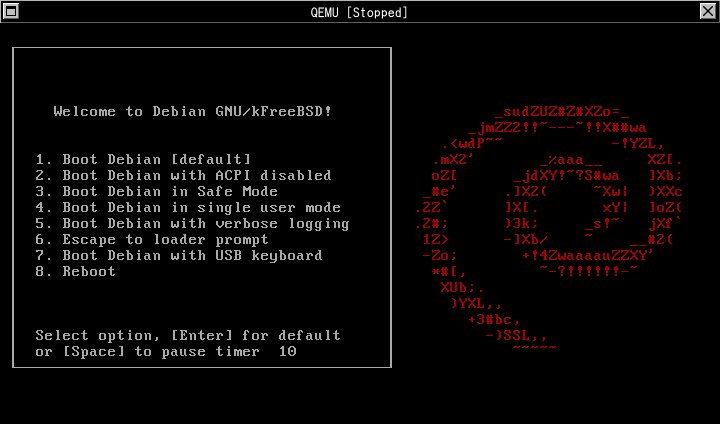
\includegraphics[width=1\hsize]{image200805/qemu-kfreebsd01.jpg}
\end{getsureiupdate}
%===========================================================%

%===========================================================%
\begin{getsureiupdate}{月例 Debian GNU/Linux SuperH port}{岩松 信洋}
\index{SuperH}
今月のDebian GNU/Linux SuperH 移植版の状況をお伝えします。

Debian/SH port は先月から加速しはじめました。
その理由として、フランス人の方が協力してくれることになったためです。
いまのところ、パッケージ用リポジトリを共同にしようということになっており、新しい
SH4用のリポジトリがフランスと日本にできました。

現在のステータスは、gcc-4.3 ベースでパッケージを作っています。
マシンが複数台あるのですが、builddをまだ1台しかセットアップしていません。
今月中には複数台セットアップしたいと考えています。

現在抱えている問題として、mesa のコンパイルに失敗するというものがありま
 す。
internal compiler error なので、調べるのは難しいですが、マクロ展開で
こけているところまで追いました。絶賛調査中です。

\begin{commandline}
gcc -c -I../../include -I../../src/mesa \
-I../../src/mesa/main \-I../../src/mesa/glapi \
-I../../src/mesa/math -I../../src/mesa/tnl 
-I../../src/mesa/shader \
-I../../src/mesa/shader/grammar \
-I../../src/mesa/shader/slang -I../../src/mesa/swrast \
-I../../src/mesa/swrast_setup -Wall -Wmissing-prototypes \
-O2 -g   -D_POSIX_SOURCE -D_POSIX_C_SOURCE=199309L \
-D_SVID_SOURCE -D_BSD_SOURCE -D_GNU_SOURCE -DPTHREADS\
 -DUSE_XSHM -DHAVE_POSIX_MEMALIGN  -I/usr/X11R6/include \
-std=c99 -ffast-math  -fno-strict-aliasing \
vbo/vbo_exec_api.c -o vbo/vbo_exec_api.o
vbo/vbo_exec_api.c: In function 'vbo_exec_fixup_vertex':
 vbo/vbo_exec_api.c:340: internal compiler error: Segmentation fault
 Please submit a full bug report,
with preprocessed source if appropriate.
See  for instructions.
 For Debian GNU/Linux specific bug reporting instructions,
 see .
\end{commandline}

今月のパッチ
\begin{itemize}
\item util-linux

sh4 アーキテクチャで mount パッケージが作成されない問題を修正。
\end{itemize}
\end{getsureiupdate}
%===========================================================%

%===========================================================%
\begin{getsureiupdate}{月例 Debian GNU/Hurd}{山本 浩之}
今月のDebian GNU/Hurdの状況をお伝えします。
\index{Hurd}
Debian GNU/Hurd は sid に入っていながら、未だ testing にすら入れてもら
 えず、冷や飯を食わされ続けていますが、それでもなお、 開発者たちは地味に
 頑張りつづけ、現在では K16CD インストールイメージをリリースするに至って
 おります。まずはこの K16CD-mini インストールイメージを VMware ディスク
 イメージにインストールしてみて問題点を調べてみました。

ユーザランドは基本的には Debian GNU/Linux と同じですが、いくつか Hurd
特有の呪文があります。

まず、ネットワークの設定ですが、/sbin/ifconfig にあたるものがなく、

\begin{commandline}
# settrans -fgap /servers/socket/2 /hurd/pfinet \
 -i eth0 -a 192.168.1.3 -g 192.168.1.1 -m 255.255.255.0
\end{commandline}

というように、settrans コマンドを使用します。また X を起動するには
かなり謎(?)な呪文を唱えないといけません:

\begin{commandline}
# console -d vga -d pc_mouse --repeat=mouse -d pc_kbd \
 --repeat=kbd -d generic_speaker -c /dev/vcs
\end{commandline}

現在のところ、Gnome や KDE のような統合デスクトップ環境は、build-dep なパッ
ケージが FTBFS バグのため揃っておらず、提供されていませんが、Window
Maker、Afterstep、IceWM、qvwm、ratposion、fvwm、ctwm などのウィンドウマネー
ジャが使用可能です。

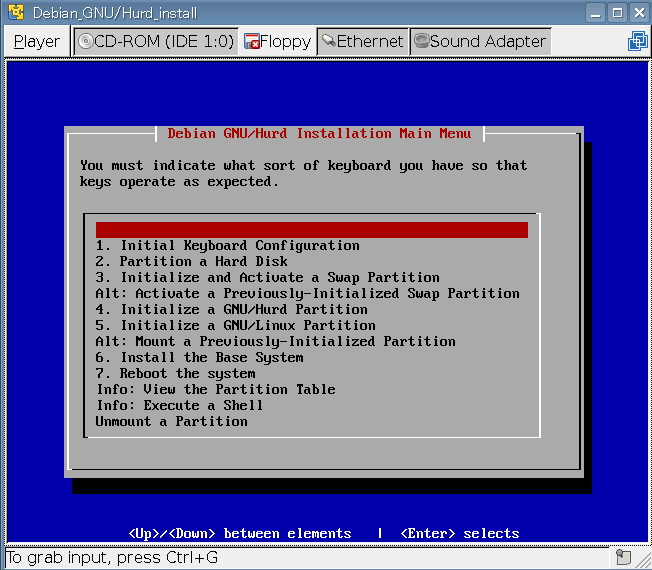
\includegraphics[width=1\hsize]{image200805/hurd0.png}
\end{getsureiupdate}
%===========================================================%

%===========================================================%
\begin{getsureiupdate}{月例 Nexenta Operating System}{上川 純一}
\index{Nexenta}
2008年4月号でインストールしてみた Nexenta Core Platform 1.0 で今月も何か
操作してみます。まず、ホストOSとのデータの交換の方法を確立してみます。

% まず、気が向いたので、kvm で起動してみます。グラフィック機能が超絶に遅い
% のと、ネットワークの接続ができなかった以外は高速に起動しているようです。
% kqemuで稼働させると数分かかるのに比べると高速です。

仮想マシン内部を快適に利用するために、まずSSH接続経由でのファイルシステムを共有をしてみ
 ましょう。
まず、ゲストOSの22番ポートをホストOSの2299番ポートとしてゲストOSを起動し
 てみました。
こうするとssh で localhostの2299番ポートにアクセスして
 ゲストOSにログインできます。

\begin{commandline}
dancer@host$ qemu -hda nexenta.cow -m 512 -redir tcp:2299::22 &
dancer@host$ ssh localhost -p 2299 
Password: 
Last login: Wed Apr 30 05:02:35 2008 from 10.0.2.2
dancer@vm1:~$ 
\end{commandline}

この状態でsshfs を利用するとゲストOSのパスをマウントして見ることができます。ホストOS
からゲストOSの/export/home/dancer にシームレスにアクセスすることができま
す。

\begin{commandline}
dancer@host$ sshfs localhost:  ./nexenta/  -p2299
Password: 
dancer@host$ ls -la nexenta/
合計 36
drwxr-xr-x 1 dancer uucp      9 2008-04-15 23:53 .
drwxr-xr-x 5 dancer dancer 4096 2008-04-30 14:05 ..
-rw------- 1 dancer uucp   1130 2008-04-23 13:05 .bash_history
-rw-r--r-- 1 dancer uucp    220 2008-03-19 18:07 .bash_logout
[以下略]
\end{commandline}

nexenta では各種ファイルを staffグループ (gid=10)が所有し、それがちょうど
Debian では uucpグループ (gid=10) が所有しているように見えています。
\begin{commandline}
dancer@vm1:~$ id dancer 
uid=1000(dancer) gid=10(staff) groups=10(staff)
\end{commandline}
\end{getsureiupdate}
%===========================================================%

\dancersection{Debian Trivia Quiz}{上川 純一}

ところで、みなさん Debian 関連の話題においついていますか?Debian関連の話
題はメーリングリストをよんでいると追跡できます。ただよんでいるだけではは
りあいがないので、理解度のテストをします。特に一人だけでは意味がわからな
いところもあるかも知れません。
漫然と読むだけではおもしろくないので、Debian 関連の話題から出題した以下の質問にこたえてみてください。
後で内容は解説します。
% FIXME: 転記すること
\begin{multicols}{2}

\subsection{問題}
出題範囲は\url{debian-devel-announce@lists.debian.org} に投稿された
内容からです。
 \santaku
 {Debian Developer になる前の人たちのための制度で最近 Open Beta を開始したのは何か}
 {Debian Maintainers}
 {Ubuntu}
 {Debian Account Manager}
 {A}

 \santaku
 {Debian Auditor は誰か}
 {Kalle Kivimaa}
 {Anthony Towns}
 {Sam Hocevar}
 {A}

 \santaku
 {Anibal Monsalve Salazar が参加したのはどのチームか}
 {Debian System Administrator}
 {Debian Cabal}
 {Debian Maintainer Keyring Team}
 {C}

 \santaku
 {debian/control に追加された Vcs-* フィールドでないのはどれか}
 {Vcs-git}
 {Vcs-rcs}
 {Vcs-Mtn}
 {B}

 \santaku
 {debian/control でパッケージのアップストリームプロジェクトのURLを記述す
 るためのフィールドは}
 {Homepage:}
 {URL:}
 {Upstream:}
 {A}

 \santaku
 {dpkg-buildpackage で並列ビルドをするためのコマンドラインオプションは}
 {-rfakeroot}
 {-j}
 {--nori1}
 {B}

 \santaku
 {2009年開催予定のDebconf9 の場所が発表された、その場所は}
 {Osaka}
 {Tokyo}
 {Extremadura}
 {C}

 \santaku
 {Policy 3.7.3.0 で追加されなかった変更は}
 {バージョン番号にチルドが利用できるようになった}
 {自由でないものはパッケージではない}
 {Debconf を利用する場合は国際化対応必須}
 {B}

 \santaku
 {gnuab にかわるリリースされていないDebian移植版のホスティングの場所はど
 こか}
 {\url{http://www.debian-doorstop.org/}}
 {\url{http://www.debian-ports.org/}}
 {\url{http://www.ubuntu.org/}}
 {B}

\subsection{問題}
\url{debian-devel-announce@lists.debian.org} に投稿された
内容からです。
 \santaku
 {Debian Miniconf 7が開催される、Linux Conf Au はいつ開始か}
 {1月28日}
 {1月29日}
 {1月19日}
 {A}

 \santaku
 {lintian は Debian パッケージのよくある間違いを検出してくれるツールであ
 る。 lintian.debian.org は全アーカイブに対して実行した lintian の実行結果を報告してくれているページだが、
 メンテナ単位のウェブページのURLが変更になった。どうかわったか?}
 {\url{http://www.youtube.com/email.html}}
 {\url{http://people.ubuntu.com/~liw/lintian/gutsy-i386-main/reports/maintainer/email.html}}
 {\url{http://lintian.debian.org/reports/maintainer/email.html}}
 {C}

 \santaku
 {dpkg のシンボルファイルで何が実現できるか?}
 {共有ライブラリなんてつかってられないので全部DLLにしてみた依存関係}
 {共有ライブラリはどんなバージョンでもよくなるような依存関係}
 {共有ライブラリのバージョン付きシンボルをベースにした依存関係}
 {C}

 \santaku
 {\url{http://wiki.debian.org/HelpDebian/Start} には何がかかれているか}
 {なぜDebianに貢献するべきか}
 {Debianはなぜ存在するのか}
 {GNUの存在意義}
 {A}

 \santaku
 {d-iでの翻訳作業の省力化のための工夫を Christian Perrierが実施した。
 それはメッセージを使われかたの優先度によって分割するものだったが、何分割にしたか}
 {5}
 {4}
 {3}
 {A}

 \santaku
 {Fonts task force (\url{http://wiki.debian.org/Fonts})は週次で何を確認するス
 クリプトを用意したか?}
 {Debianパッケージとしてはたしてどれだけのフォントファイルが存在するのか
 を棚卸する}
 {いかがわしい形のフォントを検出する}
 {うまく表示できないフォントを検出する}
 {A}

 \santaku
 {Lennyリリースに標準として含まれる予定のKDEはどれか}
 {KDE3.0}
 {KDE4.0}
 {KDE5.0}
 {A}

 \santaku
 {Debian-i18n meeting で {main,contrib,non-free}/i18n/Translation-* に対
 して何がおきたか}
 {Grisuが悟りを開いた}
 {AUTOBYHANDの仕組みを利用するようになった}
 {あきらめて変更しないことにした}
 {B}

 \santaku
 {FOSS.inの開催期間中にDDになったインド人は何人目のインド人DDか?}
 {1}
 {2}
 {4}
 {C}

 \santaku
 {insservでは何が実現できるか?}
 {自動でデータベースにinsert してくれる}
 {依存関係からinitスクリプトの実行順序を計算して実行}
 {ネームサービスの提供}
 {B}


\subsection{問題}
\url{debian-devel-announce@lists.debian.org} に投稿された内容からです。

 \santaku
 {lennyでのリリースゴールの1つにGCC 4.3でのビルドが通ることが挙げられているが、
 それに伴って変更する必要が最も多く生じるのは、どの言語で書かれたプログラムか?}
 {C}
 {C++}
 {Ruby}
 {B}
 
 \santaku
 {今のところlennyで完全に削除される予定なのは次のうちどれか?}
 {GNOME 1.x}
 {KDE 3.x}
 {Linux 2.x}
 {A}
 
 \santaku
 {Debianに宣伝力がないと感じたDebianプロジェクトリーダー (DPL) のSam Hocevarが提案したのは?}
 {イベント会場でDebianロゴの入ったシャツを着て練り歩くDebian Tank Top \& Brief Team}
 {ロゴやTシャツのデザインなどマーケティング面の任務を一手に引き受けるDebian Marketing Team}
 {Debianのマスコットキャラクター「でびにゃん」}
 {B}
 
 \santaku
 {3月頭の時点でlennyのリリースにとって致命的なバグ (RCバグ) は460ほどあるが、
 それを減らす方法として推奨されているのは?}
 {debian/changelogに「closes: \#xxxxxx」と書いて片っ端からパッケージをアップロードする}
 {バグ退治パーティー (BSP) を開いて片っ端からパッケージを非メンテナアップロード (NMU) する}
 {RCバグを放置しているパッケージメンテナを片っ端から呼び出して説教する}
 {B}
 
 \santaku
 {lennyはリリースされると何になる?}
 {Debian 4.1}
 {Debian 5.0}
 {Ubuntu 8.0}
 {B}
 
 \santaku
 {lists.debian.orgの新しい検索エンジンには何が用いられているか?}
 {Google Search}
 {Hyper Estraier}
 {Xapian Omega}
 {C}
 
 \santaku
 {新しいarmelアーキテクチャに関する現況として適切でないものは?}
 {lennyのリリースアーキテクチャに含まれている}
 {全パッケージの90\%がビルドされている}
 {パッケージをftp.debian.orgからダウンロードできるようになっている}
 {A}
 
 \santaku
 {次の開発者のうち、今年のDPL選挙に立候補したのは?}
 {Lucas Nussbaum}
 {Junichi Uekawa}
 {Steve McIntyre}
 {C}

\subsection{問題}
\url{debian-devel-announce@lists.debian.org} に投稿された内容からです。
 
 \santaku
 {パッケージの品質確認に有用な次のツールのうち、lennyおよびsidから削除されたものは?}
 {lintian}
 {linda}
 {piuparts}
 {B}
 
 \santaku
 {initスクリプトの実行順序を依存関係から自動的に決定できるようにすることがlennyのリリースゴールの一つになっているが、
 2008年4月16日現在、/etc/init.dにinitスクリプトを持つパッケージの数は?}
 {873}% パッケージの総数
 {857}% 対応済みパッケージの数
 {98}% 対応済みのパーセンテージ
 {A}
 
 \santaku
 {次のうち、Debian Installer Lenny Beta 1における改良点でないものは?}
 {NTPを用いた時刻合わせ}
 {volatileのサポートの追加}
 {Mac OS Xからのインストーラ起動のサポート}
 {C}
 
 \santaku
 {新たなDebianプロジェクトリーダー (DPL) に選ばれたSteve McIntyreが目標の一つに掲げているものは?}
 {Communications within the project}% 2008年DPLの標語の一つ
 {Make Debian sexy again}% 2007年DPLの標語の一つ
 {Welcoming people to the project}% 2006年DPLの2005年選挙での標語の一つ
 {A}
 
 \santaku
 {Debian Weekly Newsを復活させようというメールをdebian-devel-announceに流したのは?}
 {Martin Schulze}
 {Joey Hess}
 {Alexander Schmehl}
 {C}
 
 \santaku
 {lennyのリリースに関する現況として正しくないものは?}
 {GCC 4.3がデフォルトコンパイラとなり、それでコンパイルできないことがRCバグとなった}
 {lennyのリリースに向けて既に必須パッケージがフリーズされている}
 {デフォルトのsyslogデーモンをrsyslogに変更することが決定した}% まだ議論中
 {C}
 
 \santaku
 {dpkg 1.14.18で新たにいくつかのソースパッケージ形式がサポートされるようになったが、
 それらのうち次期デフォルトとされる「3.0 (quilt)」が持っていない機能は?}
 {ソースパッケージのupstream tarballとして複数のファイルを使用できる}
 {ソースパッケージのdiff.gzファイルを、適切に複数のパッチに分けてくれる}
 {ソースパッケージにDebian固有のバイナリファイルを挿入できる}
 {B}
 
 \santaku
 {今年のDPL選挙の投票率は?}
 {62.248\%{}}% 2000
 {53.084\%{}}% 2004
 {37.302\%{}}% 2008
 {C}
 
 \santaku
 {etchの次期ポイントリリースは「etch and a half」になるとされているが、
 そこに含まれる予定のLinuxカーネルのバージョンは?}
 {2.6.18}
 {2.6.24}
 {2.6.25}
 {B}
 
 \santaku
 {次の開発者のうち、新たにFTPマスターに任命されたのは?}
 {Sam Hocevar}
 {Joerg Jaspert}
 {James Troup}
 {B}
 
 \santaku
 {次の開発者のうち、Debian Marketing Teamのメンバーに任命されていないのは?}
 {Sam Hocevar}
 {Andreas Schuldei}
 {Moritz Muehlenhoff}
 {A}

 \santaku
 {Joerg Jaspert が DAM に任命されたのはSam Hocevar の任期の切れる何時間前か?}
 {24時間}
 {2時間}
 {-1時間}
 {B}

 \santaku
 {Software Design 2008年4月号155ページのgit-import-dscの事例にのっている
 パッケージ名は?}
 {ecasound}
 {pbuilder}
 {Windows Media Player}
 {A}

 \santaku
 {昨日 Debian 勉強会の参加メンバーで Debian Developer になったのはだれか?}
 {岩松}
 {小林}
 {Charles Plessy}
 {C}
 
 \subsection{問題}
 \url{debian-devel-announce@lists.debian.org}への投稿内容からです。
 
 \santaku
 {Joerg Jaspertがdakのソースコードに取り込んだ、Thomas Viehmannからのパッチとは?}
 {パッケージを受け取ったときにメンテナだけでなくスポンサーにもメールを送るようにするパッチ}
 {パッケージを受け取ったときに現在のカルマをメンテナに通知するパッチ}
 {パッケージを受け取ったときに現在のバグの一覧をメンテナに通知するパッチ}
 {A}
 
 \santaku
 {debhelperバージョン7では、何から学んだことを取り込んでいるか}
 {MSDN}
 {CDDB}
 {CDBS}
 {C}
 
 \santaku
 {新たにリリースマネージャになったのは?}
 {Andreas Barth}
 {Luk Claes}
 {Marc 'HE' Brockschmidt}
 {C}
 
 \santaku
 {Debianパッケージメンテナンスに関する自動通知メールにおいて、メールを生成したソフトウェアを示すのに使うよう提案されたメールヘッダは?}
 {X-Debian:}
 {X-Debian-Package:}
 {User-Agent:}
 {A}
 
 \subsection{問題}
 \url{http://www.debian.org/News/weekly/2008/01/}
 にある4月21日版です。
 
 \santaku
 {Siobh\'an O'MahonyとFabrizio Ferraroの研究ではDebianの統治システムの歴史を4つの時期に分けているが、そのうち1999年から2003年に当たるものは?}
 {Stabilizing Governance}% 2003-2006
 {Implementing Governance}% 1999-2003
 {Designing Governance}% 1997-1999
 {B}
 
 \santaku
 {Institute for Advanced Professional Studies Yankee groupの研究結果として適切でないものは?}
 {2006年と比べてDebianサーバのダウンタイムが41\%{}減った}
 {2006年と比べてネットワークに1台以上のDebianを入れているユーザが15\%{}から24\%{}に上昇した}
 {2006年と比べてDebianユーザが41\%{}減った}
 {C}
 
 \santaku
 {開発者のブログ記事を収集して表示するPlanet Debianに関して、Martin Joey Schulzeが始めたサービスとは?}
 {記事をメーリングリストとして購読できるようにするサービス}
 {すべての記事に対してコメントを一斉に送れるようにするサービス}
 {記事をSlashdotや各種ソーシャルブックマークサービスに容易に投稿できるようにするサービス}
 {A}
 
 \santaku
 {Christian Perrierによると、最近正式なDebian開発者として登録されたメンバーの女性率は?}
 {5\%{}}
 {10\%{}}
 {50\%{}}
 {B}
 
 \subsection{問題}
 \url{http://www.debian.org/News/weekly/2008/02/}
 にある5月9日版です。
 
 \santaku
 {WWWの生みの親として有名なTim Berners-LeeがWWW2008カンファレンスの基調演説でDebianについて述べたこととは?}
 {Debianのウェブページのように古臭いページは消えていく運命にある}
 {Debianのウェブページは様々な言語に地域化されており素晴らしい}
 {Debianのパッケージングシステムは素晴らしい}
 {C}
 
 \santaku
 {今年のGoogle Summer of CodeプログラムでDebian Projectのタスクを得た学生の人数は?}
 {6}
 {12}
 {24}
 {B}
 
 \santaku
 {5月9日現在、lennyのリリースに向けて進められている移行の状況として適切でないものは?}
 {Perlのバージョン5.10をlennyでデフォルトとするための移行作業が行われている}
 {既にlennyにおいてPythonのデフォルトがバージョン2.5になっている}
 {Rubyのバージョン1.9をlennyでデフォルトとするための移行作業が行われている}
 {C}
 
 \santaku
 {4月18日に何人のDebian正式開発者が追加されたか?}
 {9}
 {19}
 {29}
 {B}
 
\end{multicols}

\dancersection{Debian Trivia Quiz 問題回答}{上川 純一}

\begin{multicols}{2}
 Debian Trivia Quiz の問題回答です。
 あなたは何問わかりましたか?
 \\
 %回答はdebianmeetingresume2008-natsu.jqzというファイルに生成されるので、
 %それを手動でコピペして使う。
 % ここからコピペ
 % FIXME 問題が全部はいったらコピペすること
 %(progn (next-line 1)(insert-file "debianmeetingresume2008-natsu.jqz") )
1. A\\
2. A\\
3. C\\
4. B\\
5. A\\
6. B\\
7. C\\
8. B\\
9. B\\
10. A\\
11. C\\
12. C\\
13. A\\
14. A\\
15. A\\
16. A\\
17. B\\
18. C\\
19. B\\
20. B\\
21. A\\
22. B\\
23. B\\
24. B\\
25. C\\
26. A\\
27. C\\
28. B\\
29. A\\
30. C\\
31. A\\
32. C\\
33. C\\
34. B\\
35. C\\
36. B\\
37. B\\
38. A\\
39. B\\
40. A\\
41. C\\
42. A\\
43. C\\
44. C\\
45. A\\
46. B\\
47. C\\
48. A\\
49. B\\
50. C\\
51. B\\
52. C\\
53. B\\

\end{multicols}



\printindex

\cleartooddpage

{
\large
\begin{itembox}{\bf 『あんどきゅめんてっど でびあん』について}
本書は、東京および関西周辺で毎月行なわれている『東京エリア Debian 勉強会』および
『関西エリア Debian 勉強会』で
使用された資料・小ネタ・必殺技などを一冊にまとめたものです。
収録範囲は東京エリアは勉強会第35回から第40回、関西エリアは
第10回から第13回まで。
% FIXME: 回数を修正すること。
内容は無保証、つっこみなどがあれば勉強会にて。
\end{itembox}
}

\vspace*{15cm}
{\color{dancerlightblue}\rule{\hsize}{1mm}}
\vspace{2mm}

\includegraphics[width=2cm]{image200502/openlogo-nd.eps}
\noindent \Large \bf あんどきゅめんてっど でびあん 2008年夏号\\ \\
% FIXME 開催日がわかったら更新すること
\noindent \normalfont 2008年8月16日 \hspace{5mm}  初版第1刷発行\\
\noindent \normalfont 東京エリア Debian 勉強会/関西エリア Debian 勉強会 (編集・印刷・発行)\\
{\color{dancerdarkblue}\rule{\hsize}{1mm}}

\end{document}
